\documentclass[lang=cn,newtx,scheme=chinese]{elegantbook}

% ------------------------------------------------
% 基本编码与字体设置
% ------------------------------------------------
\usepackage{ctex}
\usepackage{anyfontsize}
\usepackage{amsmath}
\renewcommand{\normalsize}{\fontsize{12pt}{15pt}\selectfont}  % 字体大小和间距设置
\setlength{\parskip}{0.5em}  % 段落间距设置
\usepackage{fancyvrb}
\fvset{fontsize=\small} % 代码字体大小设置

% ------------------------------------------------
% 表格与绘图宏包
% ------------------------------------------------
\usepackage{tabularx}
\usepackage{booktabs}
\usepackage{array}
\usepackage{tikz}
\usetikzlibrary{arrows.meta}
\usepackage{subcaption}
\usepackage{babel}

% ------------------------------------------------
% 颜色与代码展示
% ------------------------------------------------
\usepackage{xcolor}
\usepackage{listings}
\newcommand{\ccr}[1]{\makecell{{\color{#1}\rule{1cm}{1cm}}}}
\definecolor{customcolor}{RGB}{135, 206, 235}
\colorlet{coverlinecolor}{customcolor}

% ------------------------------------------------
% 超链接设置
% ------------------------------------------------
\usepackage{hyperref}
\hypersetup{
	colorlinks=true,
	linkcolor=black,
	citecolor=black,
	urlcolor=black
}

% ------------------------------------------------
% 文档信息设置
% ------------------------------------------------
\title{社会科学研究方法}
\subtitle{因果推断}
\author{元景阳}
\date{2025年8月}
\version{1.0}
\setcounter{tocdepth}{3}
\logo{logo.jpg}
\cover{cover.png}

% ------------------------------------------------
% 正文部分
% ------------------------------------------------
\begin{document}

\maketitle
\frontmatter
\tableofcontents

\mainmatter
\chapter*{前言}
\addcontentsline{toc}{chapter}{前言}

当亚里士多德在《物理学》中提出``四因说''时,他或许未曾预见两千三百年后社会科学面临的根本性挑战——如何在复杂的社会系统中构建兼具解释力与预测力的因果模型。从古典政治哲学对城邦政体的类型学归纳,到霍布斯《利维坦》中对社会契约论的个人主义方法论演绎,再到当代计量经济学``可信性革命''的技术突破,人类对社会现象的理解始终在``理论建构''与``经验验证''的张力中螺旋上升。本书正是对这一认识论传统的当代回应,旨在构建连接政治哲学思辨传统与数据科学实证范式的桥梁。

本书旨在为社会科学研究者提供一套完整的方法论体系,具体内容安排如下:

\begin{itemize}
    {\fangsong \item 第一章从哲学基础切入,探讨客观现实主义与主观建构主义的认识论分野,回顾科学革命以来自然科学方法向社会科学的延伸历程,并介绍实用主义、逻辑实证主义、结构主义和后实证主义等重要方法论流派。
    
    \item 第二章聚焦研究选题的确立,指出如何避免``garbage in, garbage out''的陷阱,提出好问题的五项标准,并系统阐释理论建构、变量操作化与研究设计的核心环节。
    
    \item 第三章为定量分析奠定数学基础,涵盖微积分、线性代数、概率论与统计推断等必备知识,帮助读者建立坚实的工具储备。
    
    \item 第四章梳理因果推断的理论源流,从计量经济学的发展历程谈起,深入介绍潜在结果框架、``可信性革命''的核心思想,以及结构式因果模型、do算子与反事实推理等现代方法。
    
    \item 第五章探讨统计推断在多元回归分析中的应用,包括OLS估计、异方差处理与模型选择等核心内容。
    
    \item 第六章进入因果推断的实践应用,从经典实验设计到观测数据分析,从简单因果路径到复杂因果网络,系统覆盖RCT、断点回归(RD)、工具变量(IV)、双重差分(DID)等常用方法,并结合实际案例,帮助读者在不同研究情境中选择恰当的因果推断策略。}
\end{itemize}

计算机技术的迅猛发展为复杂社会现象的建模和分析提供了前所未有的便捷工具。从传统回归分析到深度学习算法,从抽样调查到通过网络爬虫获取的海量数据,计算社会科学正在重塑我们理解和解释社会现象的方式。本书将介绍如何利用现代统计软件和编程工具进行数据处理,使读者能够紧跟当代社会科学研究的技术前沿。通过将经典方法论与现代计算工具相结合,本书致力于帮助读者在掌握扎实理论基础的同时,具备运用现代研究方法解决实际问题的能力。

全书试图构建起连接政治哲学思辨传统与数据科学实证范式的桥梁,相信无论是初学者还是有一定基础的研究者,都能从本书中获得有益的启发和实用的指导。

\begin{flushright}
元景阳 \\
2025年8月
\end{flushright}

\newpage
\chapter{研究方法的哲学基础}
\section{存在论}
世界如一枚硬币,既有可测量的金属材质,又有雕刻其上的图案花纹。想要真正理解世界,在掂量硬币的重量的同时,也要欣赏其花纹与光影。想象此刻的你站在桂林山水前。“美”是山水的客观属性,还是你内心的主观感受?这个简单的问题揭示了人类认识世界的两种基本方式------客观与主观。\textsuperscript{\cite{1}}

\subsection{客观---现实主义}

客观---现实主义范式认为,社会现实是客观存在,独立于个人的意识和认知的。根据这一范式,社会现象有其独立的客观特征,可以通过科学方法进行观察、测量和分析。以此为基础或出发点,客观---现实主义在认识论上和方法论上,强调经验主义或实证主义,认为知识来源于对现实世界的经验观察和数据收集,并追求识别社会现象之间存在可识别的因果关系。这样的存在论可以称为客观主义、唯物主义、现实主义等,为了避免语境转换造成的词不达意,我们复合使用客观---现实主义。

\subsection{主观---建构主义}

主观---建构主义范式认为,社会现实是通过人类的主观认知和社会互动建构而成的。根据这一范式,社会现象的意义和现实是由个体和群体共同赋予和解释的,强调研究者理解人们如何通过互动和交流来建构人们所处的社会世界。就有了“社会世界是建构的而不是独立于人主观意识的客观存在”这一论断或认识。例如,身份是一种通过个体主观体验及社会互动形成的社会现象,涉及家庭、朋友等多元关系中的意义协商,并受文化差异(如性别、种族定义)、社会权力结构(如阶级地位)及规范标签(如刻板印象)的动态影响,具有流动性和历史情境性。

不同的存在论流派的争论由来已久,在科学革命后的当今世界,客观---现实主义无疑占据着中心与主导的地位,因此后文的主干部分介绍的也基本都是客观---现实主义一派。

\section{科学革命的开端}

\subsection{方法论自然主义}

肇始于文艺复兴时期的方法论自然主义是影响科学发展的最早的哲学流派,这一时期科学研究与经院哲学的诠释在方法论上分家,伽利略开启了以方法论自然主义弥合二者分歧的思路,即科学研究的方法论不涉及到宗教思考------超自然存在及终极真理仍然由教会掌握。人们认识世界的方式自此发生了重大转变,在渐进积累了一整个中世纪之后,那颗著名的苹果,砸落到一个聪明的脑瓜的那刻,其意义远大于物理课本上的万有引力定律,这一事件象征着这样一个时代来临:\textbf{从仰望神谕转向俯察人间,从依赖经典权威转向依靠观察、实验与理性推理}。

\subsection{自然科学向社会科学的延申}

亚里士多德在其哲学体系中提出了著名的“四因说”,系统阐述了自然界事物生成与变化的原因。他认为,真正理解一件事物,必须同时揭示其四种不同类型的因:其一为质料因(causa materialis),即构成事物的物质基础;其二为形式因(causa formalis),即事物所具有的结构、形状或本质特征;其三为动力因(causa efficiens),即促使事物生成、变化或运动的外在力量;其四为目的因(causa finalis),即事物存在或运动的目的与功能,是亚里士多德因果论中最具目的论色彩的一环。通过这一因果分类法,亚里士多德力图超越机械式的因果解释,建立一个涵盖本质、结构、动力与目的的多维解释体系,成为西方形而上学和科学方法论的重要源流。

作为比较政治学研究先驱的亚里士多德开创性地对一百多个希腊历史上存在过的城邦政体进行了详细的分类,然而遗憾的是,亚氏首先构建了三个母本(君主、贵族与共和),而现实中存在的城邦政体只是母本的衍生。与其师柏拉图不同的是,亚里士多德并不试图以\textbf{纯粹的理念哲人王}统领人世,而是客观上承认了多元利益造就的多元共治和多元共赢。

中世纪的宗教为与王室和解(竞争)而逐步放弃了原始的蒙昧精神,科学的幼苗在柏拉图和亚里士多德两位的精神遗风的培育下逐步发芽,终于长成一棵果树,硕果挂满枝头。所以,当那颗苹果落下时,选择研究它为何落下、如何落下,开启了一场重塑人类理解自身与世界方式的伟大征程。

追随亚里士多德的脚步,中世纪的学者往往从目的论的角度出发,追问\textbf{苹果为何落下}------是否符合上帝的旨意或某种终极目的。而科学革命后的思想家们则更关注“\textbf{苹果是如何掉下来的}”,即试图通过观察和实验揭示支配自然现象的普遍规律。这种从“为什么”向“如何”的转变,标志着认识论的重大转向。

认清普遍、可量化的规律后的人们决定对自我生活的世界进行反思,从各个方面汇集而来的思考很快构建起经验主义的基本框架。有趣的是,尽管经验主义的思想渊源可以追溯到中世纪晚期的经院哲学家如\textbf{奥卡姆的威廉},但作为一种系统的哲学传统,它在17至18世纪的英国得到了系统发展,并由此得名“\textbf{英国经验主义}”。与此同时,欧洲大陆上则兴起了以笛卡尔为代表的\textbf{理性主义}传统,强调通过先验推理获得知识。这两种认识论路径之间的张力贯穿了近代西方哲学的发展历程,也深刻影响了后来社会科学的方法论基础。

\subsection{唯理主义与经验主义}

随着自然科学的哲学转向,社会科学也开始寻求自身的认识论基础。其中,政治学作为一门独立学科的形成过程尤为典型。被誉为“君主宝鉴”的《君主论》始终是我们讨论政治学转型绕不开的书籍,在羞于谈论权谋却总以权谋私的政治环境中,一本较为直白的书最是难得。尽管如此,真正开启政治科学进程的更多还是霍布斯所著的《利维坦》一书。

此处转引包刚升老师对本书的评述:\textsuperscript{\cite{2}}

\begin{quote}
	{\fangsong 霍布斯认为,人类因无限欲望陷入持续冲突。为摆脱混乱,需建立拥有绝对权力的国家。他强调人性中的自我保全本能和对权力的追求,认为\textbf{资源竞争、相互猜疑和荣誉感}导致自然状态下的生活\textbf{危险、贫困且短暂}。为此,霍布斯提出“社会契约”:人们为安全自愿转让权利,形成国家(即“利维坦”),以维持秩序、抵御外敌。国家可通过征服或契约建立。尽管国家可能存在问题,但其存在是避免无政府混乱的必要条件。
		
	霍布斯在《利维坦》中结合个人主义与科学逻辑分析政治问题,为现代政治理论奠定基础。他的思想影响深远,即使后来如洛克等思想家也难以忽视其贡献。总体而言,霍布斯标志着西方近现代政治理论的重要转折,其关于\textbf{人性、权力与国家关系}的思考至今仍有影响力。}
\end{quote}

也就是从在这里开始,经验主义内部出现了分歧。不难看出,尽管霍布斯演绎出的\textbf{人性恶}的观点不无道理,但以\textbf{社会契约}来予以改善则不完全是一种现实的观察,更多是脑海中的推演。哈耶克在《自由秩序原理》(又译《自由宪章》)一书中也有过精彩的论述:\textsuperscript{\cite{3}}

\begin{quote}
	{\fangsong 唯理主义(理性主义)传统假定,人生来就具有智识的和道德的秉赋,这使人能够根据审慎思考而形构文明;而进化论者(经验主义者)则明确指出,文明乃是经由不断试错、日益积累而艰难获致的结果,或者说它是经验的总和,其中的一部分为代代相传下来的明确知识,但更大的一部分则是体现在那些被证明为较优越的制度和工具中的经验\ldots\ldots{}}
\end{quote}

洛克接过霍布斯的“社会契约”概念,却对其进行了合乎资本主义发展现实的革命性的改造。在洛克看来,自然状态并非全然“污秽、残酷与短暂”,而是存在着“自然法”的约束,人拥有\textbf{生命、自由、财产}等不可剥夺的“自然权利”。政府的建立,并非为了创造秩序本身,而是为了更好地\textbf{保护}这些先在的权利。当政府违背契约、侵犯权利时,人民有权\textbf{反抗}。洛克的学说,为自由主义奠定了基石:\textbf{个人权利优先、有限政府}和\textbf{基于同意的统治}。

在\textbf{认识论}层面,洛克在其著作《人类理解论》中提出了“白板说”,认为人的心灵如同一块空白的石板,所有知识皆来源于感官经验。这种观点体现了典型的英国经验主义传统。与之形成鲜明对比的是法国哲学家笛卡尔,他在《第一哲学沉思集》中提出“我思故我在”,强调理性思维先于经验,主张通过演绎推理获取知识。这两种路径不仅构成了近代哲学的基本张力,也深刻影响了社会科学中的研究范式之争,经验主义和唯理主义之间经久不息的较量正式开启。

\section{社会思潮的产生与认识论的发展}

社会思潮的形成是复杂而多维的过程,它不仅反映了特定历史时期的社会矛盾与人们的思想追求,也深刻影响了科学研究的方法论选择与发展路径。从文艺复兴到启蒙运动,从现代自然科学迈向现代社会科学,不同的哲学思想和社会理论相互交织、碰撞,共同塑造了我们今天所看到的知识版图。在主要的社会思潮之中,最具有影响力的分别是自由主义、保守主义和社会主义。

\subsection{自由主义的双重面向}

古典自由主义(如洛克、亚当·斯密)深受英国经验主义熏陶。它强调\textbf{个体的感官经验、自由探索和利益驱动}是理解社会的基础。自由市场被视为一个庞大的、自发的“发现程序”,通过无数个体的互动(试错),信息得以传播,资源得以有效配置。这种对社会秩序形成的理解,更倾向于进化理性,即秩序是无数个体行动无意中形成的复杂结果,而非某个单一头脑的设计。

然而,自由主义内部也存在强烈的\textbf{理性主义}倾向,尤其在涉及政治制度设计时(卢梭的社会契约论、孟德斯鸠的三权分立以及美国的联邦党人的政治实践),各种说辞无不使人相信人类理性能够设计出保障自由、限制权力的制度框架。边沁的功利主义更是将理性计算推向极致,试图用“最大幸福原则”作为衡量政策和社会制度的科学标尺。

约翰·密尔在《逻辑体系》一书中给出了归纳的因果五法,参考互联网哲学百科全书对此做出的论述如下:\textsuperscript{\cite{4}}

密尔对归纳法的著名论述揭示了信念的经验基础。他提出了五种用于识别因果关系的实验探究方法,旨在从现象前后的情境中找出那些通过\textbf{不变法则}与现象相关联的因素。简言之,我们通过在多种情境下观察现象,来判断某种因果关系是否成立,以下五种方法为此提供了系统性依据:

\vspace{0.8em} % 手动调整间距	
\begin{itemize}
	\item
	\textbf{求同法}
	:若多个不同情境中某一现象都出现,且唯一共同因素存在,则该因素可能是原因。
	\item
	\textbf{求异法}
	:若某现象在一个情境中出现,在另一个中不出现,而两者仅有一个因素不同,则该差异因素可能是原因。
	\item
	\textbf{求同求异联合法}
	:结合前两种方法:一方面找现象出现时的共同因素,另一方面看该因素缺失时现象是否也消失,从而更可靠地确定因果关系。
	\item
	\textbf{共变法}
	:若某因素变化时,现象以固定方式随之变化,则二者存在因果联系。
	\item
	\textbf{剩余法}
	:从复杂现象中剔除已知原因引起的变化,剩余部分可归因于尚未解释的因素。
\end{itemize}

\subsection{保守的怀疑主义?现代因果关系起源}

如果说自由主义(尤其是其古典形式)更多地根植于经验主义对个体行动和自发秩序的观察,那么保守主义的核心则是对\textbf{抽象理性设计社会蓝图}的深刻怀疑,其思想源泉同样与经验主义传统,特别是对\textbf{历史实践、传统智慧与制度演化}的重视紧密相连。埃德蒙·伯克在《法国革命论》中的论述,堪称保守主义对理性主义社会工程学的经典批判。

伯克并非反对变革本身,而是反对基于抽象理念(如“天赋人权”、“社会契约”)的激进革命。他认为社会是一个\textbf{复杂的有机体},是历经漫长岁月、由无数代人的实践、妥协和智慧沉淀而成的。其\textbf{制度、习俗和传统}(即使存在不完美)包含了超越个体理性的“集体智慧”,是维系社会秩序和情感纽带的基石。盲目地用“理性”的手术刀切割这些传统,试图按照某种乌托邦蓝图重建社会,其结果必然是灾难性的------法国大革命后期的恐怖似乎印证了他的预言。

\textbf{休谟与康德:重塑因果关系之基}

与此同时,在\textbf{认识论}层面,英国哲学家大卫·休谟对自由主义中的唯理主义一面的打击是毁灭的。休谟以其\textbf{彻底的怀疑主义}动摇了经验主义乃至所有声称具有必然性的知识的根基。他的核心洞见直指科学方法和理性社会设计的核心------何为因果,参考互联网哲学百科全书对此的论述如下:\textsuperscript{\cite{5}}

休谟对因果关系的客观性提出了根本性质疑。他将人类知识分为两类:\textbf{观念间的关系}(如数学、逻辑,具有普遍必然性)与\textbf{事实的知识}(如自然科学,依赖于经验观察)。科学知识属于后者,其核心是因果推理。

根据休谟的观点,因果关系由三个基本观念构成:\textbf{时间先后、空间邻近和必然联系}。
	
\begin{itemize}
    \item
    \textbf{时间先后}:原因必须先于结果。若B在A之前发生,说A导致B是不合逻辑的。
    \item
    \textbf{空间邻近}:因果事件需在空间上接近。例如,英国人扔石头的同时中国窗户破碎,并不意味着两者有因果关系。
    \item
    \textbf{必然联系}:仅有时序与邻近不足以构成因果。例如,喷嚏与灯灭同时发生并不等于因果关系。休谟指出,我们从未在经验中直接观察到“A导致B”这一“必然联系”。我们观察到的只是事件A(如太阳升起)之后恒常地伴随着事件B(如石头变热)。这种恒常联结经过反复观察,形成了我们心理上的“习惯性联想”。因此,当我们看到A发生时,便预期B会发生。这种预期并非基于理性的逻辑必然性,而是一种心理习惯。人们常犯的一个低级错误便是,由于既往的感知如此,便武断地认为因果关系当然存在,然而这种论证始终没有开端,即为\textbf{循环论证}。
\end{itemize}

休谟的论证极具颠覆性。他以“黑天鹅”问题和“火鸡理论”为例,说明基于归纳法的因果规律永远存在被证伪的可能性。这揭示了科学知识的或然性(probabilistic)而非必然性。休谟的结论是:因果关系并非世界固有的客观属性,而是人类主观心理的产物。这一观点动摇了科学知识的根基,引发了“休谟问题”,即如何为基于经验归纳的科学知识寻求普遍必然性的辩护。因此,尽管休谟以其怀疑主义闻名,他对因果本质的质疑,反而促使后来的科学家和哲学家更加谨慎地对待变量之间的关联,从而推动了\textbf{实验设计与统计因果推断}的发展。

休谟的怀疑论“将康德从独断论的迷梦中唤醒”。康德承认休谟的正确之处——我们无法从经验中直接感知因果必然性。但他拒绝接受科学知识因此丧失客观性的结论。康德的解决方案是提出“\textbf{哥白尼式的革命}”:不是我们的认识去符合对象,而是对象必须符合我们的认识形式。\textsuperscript{\cite{6}}

康德认为,人类的心灵并非一块被动接受经验的“白板”,而是拥有先天的认知结构。他将认知分为三个层次:\textbf{感性}(提供时空直观形式)、\textbf{知性}(运用范畴进行综合判断)与\textbf{理性}(追求系统性统一)。其中,“\textbf{因果性范畴}”是知性十二范畴之一。

康德主张,因果关系是我们认识世界所必需的先验框架。我们之所以能将杂乱的感官印象组织成有序的经验,正是因为心灵主动运用了因果性范畴。例如,我们看到杯子掉落并破碎,不是先观察到事件序列再归纳出因果,而是\textbf{在观察的瞬间,就已通过因果范畴将这两个事件理解为“因”与“果”}。因此,因果关系虽然不是“物自体”的属性,但却是“现象界”的普遍必然法则。

康德通过“\textbf{先天综合判断}”为科学知识奠基。像“一切发生之事皆有其原因”这样的判断,既非分析判断(不依赖经验),又非后天综合判断(具有普遍必然性),而是基于先验范畴的先天综合判断。科学知识的客观性,源于所有人类共享相同的认知结构,即“\textbf{主体间性}”。

\textbf{刘易斯与玻尔:潜藏在休谟悖论第三点中的反事实条件句}

20世纪哲学家大卫·刘易斯试图超越本体论争论,为因果关系提供一个可操作的逻辑定义。他认为,因果关系的本质是“\textbf{反事实依赖}”。\textsuperscript{\cite{7}}

其核心模型是:\textbf{事件A是事件B的原因,当且仅当,若A没有发生,则B就不会发生}。这可以形式化为一个反事实条件句:“If A ×, then B would ×.”

刘易斯借助“\textbf{可能世界}”理论来阐释这一概念。为了评估一个反事实语句的真假,我们需要考察一个与现实世界尽可能相似的“最邻近可能世界”。在该世界中,A不发生,然后观察B是否发生。如果在那个最邻近的世界中B也没有发生,则反事实依赖成立,A是B的原因。

例如,验证“堵车导致迟到”:设想一个与现实世界几乎完全相同,唯一区别是交通畅通的世界。如果在这个世界里你准时到达,则说明堵车是迟到的原因。

然而,该理论面临“\textbf{抢跑问题}”的挑战:苏西和鲍比同时向窗户扔石头,苏西的石头先击中并导致窗户破碎,鲍比的石头随后才到。虽然窗户破碎反事实依赖于苏西的石头击中(若未击中则不破),但并不反事实依赖于苏西扔石头(因为即使苏西没扔,鲍比的石头也会打破窗户)。为解决此问题,刘易斯引入“\textbf{因果链条}”概念,认为即使首尾事件无直接反事实依赖,但若存在一个由反事实依赖环节构成的链条(苏西扔石头 $\rightarrow$ 石头飞行 $\rightarrow$ 窗户破碎),则因果关系依然成立。

21世纪,计算机科学家朱迪·珀尔将因果推理推向了数学化与算法化的新阶段。他批评刘易斯的理论虽有洞见,但缺乏可操作性,因其依赖于难以衡量的“可能世界相似性”。\textsuperscript{\cite{8}}

珀尔提出了“干预模型”,其核心思想是:$X$是$Y$的原因,当且仅当,对$X$进行人为干预会改变$Y$的概率分布。这用数学语言表达为: $P(Y | do(X)) \neq P(Y)$。

这里的关键是区分“观察”与“干预”:

\begin{itemize}
    \item \textbf{观察}:$P(Y | X)$ 表示在观察到$X$发生的条件下,$Y$发生的概率。这只能揭示相关性。
    \item \textbf{干预}:$P(Y | do(X))$ 表示我们主动将$X$设定为某个值(无论其自然原因是什么),然后观察$Y$的概率。这才能揭示因果性。
\end{itemize}

珀尔的模型旨在解决“混杂因子”问题。例如,观察发现吸烟者肺癌发病率更高,但这可能是因为存在一个共同原因$Z$(如压力或基因),它既导致人吸烟,也导致人患癌。仅靠观察无法区分是$X \rightarrow Y$,还是$Z \rightarrow X$且$Z \rightarrow Y$。而通过随机对照实验(RCT)——随机分配人群吸烟或不吸烟(即$do(X)$)——可以打破$X$与$Z$的自然关联,从而隔离出$X$对$Y$的纯粹因果效应。

在此基础上,珀尔发展了结构因果模型(Structural Causal Models, SCM)和因果图(Causal Diagrams),用有向图明确表示变量间的因果机制。这使得因果推理可以被编码为计算机算法,使人工智能从“相关性机器”升级为能进行“因果推理”的智能体。珀尔认为,反事实推理能力(如“如果我当初那样做,结果会怎样?”)是自由意志的基础,而他的模型正是将这种能力形式化的尝试。

\subsection{社会主义的实证与实践}

激进自由主义者的左转在社会思潮中形成了社会主义,而在认识论上则出现以孔德为首的\textbf{早期实证主义}和以马克思为首的\textbf{历史唯物主义}两大流派。

奥古斯特·孔德被视为社会学和科学哲学的创始人,他的代表作是《实证哲学教程》,参考中国大百科全书撰写简介如下:\textsuperscript{\cite{9}}

孔德在书中提出\textbf{实证主义认识论}体系。他将人类理智发展分成三个阶段:

\begin{itemize}
    \item \textbf{第一阶段}:神学的或虚构的,这一阶段总是临时性的;
    \item \textbf{第二阶段}:形而上学的或抽象的,纯粹是过渡性的;
    \item \textbf{第三阶段}:实证的或真实的,这是决定性的阶段,在这个阶段,相对性取代了绝对性,对规律的研究取代了对原因的研究。
\end{itemize}

三阶段规律同时支配着人类社会历史、科学史以及个人心智成长过程。与此相联系,孔德按照研究对象的普遍性递减和复杂性递增的顺序对科学进行分类:数学、天文学、物理学、生物学、社会学。

正是通过这样的顺序,休谟意图表明,科学已经进入到实证阶段,科学整体的基本精神就是实证精神,它是统一各门学科的基础。此外,孔德还提出“社会学”的概念,把社会学定义为一门以经验的实证方法研究人类社会现象的科学,并认为社会科学与自然科学在本质上不存在差别,因而可以用研究自然科学的方式研究社会科学。

\textbf{马克思}与孔德则正好相反,在《关于费尔巴哈的提纲》中,马克思宣言:“哲学家们只是用不同的方式\textbf{解释世界,而问题在于改变世界}。”\textsuperscript{\cite{10}}
这标志着其与孔德式静态观察的根本决裂。社会规律并非等待发现的永恒法则,而是人类在物质生产实践中\textbf{历史性生成}的产物。

换句话说,作为社会权力的体现形式之一的“社会学”本身即是\textbf{统治阶级意识形态}的一部分,因而不自然地就将资本主义生产关系自然化,掩盖了剩余价值剥削的实质。

马克思在《\textless 政治经济学批判\textgreater 序言》中写道:社会的物质\textbf{生产力}发展到一定阶段,便同它们一直在其中运动的现存\textbf{生产关系}或财产关系(这只是生产关系的法律用语)发生矛盾。于是这些关系便由生产力的发展形式变成生产力的桎梏。那时\textbf{社会革命}的时代就到来了。随着\textbf{经济基础}的变更,全部庞大的\textbf{上层建筑}也或慢或快地发生变革。\textsuperscript{\cite{11}}

无产阶级的历史使命,不在于维护既存的不公平的社会秩序,而要在革命中荡涤尘埃。

\subsection{小结}

科学革命标志着人类认识世界方式的根本转变。\textbf{方法论自然主义}的确立,使科学研究摆脱宗教束缚,转向观察、实验与理性分析。这一变革不仅推动自然科学的发展,也为社会科学奠定了方法基础。

随着研究对象从自然转向社会,经验主义与唯理主义的争论延伸至社会科学领域。霍布斯、洛克等人以不同方式探讨国家与人性的关系,休谟和密尔则系统化认识论哲学,使社会研究深化科学内涵。在思想层面,自由主义、保守主义与社会主义三大思潮相继兴起:

\begin{itemize}
    \item \textbf{自由主义}强调个体权利与市场机制,融合经验主义与制度设计;
    \item \textbf{保守主义}重视传统与制度演化,反对理性主义的社会改造;
    \item \textbf{社会主义}则批判资本主义结构,主张通过历史实践推动社会变革。
\end{itemize}

这些思潮体现了不同的认识论立场,也塑造了现代社会的基本格局。在浩荡的历史长河流动中,人们重新思考社会的本质与未来的方向,终于为现代社会科学的发展提供了坚实的方法论基础。

\section{面向当代的方法论哲学}

参考《政治学与公共管理研究方法基础》一书,补充了如下内容:\textsuperscript{\cite{12}}

\subsection{实用主义}

19世纪70年代,美国哲学家皮尔斯创了实用主义哲学,经由詹姆士、杜威等人的发展,成为20世纪影响美国科学研究及科学方法的重要哲学流派。

实用主义的英文“Pragmatism”一词由希腊语“\textlatin{πρᾶγμα}”(行动)衍生而来,可见,实用主义哲学在产生之初就与行动密不可分。在方法论上,实用主义者将科学研究视为指导未来行动的实际工具,而非对问题的终极解答。实用主义哲学强调知识和观念的“有用性”。詹姆士在其著作《实用主义:某些旧思想方法的新名称》中指出:“一个观念,只要我们相信它对我们的生活是有益的,那么它就是`真的'。”

同样地,在科学研究及科学方法上,实用主义并不认为存在唯一的适用方法或绝对标准。实用主义者愿意采纳任何东西,“既遵从逻辑,也遵从感觉,并且重视最卑微、最具个人性质的经验。要是神秘经验有实际的效果,它也愿意重视神秘经验。”接受或拒绝某一命题或真理的关键在于其所能带来的实际利益或实际价值。

\subsection{逻辑实证主义}

伴随着西方哲学与社会科学研究中的“语言学转向”,实证主义哲学也从早期实证主义逐渐过渡到逻辑实证主义的新形态。两种实证主义与在认识论上都坚持经验主义原则,即主张“知识来自对可感现象界的认识,任何知识的产生都应完全归于可证实的经验”。它们的主要区别在于,逻辑实证主义在经验主义认识论之外,同时强调了对“\textbf{概念意义的逻辑分析}”。逻辑实证主义者强调,科学概念和理论不仅要能观察验证,\textbf{在逻辑上也必须讲得通,能清晰地分析出意义}。有学者总结了方法论上逻辑实证主义的四个特点:

\begin{itemize}
    \item 注重“科学语言的逻辑分析”;
    \item 坚持经验主义认识论;
    \item 注重归纳方法;
    \item 强调科学研究与科学方法在获取知识上的逻辑性与客观性的统一。
\end{itemize}

虽然逻辑实证主义在哲学上的影响力日渐式微,但\textbf{逻辑与实证}两种方法至今仍对科学研究与科学方法产生着深刻影响。

\subsection{结构主义}

严格意义上来说,结构主义并不是一个统一的哲学派别,而更像是一种研究方法。结构主义首先兴起于语言学领域。索绪尔的《普通语言学教程》被视为语言学的“\textbf{哥白尼革命}”,其中提出的共时性与历时性原则、语言与言语等观点,深刻影响了现代语言学的发展,并奠定了结构主义方法论的基础。此后,经过列维-斯特劳斯的发展,结构主义逐渐在人文学科中产生广泛影响。自20世纪50年代起,学者基于对方法论的共识形成了一股结构主义的哲学思潮,广泛影响着西方人文及社会科学,尤其是文化学、心理学、语言学及社会学研究的发展。

结构主义的认识论基础与实证主义存在明显差别。结构主义认为,经由感官所了解到的自然和社会现象只是表面的,而非真实的事实;隐藏在表面现象背后的深层次结构才是科学家应该了解的真实知识。语言学家瑞克森·吉布森将结构主义方法论的基本原则及主要特征归结为以下五个方面:

\begin{itemize}
    \item \textbf{强调研究对象的整体性}\\
    结构主义研究者认为自然和社会现象都是复杂的统一体,因此无法片面地对某一部分或某个方面进行解释,对于部分的理解需要放在整体中进行。
    \item \textbf{注重系统内部各要素之间的关系}\\
    这种关系既包括研究中整体与部分的关系,也包括研究对象与外部世界的关系性。
    \item
    \textbf{对主体的消解}\\
    对主体的消解基于结构主义对整体性及关系性的强调。结构主义认为,在社会科学研究中,研究者对“人”的本质的探索不是通过直接研究人类自身,而是研究“与人类有种种关系总和的整体”。正如马克思所说:“人的本质是一切社会关系的总和。”因此,结构主义研究更加关注基于人及其关系所组成的整体,整体一旦建立,人在研究中的主体性意义便让位于整体。
    \item \textbf{强调结构的自我调节与自适应}\\
    自我调节是指系统内部各因子之间所进行的转换、调整与适应,以保证结构内部的连续与稳定。
    \item \textbf{注重结构的动态性与转换}\\
    结构主义者并不认为结构是静态的、一成不变的,而是由不同的转换机制组合而成的动态机制。皮亚杰认为:“一切已知的结构,从最初级的数学群结构,到决定亲属关系的结构等,都是一些转换系统。”
\end{itemize}

\subsection{后实证主义}

20世纪70年代中期,在社会科学领域掀起了定性与定量研究方法的争论,这挑战了当时以调查和统计分析方法为主的实证主义研究范式。后实证主义哲学思想正是基于对早期实证主义和逻辑实证主义的反思,以及“\textbf{人文主义}”研究立场对社会科学带来的挑战发展而来。

后实证主义避免了\textbf{对经验主义原则的过分强调}。正如杰弗里·C.
亚历山大指出的:“全部科学发展是一个双轮的过程,既为经验的论证亦为理论的论证所推动。”总体而言,在方法论意义上,后实证主义具有四个关键特征:

\begin{itemize}
    \item 注重“经验环境与形而上学的双向互动”;
    \item 摆脱了片面注重某类研究方法的成见,\textbf{定性与定量相结合}的混合研究方法以及多元研究方法成为新的发展趋势;
    \item \textbf{价值中立}原则受到挑战;
    \item 不仅强调科学知识的“可证实性”,更强调其“\textbf{可证伪性}”。
\end{itemize}

“可证伪性”由卡尔·波普尔提出,已经成为现代科学研究中检验理论可靠性的重要标准。后实证主义的方法论奠定了现代科学的基础。

\section{科学研究的哲学发展路径}

科学研究的哲学基础在存在论、认识论与方法论的互动中逐步深化,塑造了社会科学与自然科学的范式分野与融合。\textbf{存在论层面},客观---现实主义主张社会现象具有独立于个体意识的客观规律,而主观---建构主义则强调社会现实由人类认知与互动动态建构。

这种本体论分歧直接映射至\textbf{认识论}领域:经验主义(洛克、密尔)坚持感官经验为知识源头,通过\textbf{归纳与实验}揭示因果关系;唯理主义(笛卡尔、卢梭)则推崇\textbf{先验理性与逻辑演绎},主张通过抽象思维构建制度框架。两者的张力催生了休谟对因果必然性的怀疑,进一步地推动了科学方法对变量关联的严谨验证。

\textbf{方法论层面},从方法论自然主义到实证主义,科学范式逐渐形成经验验证与逻辑分析的统一标准;而结构主义与后实证主义则进一步突破主客观二元对立,强调理论可证伪性、混合研究方法及社会结构的动态性。

研究方法的哲学演进不仅反映了社会思潮的发展与分野,更揭示了现代社会科学在技术化与人文关怀间的平衡需求------既需借助定量工具捕捉规律性,亦需通过定性反思理解意义网络,最终在实用主义导向的多元方法论融合中回应复杂社会现象的复杂与多样。

\newpage
\thispagestyle{empty}
\begin{thebibliography}{99}
	\bibitem{1} 
	王正绪,《厘清社会科学研究范式的基本差别》,\href{https://www.cssn.cn/skgz/bwyc/202409/t20240913_5777429.shtml}{中国社会科学网}
	
	\bibitem{2}
	包刚升,\href{https://www.bilibili.com/video/BV1S2HsePERE}{哔哩哔哩:国家起源于人与人的战争状态?如何解读霍布斯的《利维坦》?}
	
	\bibitem{3}
	哈耶克,《自由秩序原理》,三联书店
	
	\bibitem{4}
	Mill, John Stuart条目,\href{https://iep.utm.edu/milljs/}{Internet Encyclopedia of Philosophy}
	
	\bibitem{5}
	Hume, David条目,\href{https://iep.utm.edu/hume/}{Internet Encyclopedia of Philosophy}
 
	\bibitem{6}
	Kant条目,\href{https://iep.utm.edu/kantview/}{Internet Encyclopedia of Philosophy}
 
	\bibitem{7}
	Lewis, David Kellogg条目,\href{https://iep.utm.edu/d-lewis/}{Internet Encyclopedia of Philosophy}
 
    \bibitem{8}
	珀尔 \ 等,《为什么》,中信出版集团
 
	\bibitem{9}
	《实证哲学教程》条目,\href{https://www.zgbk.com/ecph/words?SiteID=1&ID=399321}{中国大百科全书网}
	
	\bibitem{10}
	马克思,《关于费尔巴哈的提纲》,\href{https://www.marxists.org/chinese/marx/marxist.org-chinese-marx-1845.htm}{中文马克思主义文库}
	
	\bibitem{11}
	马克思,《<政治经济学批判>序言》,\href{https://www.marxists.org/chinese/marx/06.htm}{中文马克思主义文库}
	
	\bibitem{12}
	杨立华 \ 等,《政治学与公共管理研究方法基础》,北京大学出版社
\end{thebibliography}
\chapter{社会科学的研究设计}

\section{找准选题}

\subsection{导言}

在网上冲浪时,我们常常见到如下的讨论:

\begin{quote}
	{\fangsong 张三:某大学发表高水平论文证明了低收入人群喜欢吃辣。
	
	李四:***不是常识吗?这些学者\ldots\ldots(此处省略不文明用语)
	}
\end{quote}

作为社会科学的研习者,我们当然不会对研究意义产生虚无主义的印象,但一个不容忽视的问题的确摆在人们的面前,当前的社会科学界终于是陷入到一种为了``规范化''而``规范化''的境地,在学界``内卷''的体系之外,社会大众的评价似乎变得不再重要,研究的价值往往脱离现实。

这一点在量化研究之中的``显著性''和``稳健性''两大概念中体现得最为明显(简单理解即越显著越稳健越好),一些论文通篇粗制滥造,却执着于在量化部分雕花:你有一颗星显著(经济学认为此时犯错误的概率不超过百分之十),我就要有三颗星(不超过百分之一);你用一个稳健性证明了你的结论可靠,我就拉来十个证明结论稳健性的方式,做完后发现只有三种方式做出来可以接受(也就是至少有``一颗星''),那就专门把这三个放在上面。

于是最终呈现给外行人的结果便是``学术狗屁'',即洋洋洒洒几十页,证明了一个凭借直觉或者有一点生活经验便可以得出的结论,且通常与迫切需要改善的社会现实并无干系,呈现出一种``garbage
in, garbage out''的状态。

\subsection{好问题的标准}

好的研究问题应当符合五个关键标准,这些标准共同构成了一个层次分明的``金字塔模型''\textsuperscript{\cite{1}}。

\begin{enumerate}
	\item
	问题必须从小切口的困境出发,聚焦具体现象而非宏大命题,你自己要能把握住而不是给别人画饼。
	\item
	问题需要与既有研究脉络形成对话,明确识别并填补学术空白,比如将普遍原理运用于中国实际。
	\item
	优秀的问题应当兼具理论野心与实践价值,能够通过小问题推动理论进步,同时回应现实关切。
	\item
	问题必须具有可执行性,与研究者的能力、时间和资源相匹配,避免好高骛远,若缺乏定量技能就应选择质性方法\textbf{(当然本文目的是为定量打基础,你不能放弃!!)}。
	\item
	真正的好问题应当能激发研究者持续的探索欲,形成自我解惑的内在动力,不能写出一个自己都不想阅读的作品。
\end{enumerate}

按照三个层次区分并构成的完整的评价体系有:基础层要求具体可操作,中间层强调学术对话与创新,顶层注重理论与现实的平衡。需要牢记的是,提出好问题只是研究的起点,更重要的是通过扎实的方法论和持续努力将其转化为有价值的学术成果。

\subsection{寻找好问题}
本部分参考《政治学与公共管理研究方法基础》:\textsuperscript{\cite{2}}

要找到真正有价值的研究问题,首先需要明确研究目的,即这项研究究竟要解决什么问题、达到什么目标。

研究目的通常包含研究背景和研究意义两个核心维度。研究背景可以从时代背景和理论背景两个层面进行阐述。时代背景关注的是现实社会中的重大议题,通常体现为重要政策文件、关键会议精神或领导讲话要点,这些因素往往决定了研究的现实紧迫性。理论背景则需要梳理学科发展的脉络,既要关注经典著作中的核心观点,也要把握近期学术热点和前沿动态,这样才能找准研究的理论定位。

研究意义则可分为学术意义和实践意义两个层面。学术意义主要体现在对学科理论体系的补充、完善或创新,能够推动学科知识边界的拓展。实践意义则强调研究成果对现实问题的解释力、预测力或解决能力,能够为政策制定、社会实践提供科学依据。

研究问题的形成是一个动态的思维过程,通常需要经历探索和评价两个关键阶段。在探索阶段,研究者需要通过多种途径激发问题意识:

\begin{itemize}
	\item
	\textbf{系统地苦读文献}可以帮助研究者掌握学术脉络,发现已有研究的不足或空白。
	\item
	\textbf{深入体会现实}则要求研究者保持对实际问题的敏感度,从社会现象中提炼科学问题。
	\item
	\textbf{广泛与人交流}能够碰撞思想火花,不同学科背景的对话常常能催生创新视角。
	\item
	\textbf{学术顿悟}则是在长期积累基础上产生的灵感突破,往往能带来研究视角的重大转变。
\end{itemize}

在评价阶段,研究者需要建立严格的问题筛选标准,帮助我们逐步排除``灵光乍现''但``鸡肋''的问题。

\begin{itemize}
	\item
	\textbf{真实性}问题要求研究问题必须来源于客观现实或理论矛盾,而非主观臆测。
	\item
	\textbf{重要性}标准衡量问题的学术价值和社会影响。
	\item
	\textbf{善意原则}强调研究应具有建设性,避免无意义的争议。
	\item
	\textbf{明确性}要求问题表述清晰准确,避免模糊不清。
	\item
	\textbf{聚焦性}意味着问题范围要适中,既不过于宽泛也不过于狭窄。
	\item
	\textbf{有趣性}标准关注问题的创新性和吸引力,能够激发研究热情。
	\item
	\textbf{可操作性}则评估研究问题在现有条件下的可行性。
	\item
	\textbf{简洁性}强调问题的表述要精炼,避免冗长复杂。
\end{itemize}

选择研究问题的策略主要有两种典型路径,研究者可根据自身条件和研究目标灵活选择:

\begin{itemize}
	\item
	\textbf{扩散型问题}选择强调从核心问题向外拓展,适用于理论验证或应用推广类研究。这种方法需要严格遵循科学研究的规范流程,例如通过多案例比较来验证理论的普适性,或者采用不同方法进行稳健性检验以确保结论可靠。
	\item
	\textbf{漏斗型问题}选择则采取由面到点的思路,适用于复杂问题的逐步解析。这种方法的关键在于将宏大课题分解为若干可操作的子问题,通过层层递进的方式逐步深入。可以先界定核心概念,再分析影响因素,最后构建理论模型。这种化整为零的策略能够降低研究难度,提高可行性。两种方法各有优势,扩散型更注重结论的广泛适用性,漏斗型更强调研究的深度挖掘。
\end{itemize}

在实际研究中,两种思路往往需要交替使用,\textbf{初期可采用漏斗型方法聚焦核心问题,后期则可运用扩散型方法验证研究结论}。研究者应根据课题特点、自身专长和资源条件,选择最适合的问题切入路径。

\section{理论构建}

\subsection{概念、构念和理论}

本部分参考《政治学与公共管理研究方法基础》和《学术祛魅》\textsuperscript{\cite{3}}

\paragraph*{概念}

对客观现象的主观抽象,通过归纳同类事物的共同属性而形成,概念通常以字词或符号呈现,包含名词、内涵、指标和外延四要素,其中内涵的多维度需通过指标测量。清晰界定概念是理论建构的基础,其价值取决于三个因素:经验事实的支持、定义的精确性,以及与理论体系及其他概念的相关性------即该概念在理论解释中的必要性。例如《现代汉语词典》对``研究生''的定义即提炼了各类研究生的共性,如下:

\begin{quote}
	{\fangsong 大学本科毕业(或具有同等学力)后经过考试录取,在高等学校或科学研究机构学习、研究的学生。一般分为硕士研究生、博士研究生两级。有时特指硕士研究生。
	}
\end{quote}

\paragraph*{构念}

在研究的概念化过程中,明确区分\textbf{概念(concept)}和\textbf{构念(construct)}至关重要。

\textbf{概念}是指我们试图理解的抽象对象或现象本身,通常是研究需要测量的核心目标。而\textbf{构念}则是为了研究和测量这个抽象概念,人为建立的结构化表达形式,可以理解为该概念的\textbf{多个维度或侧面}。尤其在社会科学的领域中,所研究的概念往往复杂且难以直接捉摸,远不如自然科学中许多可以直接观测的对象那么直观,因此更需要深入细致地剖析。

为了更精确地理解和使用构念,我们可以对其进行分类分析。一个关键的分野是区分\textbf{显在构念}和\textbf{潜在构念}。\textbf{显在构念}指那些相对外在、可直接观察或测量(如用具体仪器)的属性。而\textbf{潜在构念}则隐藏于内,无法直接观测,需要通过间接手段来衡量。有些潜在构念(如身高、体重)虽然存在于物理或生理层面,相对容易通过标准工具测量;然而,更多在社会科学中关心的潜在构念(如自尊、魅力、社会凝聚力等)则具有高度的主观性和抽象性,它们无法被直接``看到''或``摸到'',往往只能通过人们的\textbf{感知、陈述或行为表现}来推断。这使得这类构念带有一种``\textbf{只可意会,难以言传}''的特性。正是由于社会科学研究的核心对象多是这种复杂的潜在构念,研究者必须精心设计和运用各类问卷、量表、行为观察或其他策略化工具,才能有效地触及和测量我们真正关心的深层概念。

一句话总结便是:概念要想落地,就需要找到概念指涉事物本身的共性加以把握,构念就是操作化的前瞻,也是找寻变量的开端。

\paragraph*{理论}

描述的是概念间关系,其定义有如下几个表述:

\begin{quote}
	{\fangsong 《现代汉语词典》强调理论的实践性、知识性和系统性;《美国传统辞典》侧重解释功能、可检验性和预测性;默顿关注逻辑命题和经验一致性;艾尔·巴比突出对事实规律的解释;巴卡拉克强调概念变量系统;特纳注重观念性和解释功能;范埃弗拉提出理论包含因果规律等要素。
	}
\end{quote}

综合来看,理论是人类基于实践或研究形成的系统性、可检验的知识体系,用于描述、解释和预测自然或社会现象,包含概念、变量、机制、命题等要素。

近年来较为``出圈''的中层(中观)理论(默顿),以及一些广为人知的宏观微观理论也分别有一些定义和解释:

\begin{itemize}
	\item
	\textbf{宏观理论}:高度抽象复杂,解释世界本质和基本规律,如相对论、马克思主义、结构功能主义等。
	\item
	\textbf{中观理论}:介于两者之间,研究特定现象或群体,如公共资源治理理论、国家理论等。
	\item
	\textbf{微观理论}:聚焦具体概念关系,由可验证的命题构成,如少婚导致少子之类的简单判断。
\end{itemize}

检验理论离不开操作化的环节,需要明确的是,操作化的目的不是为了证明``先验''理论的正确,即不能带着答案找问题。

\subsection{操作化}

\paragraph*{变量(variable)}


又称为变项,是对概念内涵操作化和具体化的产物。变量,顾名思义,即变化的量,是具有一个以上不同取值(不同的子范畴、不同的属性,或不同的亚概念)的概念。至于只有一个固定值的概念,则称为常量。举例而言,``性别''这一变量就包括了``男性''与``女性''两个不同的子范畴;``受教育水平''这一变量就可以分为``小学及以下''\,``初中''\,``高中''\,``大学本科或专科''\,``硕士研究生''\,``博士研究生''六个不同子范畴;工资收入更是有诸多取值可以填写。


在科学研究中常常使用变量语言及变量思维来描述或解释研究现象之间的关系。变量的使用是为了观测概念,亦是为了通过探寻变量间的关系,更便利地研究不同概念间的关系。将概念具体化为可以测量的变量,并说明不同变量以及变量的不同属性(属性就是事物的本性或特征)之间的逻辑关系,是建构理论的关键环节。

\paragraph*{变量间关系}

在科学研究中,能够产生新的理论贡献是学术界一直以来的期望,这就要求研究者对变量的选择及其关系做出理论说明。在建立理论的过程中,变量之间并不是孤立的、割裂的,而是存在着某种逻辑关系,一般情况下存在以下三种关系来解释变量间的机制或原理:

\begin{itemize}
	\item
	\textbf{直接关系},即那些用箭头把两个概念直接连在一起的图形所表示的关系,如X→Y,这表示变量X与变量Y之间存在着直接效应。
	\item
	\textbf{间接关系(中介关系)},即包含中介链的关系。比如变量X对变量Y的效应被认为是通过一个中间变量Z来产生的,我们就把变量Z称为中介变量,它们之间的关系表示为X→Z→Y。
	\item
	\textbf{调节关系},指的是自变量和因变量的因果关系机制中包含有调节变量的关系。需要注意的是,调节变量调节的是一个关系,而不是一个变量,如果用图形表示,调节变量调节的是X→Y中间的``→''。
\end{itemize}

\begin{figure}[htbp]
	\centering
	\fbox{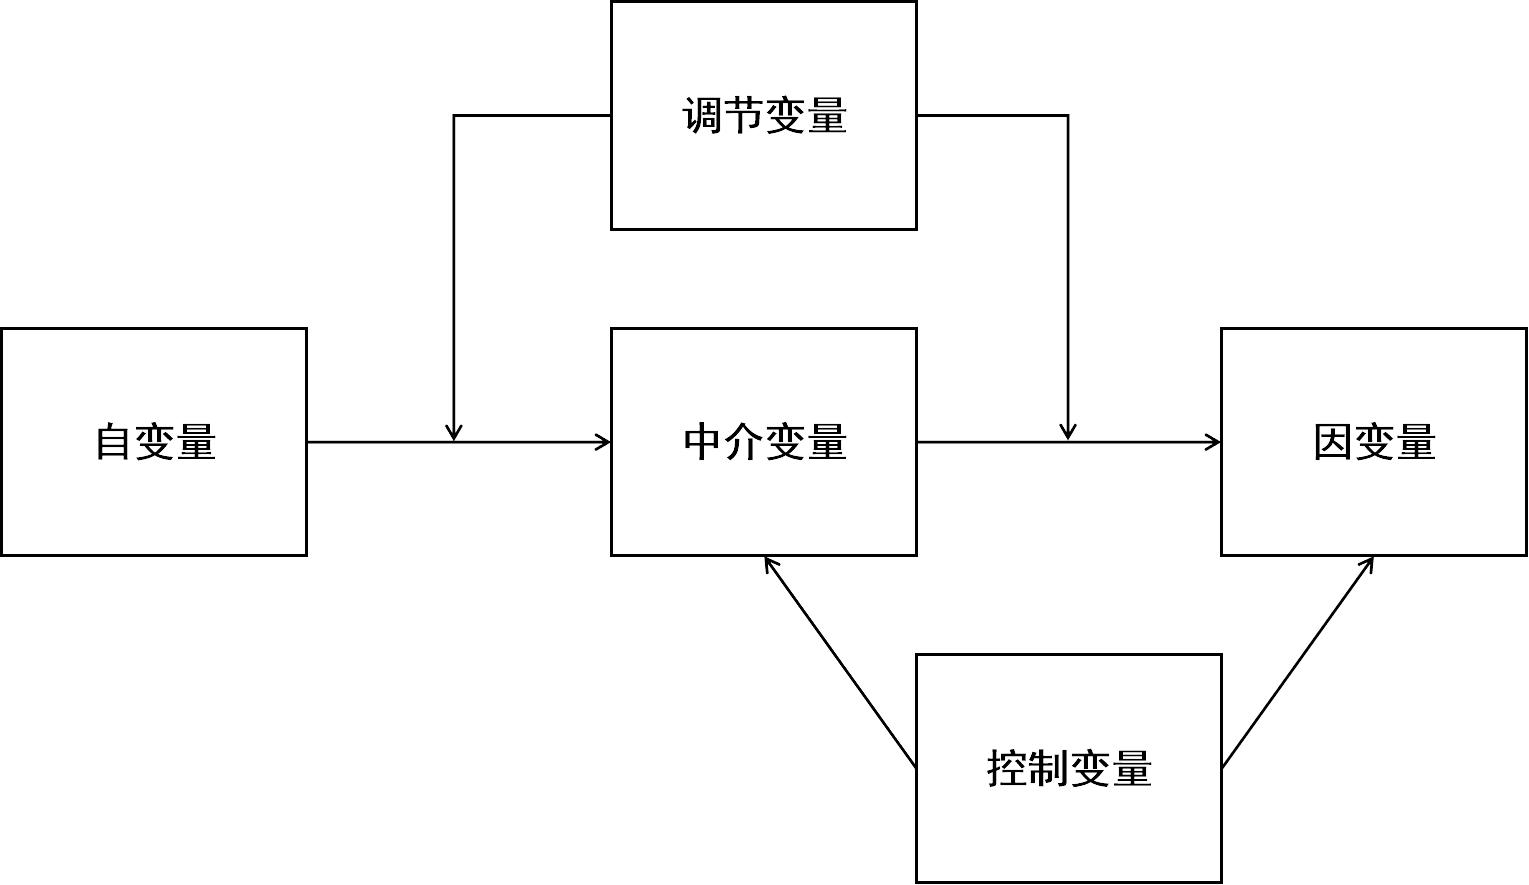
\includegraphics[width=0.5\textwidth]{image/f1.jpg}} % 用 \fbox 包裹图片
	\caption[变量间关系]{变量间关系}
	\label{fig:relation}
\end{figure}

需要明确的是,并非只有量化分析才需要用到变量思维,当代的政治科学名著中,如亨廷顿《变化社会中的政治秩序》,尽管没有用明确的假设H1一类指出,更没有用到统计分析,却仍然有一个完整的链条,总结一下大约是:

\begin{itemize}
	\item \textbf{自变}量:政治权威。
	\item \textbf{因变量}:政治发展。
	\item \textbf{中介变量}:政治秩序。
	\item \textbf{调节变量}:政党、领导人、社会结构等等。
	\item \textbf{控制变量}:一国的历史与现在(国家异质性)、国际体系变化等等。
\end{itemize}

\paragraph*{命题(proposition)}

是``对于一个概念的特征或多个概念间关系的陈述''。例如,``受教育水平更高的人相较于受教育水平更低的人文化消费更多''。

\paragraph*{假设(hypothesis)}

是命题的一种特殊形式,是为了得到逻辑的或经验的结论并加以检验而做的尝试性假说。假设通常是试探性的(也可以理解为实验性的),是为了被检验的目的而提出的严格的假设或建议。从这个角度来说,研究者通过提出待检验的假设,在抽象理论与经验事实之间建立了联结。

在大多数的社会科学研究中,由于研究者的主要目的大都可以归结为解释或说明不同变量之间的因果关系,因而,提出和检验有关变量间关系的假设成为科学研究和理论建构中不可或缺的环节。一般而言,假设有以下三种陈述方式:

\begin{itemize}
	\item
	\textbf{条件式陈述(conditional
		statement)}:其表达形式为``如果x,则y'',其中x代表前提或先决条件,y为结果。这种方式通常表示两个变量之间存在因果关系,但有时也指代相关关系。
	\item
	\textbf{差异式陈述(differential
		statement)}:其表达形式为``A组与B组在变量x上无(或有)差异''。在统计学中,无差异假设即``零假设''或``虚无假设''。
	\item
	\textbf{函数式陈述(functional
		statement)}:其数学表达式为y=f(x),即y是x的某种函数。它说明,如果变量x发生变化,则y也相应发生变化,反之亦然。函数式陈述在自然科学研究中较为常见,在以因果推断为方向的社会科学中也有增加的趋势。
\end{itemize}

\section{具体方法}

\subsection{研究对象}

\paragraph*{研究对象的选择与界定}

在开展研究时,明确研究对象是至关重要的第一步。研究对象的核心在于确定\textbf{分析单位},即研究的基本观测点。常见的分析单位包括:

\begin{enumerate}
	\item
	\textbf{个体层面}:以个人为研究对象,例如研究``个人收入差异的影响因素'',分析教育程度、工作经验等对个体收入的影响。
	\item
	\textbf{组织层面}:以企业、学校等组织为对象,比如探讨``企业创新效率的决定因素'',考察研发投入、人才结构等组织特征的影响。
	\item
	\textbf{国家层面}:以国家或地区为分析单位,如比较``不同产业政策对经济增长的影响'',需要收集各国政策和经济数据。
\end{enumerate}

需要警惕的是\textbf{生态学谬误},即错误地将高层次的分析结论直接推论到低层次单位。例如,用国家层面的收入不平等数据来推断个体幸福感,就可能犯这种错误——相对剥夺理论的最初研究就踏入其中\textsuperscript{\cite{4}}。

\paragraph*{数据类型}

研究设计时还需考虑\textbf{时空维度}的选择:

\begin{itemize}
	\item
	\textbf{截面数据}:捕捉同一时间点不同地区的状况,适合进行横向比较。例如2023年各省教育投入比较。
	\item
	\textbf{时序数据}:追踪同一地区不同时间的变化,适合趋势分析。如某省2000-2023年教育投入增长。
	\item
	\textbf{面板数据}:兼具截面和时序维度,能同时分析地区差异和时间变化。如全国31个省区市2010-2023年的教育投入数据。
\end{itemize}

\subsection{获取与分析数据}

找准所需数据的类型后,进入到数据分析方法的环节,以教育为主题为案例举例分析:

\paragraph*{观察法}

指研究者通过系统观察并记录教学过程中的现象来收集数据。例如,要研究教师提问方式对学生课堂参与度的影响,研究者可以在课堂上记录教师提问的类型(如开放式问题或封闭式问题)以及学生的回应情况(如举手次数、回答质量)。这种方法适用于自然教学环境下的行为研究,但存在两个主要挑战:一是观察者可能因主观判断产生偏差,二是若观察的课堂样本不足或仅限于特定班级,可能导致结论缺乏普遍性。

\paragraph*{实验法}

通过主动干预来验证教学方法的因果效应。典型操作是将学生随机分组,对实验组采用新教学方法(如项目式学习),对照组维持传统教学(如讲授式),学期末比较两组学生的成绩差异。例如,研究翻转课堂的效果时,随机分配部分班级使用课前视频学习+课堂讨论,另一部分采用常规授课,最终通过标准化测试评估学习成效。实验法的核心要求包括随机分组(确保学生基础水平均衡)、控制无关变量(如教材、课时一致),以及实验过程可重复验证。这种方法能直接证明教学方法的优劣,但可能因实验环境与真实课堂的差异而影响外部效度;在某些情况下,干预违背研究伦理而无法开展。

\paragraph*{准自然实验法}

当无法随机分组然后实验时,可利用教育政策或学校制度变化作为``自然实验''条件。例如,某地区推行``小班化教学改革'',研究者可比较改革前后同一学校学生的成绩变化,或对比改革校与非改革校的差异,使用双重差分法(DID)排除生源波动等因素干扰。另一种情况是,利用学校按分数线分班的规则(如``实验班''与普通班的分数线临界点),采用断点回归(RDD)分析教学差异对成绩的影响。这种方法依托现实教育场景,但需注意其他变量(如家庭支持、教师经验)可能混淆结论。

\subsection{总体与样本}

本部分参考《政治学与公共管理方法基础》,在讨论具体方法之前,我们需要明确几个核心概念:

\paragraph*{要素}

研究的基本分析单位,也是信息收集的对象,可以是一个人、一个班级、一所学校等。

\paragraph*{总体}

指研究对象的全部要素的集合,比如``某市所有高中生''就是一个总体。

\paragraph*{样本}

从总体中抽取的部分要素的集合,比如从该市随机选取的500名高中生。

\paragraph*{样本规模}

又称样本容量,指的是样本中包含的要素数量,比如上述的500人。

\paragraph*{样本代表性}

指样本在多大程度上能够反映总体的特征。一般来说,当样本的关键特征(如性别比例、成绩分布等)与总体越接近,代表性就越好。

\paragraph*{抽样}

无论选择哪种研究方法(质性研究还是量化研究),都要求我们从总体中抽取一定样本(否则真要累死),那具体怎么抽呢?抽样就是从研究总体中选择部分个体或要素作为样本的过程。要完成抽样,首先需要明确\textbf{抽样框}------也就是包含所有研究对象的清单或规则(比如全校学生名单),同时确定\textbf{抽样单位},即实际抽取的基本单位(比如个人、班级或学校)。

抽样方法主要分为两大类:\textbf{非概率抽样}和\textbf{概率抽样}。

\textbf{非概率抽样}不依赖随机原则,而是根据研究需求、主观判断或现实条件来选取样本,适合探索性研究或特殊案例分析。常见方法包括:

\begin{itemize}
	\item
	\textbf{方便抽样}:选最容易获取的样本(比如就近调查自己班的学生);
	\item
	\textbf{目标抽样}:按特定标准选取(比如只研究成绩前10\%的学生);
	\item
	\textbf{滚雪球抽样}:通过已有样本推荐新样本(比如通过少数留学生找到更多留学生受访者);
	\item
	\textbf{配额抽样}:按比例匹配总体特征(比如男女各抽50人);
	\item
	\textbf{典型案例抽样}(选最具代表性的案例)、\textbf{极端案例抽样}(选表现异常好或差的个体)、\textbf{负面案例抽样}(故意选不符合理论的案例)等。
\end{itemize}

\textbf{概率抽样}则严格遵循随机原则,确保每个个体有已知的、非零的被抽中概率,适合需要统计推断的研究。常用方法有:

\begin{itemize}
	\item
	\textbf{简单随机抽样}:像抽签一样完全随机选取;
	\item
	\textbf{系统抽样}:按固定间隔抽取(如每第10个学生);
	\item
	\textbf{分层抽样}:先按特征分组(如年级),再在各层内随机抽;
	\item
	\textbf{整群抽样}:随机抽取完整群体(如抽几个班级而非个别学生);
	\item
	\textbf{多阶抽样}:分多个阶段逐步缩小范围(如先抽城市,再抽学校,最后抽班级)。
\end{itemize}

\paragraph*{抽样误差}

抽样过程不可避免地会产生\textbf{误差},即样本统计量(如样本平均分)与总体参数(如全市高中生真实平均分)之间的差异。这种误差是随机产生的(\textbf{无法根除}),但可以通过科学的抽样方法和适当的样本规模来降低(\textbf{但不能躺平})。

选择抽样方法时,非概率抽样灵活但可能偏差大,概率抽样科学但成本高。实际研究中常结合使用,比如先滚雪球找到目标群体,再用分层抽样确保代表性。

\subsection{得出结论}

本部分参考《政治学与公共管理方法基础》、《比较政治学:理论与方法》\textsuperscript{\cite{5}}和《比较政治中的议题与方法》\textsuperscript{\cite{6}},为了确保我们得出的是一个流程科学结果合理的结论,我们还需要反复考量如下要求:

\paragraph*{控制变异}

在社会科学研究中,控制变异是确保研究结论可靠性的关键环节。研究者需要通过系统的方法来最大化研究变量的差异,控制干扰因素,并减少测量误差。

\begin{enumerate}
	\item \textbf{最大化系统差异}:指由于自变量变化而引起的因变量的变化幅度要达到最大(变化越大越能找到规律)。明确研究问题,确定最佳的自变量和因变量,同时应该考虑到自变量和因变量的所有情况,并选定合理的样本范围。
	\item \textbf{控制外生变量} :控制外生变量主要有三种方法:
	
	\begin{itemize}
		\item \textbf{纳入法}:将可能影响结果的重要变量纳入分析模型。\textbf{核心变量}(如政策实施年份、受教育年限)必须包含,同时要控制\textbf{人口统计学变量}(如年龄、性别)和\textbf{环境变量}(如行业类型、宏观变量等)。
		\item \textbf{非纳入法}:通过研究设计来控制变量。\textbf{同质法}即没有外生变量不一致导致的误差(一般这样只能找到有限个特征相同,不能保证完全相同,用得很少);\textbf{随机分配法}确保\textbf{实验组}和\textbf{对照组}在各方面均衡(概率抽样);\textbf{配对法}则根据相似特征(如经济发展水平、人口规模)来匹配比较对象。
	\end{itemize}
	\item
	\textbf{最小化误差差异}:测量误差的控制至关重要。采用标准化测量工具(如Likert五级量表)可以提高数据一致性。同时,通过多源数据交叉验证,也可以显著提升数据的准确性和可靠性。
\end{enumerate}

\paragraph*{研究效度}

\begin{itemize}
	\item
	\textbf{构念效度}:指一个构念能够正确反映其所要表达、描述或测量对象内容和特征的程度,或者也可以定义为一个构念表达、描述和测量的精确性。
	\item
	\textbf{内部效度}:指基于特定研究对象而得出的结论本身符合特定研究对象实际情况的程度;而对探求精确因果性关系的定量研究而言,则是基于特定研究对象得出的变量(或构念)间因果关系的推论符合特定研究对象实际情况的程度,也即其因果关系推论对特定对象本身而言的可信度。
	\item
	\textbf{外部效度}:指将从特定研究对象得出的研究结论推广到具有不同分析单位、时间维度、研究区域、研究层次、研究尺度等的其他研究对象的可信度。
	\item
	\textbf{统计结论效度}:指通过统计检验对假设关系进行解释的可信度。
\end{itemize}

需要说明的是,这四种效度常互相制衡(如提高内部效度可能损害外部效度);而追求统计结论效度实际上也可能犯了构念效度的损伤(试变量试到跑题)。

\section{定性与定量的融合}

上文虽然是定量分析的范式,但定性亦可参照一二,诸多时候定量分析的理论渊源实际上来自定性,更遑论KKV(加里·金/Gary King、罗伯特·基欧汉/Robert O. Keohane、悉尼·维巴/Sidney Verba)三人经典的《\emph{Designing Social Inquiry}》中早已有详尽的解释(其繁体版译本名为《好研究如何設計?:用量化邏輯做質化研究》)。

对这一部分的理解有助于我们理解计量经济学的开端、发展与变革,从而更好理解结构计量的设计转向。值得注意的是,KKV倡导的``量化逻辑''并非要将质性研究简单数字化,而是强调研究设计中的因果推断逻辑必须严谨。这种思想与Angrist等人提出的``可信性革命''遥相呼应,二者都要求研究者超越方法论的二元对立,在保持方法适切性的前提下实现优势互补。当处理异质性处理效应时,定性访谈揭示的个体决策过程往往能修正定量模型的设定偏误;而大样本数据分析又能检验质性研究发现的外部效度。

\newpage
\thispagestyle{empty}
\begin{thebibliography}{99}
	\bibitem{1}
	董晨宇 \ 等,《拆论文:从精读中领悟学术写作》,重庆大学出版社
	
	\bibitem{2}
	杨立华 \ 等,《政治学与公共管理研究方法基础》,北京大学出版社
	
	\bibitem{3}
	马亮,《学术祛魅:实证研究十讲》,中国人民大学出版社
	
	\bibitem{4}
	王正绪 \ 等,《比较政治学》,复旦大学出版社
	
	\bibitem{5}
	B.盖伊·彼得斯,《比较政治学:理论与方法》,上海人民出版社
	
	\bibitem{6}
	托德·兰德曼 \ 等,《比较政治中的议题与方法》,上海人民出版社
	
\end{thebibliography}
\chapter{定量分析的数理基础}

\section{数学}
定量研究对于不少文科专业的同学来说最关键的一个门槛便是理解数学公式,好在笔者本人也是文科专业出身,写这一部分足够契合(水平也菜)。

本文介绍了因果推断中常用的数学基础,包括微积分、线性代数、概率与分布、以及统计推断等内容。这些基础知识为理解和应用因果推断方法提供了必要的数学工具。

\subsection{微积分}

\paragraph*{函数}
在数学中,函数是一种特殊的关系,它将一个集合中的每个元素(\textbf{自变量})映射到另一个集合中的唯一元素(\textbf{因变量})。函数可以用多种方式表示,包括解析式、图像、表格和算法等。函数的概念在微积分中至关重要,因为微积分的主要研究对象就是函数的变化率和累积量。

\paragraph*{导数}
一元函数 $ y = f(x) $ 的一阶导数定义为:
\begin{equation}
\frac{\mathrm{d}y}{\mathrm{d}x} \equiv f'(x) \equiv \lim_{\Delta x \to 0} \frac{\Delta y}{\Delta x} \equiv \lim_{\Delta x \to 0} \frac{f(x + \Delta x) - f(x)}{\Delta x}
\end{equation}

\noindent 其几何意义是函数在某点的切线斜率。二阶导数定义为:
\begin{equation}
\frac{\mathrm{d}^2y}{\mathrm{d}x^2} \equiv f''(x) \equiv [f'(x)]'\equiv \frac{\mathrm{d}\left(\frac{\mathrm{d}y}{\mathrm{d}x}\right)}{\mathrm{d}x}
\end{equation}
\noindent 二阶导数反映了函数图像切线斜率的变化率,描述了曲线的弯曲程度,这一性质在数学中被称为\textbf{曲率(curvature)}。在经济学中,我们一般默认二阶导数恒为正或负值。

\begin{figure}[ht]
	\centering
	\fbox{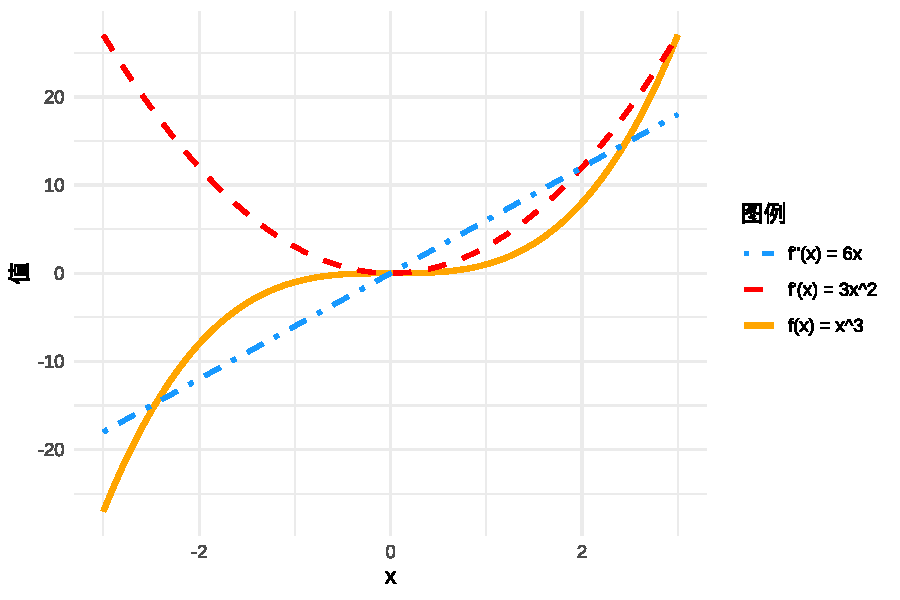
\includegraphics[width=0.5\textwidth]{image/f2.pdf}}
	\caption{函数 $f(x) = x^3$ 与其一阶、二阶导数}
\end{figure}

\paragraph*{偏导数}
偏导数是多元函数对其中一个变量的导数,而将其他变量视为常数。例如,对于二元函数 \( y = f(x, z) \),其对 \( x \) 的偏导数定义为:
\begin{equation}
	\frac{\partial y}{\partial x} \equiv \lim_{\Delta x \to 0} \frac{f(x + \Delta x, z) - f(x, z)}{\Delta x}
\end{equation}
\noindent 类似地,对 \( z \) 的偏导数为:
\begin{equation}
	\frac{\partial y}{\partial z} \equiv \lim_{\Delta z \to 0} \frac{f(x, z + \Delta z) - f(x, z)}{\Delta z}
\end{equation}
\noindent 偏导数在经济学中有着广泛的应用,例如在效用函数和生产函数中,偏导数分别表示商品和生产要素的边际效应。

\paragraph*{基本求导规则}

\begin{itemize}
	\item 线性法则:$(cf)' = c f'$, 其中$c$为常数;
	\item 乘法法则:$(fg)' = f'g + fg'$;
	\item 除法法则:$\left(\dfrac{f}{g}\right)' = \dfrac{f'g - fg'}{g^2}$;
	\item 链式法则:$(f(g(x)))' = f'(g(x)) \cdot g'(x)$。
\end{itemize}

\begin{table}[h]
	\centering
	\caption{常见函数的导数公式}
	\renewcommand{\arraystretch}{2}
	\begin{tabularx}{\linewidth}{>{\centering\arraybackslash}X >{\centering\arraybackslash}X}
		\toprule
		函数 & 导数 \\
		\midrule
		常数 $c$         & $0$ \\
		$x^n$            & $n x^{n-1}$ \\
		$\sin x$         & $\cos x$ \\
		$\cos x$         & $-\sin x$ \\
		$e^x$            & $e^x$ \\
		$a^x$            & $a^x \ln a$ \\
		$\ln x$          & $\dfrac{1}{x}$ \\
		$\log_a x$       & $\dfrac{1}{x \ln a}$ \\
		$\tan x$         & $\sec^2 x$ \\
		\bottomrule
	\end{tabularx}
\end{table}

\paragraph*{洛必达法则}
洛必达法则的核心思想是通过分子分母分别求导,解决$\frac{0}{0}$或$\frac{\infty}{\infty}$型不定式极限问题:
\begin{equation}
	\lim_{x \to c} \frac{f(x)}{g(x)} = \lim_{x \to c} \frac{f'(x)}{g'(x)} \quad \text{(若满足条件)}
\end{equation}
适用条件包括:极限形式为$\frac{0}{0}$或$\frac{\infty}{\infty}$,$f(x), g(x)$在$c$的去心邻域内可导且$g'(x) \neq 0$,求导后极限存在或为无穷。

\vspace{0.8em} % 手动调整间距

\begin{example}
\noindent 证明 $\lim\limits_{x\to+\infty}\left(1+\frac{1}{x}\right)^{x}=e$
	\begin{flushleft}
		\textbf{证明思路}:通过取对数转换,构造$\frac{0}{0}$型极限,应用洛必达法则求解。
	\end{flushleft}
	\begin{flushleft}	
		\textbf{证明步骤:}
	\end{flushleft}
	\begin{enumerate}
		\item 设 $y = \left(1+\frac{1}{x}\right)^x$,取对数得 $\ln y = x\ln\left(1+\frac{1}{x}\right)$
		\item 令 $t=\frac{1}{x}$,转化为 $\lim\limits_{t\to 0^+}\frac{\ln(1+t)}{t}\ \left(\frac{0}{0}\text{型}\right)$
		\item 应用洛必达法则:
		$$
		\lim_{t\to 0^+}\frac{\ln(1+t)}{t} \overset{\text{L'H}}{=} \lim_{t\to 0^+}\frac{1/(1+t)}{1} = 1
		$$
		\item 还原得 $\lim\limits_{x\to+\infty}\ln y =1 \ \Rightarrow\ \lim\limits_{x\to+\infty} y = e^1 = e$
	\end{enumerate}
\end{example}

\paragraph*{一元最优化}
最小二乘法(OLS)和最大似然估计(MLE)都是最优化问题。无约束的一元最优化问题中,最大化问题的一阶条件为$f'(x^*) = 0$,二阶条件为$f''(x^*) \leq 0$;最小化问题的一阶条件同样为$f'(x^*) = 0$,二阶条件为$f''(x^*) \geq 0$。

\paragraph*{多元最优化}

考虑无约束的多元最大化问题:
\begin{equation}
	\max_x f(x) = f(x_1, x_2, \ldots, x_n)
\end{equation}

\noindent 其一阶条件要求在最优值 $x^*$ 处,所有偏导数均为0:

\begin{equation}
	\frac{\partial f}{\partial x_i}(x^*) = 0 \quad \text{for all } i = 1, 2, \ldots, n
\end{equation}

\noindent 该条件称为\textbf{一阶必要条件},在满足一阶条件的基础上,其充分条件为:

\paragraph*{Hessian条件}

记函数的Hessian矩阵为:
\begin{equation}
	\mathbf{H(x)} = \begin{bmatrix}
		\frac{\partial^2 f}{\partial x_1^2} & \frac{\partial^2 f}{\partial x_1 \partial x_2} & \cdots & \frac{\partial^2 f}{\partial x_1 \partial x_n} \\
		\frac{\partial^2 f}{\partial x_2 \partial x_1} & \frac{\partial^2 f}{\partial x_2^2} & \cdots & \frac{\partial^2 f}{\partial x_2 \partial x_n} \\
		\vdots & \vdots & \ddots & \vdots \\
		\frac{\partial^2 f}{\partial x_n \partial x_1} & \frac{\partial^2 f}{\partial x_n \partial x_2} & \cdots & \frac{\partial^2 f}{\partial x_n^2}
	\end{bmatrix}
\end{equation}

\begin{itemize}
	\item 若 $\mathbf{H(x^*)}$ 是\textbf{负定矩阵},则 $x^*$ 是局部极大值点。
	\item 若 $\mathbf{H(x^*)}$ 是\textbf{正定矩阵},则 $x^*$ 是局部极小值点。
	\item 若 $\mathbf{H(x^*)}$ \textbf{半正定或半负定},则可能为鞍点或边界情况。
\end{itemize}
\vspace{0.8em} % 手动调整间距

\noindent 其中,负定和正定矩阵的判定方法可通过特征值符号判断。

\begin{figure}[ht]
	\centering
	\fbox{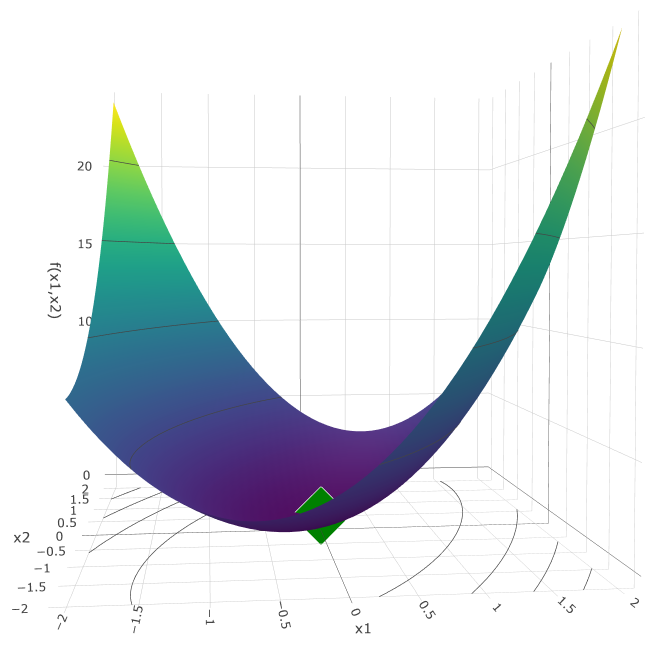
\includegraphics[width=0.5\textwidth]{image/divers.png}}
	\caption{一个抽象的多元最优化示意图}
\end{figure}

\subsection{线性代数}

\paragraph*{矩阵}
将 \( m \times n \) 个实数排列成如下矩形阵列:
\begin{equation}
\mathbf{A} = 
\begin{bmatrix}
	a_{11} & \cdots & a_{1n} \\
	\vdots & \ddots & \vdots \\
	a_{m1} & \cdots & a_{mn}
\end{bmatrix}
\end{equation}
称 \( \mathbf{A} \) 为 \( m \times n \) 级矩阵(matrix),其中:
\begin{itemize}
	\item \( m \):行数(row dimension)
	\item \( n \):列数(column dimension)
\end{itemize}

\noindent 元素 \( a_{ij} \) 表示第 \( i \) 行、第 \( j \) 列的元素。记法:\( \mathbf{A_{m \times n}} \) 或者 \( (a_{ij})_{m \times n} \)。若所有元素均为 0,则称为零矩阵(zero matrix),记作 \( \bm{0} \)。

\paragraph*{矩阵的转置}
将矩阵 \( \mathbf{A} = (a_{ij}) \) 的第 \( i \) 行变为第 \( i \) 列,得到其转置矩阵 \( \mathbf{A'} \),维度为 \( n \times m \):

\begin{equation}
	\mathbf{(A')_{ij}} = \mathbf{(A)_{ji}}
\end{equation}

\begin{itemize}
	\item 若 \( \mathbf{A} \) 是对称矩阵,则 \( \mathbf{A'} = \mathbf{A} \)
	\item 转置的转置还原:\( \mathbf{(A')'} = \mathbf{A} \)
\end{itemize}

\paragraph*{方阵}
当 \( m = n \) 时,矩阵 \( \mathbf{A} \) 称为 \( n \) 阶方阵:
\begin{equation}
\mathbf{A} = 
\begin{bmatrix}
	a_{11} & \cdots & a_{1n} \\
	\vdots & \ddots & \vdots \\
	a_{n1} & \cdots & a_{nn}
\end{bmatrix}
\end{equation}

\noindent 主对角线元素为\( a_{11}, a_{22}, \ldots, a_{nn} \)。
\begin{flushleft}
	常见类型有:
\end{flushleft}
\begin{itemize}
	\item 对称矩阵:\( a_{ij} = a_{ji} \)。
	\item 对角矩阵:非主对角线元素全为 0。
	\item 单位矩阵 \( \mathbf{I_n} \):主对角线为 1,其余为 0。
\end{itemize}

\noindent 上述三种类型的矩阵限制条件逐项增加,可以看到单位矩阵一定是对角矩阵和对称矩阵;单位矩阵 \( \mathbf{I_n} \) 在矩阵运算中作用类似于数字 1。

\paragraph*{行列式}
\begin{flushleft}
	\textbf{定义}:方阵的一个标量值函数
\end{flushleft}

\begin{itemize}
	\item 记法:$\det(\mathbf{A})$ 或 $|\mathbf{A}|$
	\item 对于 $n \times n$ 矩阵 $\mathbf{A} = (a_{ij})$:
	\begin{equation}
		\det(\mathbf{A}) = \sum_{\sigma \in S_n} \operatorname{sgn}(\sigma) \prod_{i=1}^n a_{i,\sigma(i)}
	\end{equation}
	\noindent 其中:
	\begin{itemize}
		\item $S_n$ 是 $\{1, \ldots, n\}$ 的所有排列集合
		\item $\operatorname{sgn}(\sigma)$ 是排列符号函数(偶排列为 $+1$,奇排列为 $-1$)
	\end{itemize}
\end{itemize}

\paragraph*{行列式的求解} 

\begin{flushleft}
	\textbf{定义:}
\end{flushleft}

\begin{itemize}
	\item 排列中``逆序对''的数量
	\item 举例:123(1<2<3,0),213(2>1<3,1),321(3>2>1,3)
\end{itemize}

\begin{flushleft}
	\textbf{三阶行列式展开:}
\end{flushleft}

\begin{equation}
\mathbf{D_3} = \sum (-1)^t a_{1p_1}a_{2p_2}a_{3p_3}
\end{equation}

\begin{itemize}
	\item $p_1p_2p_3$: $1,2,3$ 的排列
	\item $t$: 排列的逆序数
	\item 共6项(例如:排列 $213$ 对应 $-a_{12}a_{21}a_{33}$)
\end{itemize}

\paragraph*{n阶行列式}
\begin{equation}
	\mathbf{D_n} = \sum (-1)^t a_{1p_1} a_{2p_2} \cdots a_{np_n}
\end{equation}
\begin{itemize}
	\item $p_1 p_2 \cdots p_n$: $1$ 到 $n$ 的排列
	\item $t$: 排列的逆序数
	\item 总共 $n!$ 项(如:3阶有6项,4阶有24项)
\end{itemize}

\vspace{0.7em}
\begin{example}
	
	\noindent 设矩阵:
		\begin{equation}
		\mathbf{A} = \begin{bmatrix}
			1 & 2 & 3 \\
			4 & 5 & 6 \\
			7 & 8 & 9
		\end{bmatrix}
		\end{equation}
		
	\noindent 行列式展开:
		\begin{equation}
		\det(\mathbf{A}) = 
		1 \cdot 5 \cdot 9 + 2 \cdot 6 \cdot 7 + 3 \cdot 4 \cdot 8
		- 3 \cdot 5 \cdot 7 - 2 \cdot 4 \cdot 9 - 1 \cdot 6 \cdot 8
		\end{equation}
		
	\noindent 计算得:
		\begin{equation}
		\det(\mathbf{A}) = 45 + 84 + 96 - 105 - 72 - 48 = 0
		\end{equation}
		
	\noindent 所以:$\det(\mathbf{A}) = 0$
\end{example}

\paragraph*{向量}

\begin{flushleft}
	\textbf{定义}:若 \( m = 1 \),矩阵 \( \mathbf{A} \) 称为 \( n \) 维行向量(row vector);若 \( n = 1 \),则称为 \( m \) 维列向量(column vector)。向量是矩阵的特例。
\end{flushleft}


\begin{flushleft}
	设列向量:
\end{flushleft}

\begin{equation}
\mathbf{a} = \begin{bmatrix} a_1 \\ \vdots \\ a_n \end{bmatrix},\quad
\mathbf{b} = \begin{bmatrix} b_1 \\ \vdots \\ b_n \end{bmatrix}
\end{equation}

\begin{flushleft}
	它们的内积(点乘)定义为:
\end{flushleft}

\begin{equation}
	\begin{aligned}
		\mathbf{a}'\mathbf{b} &\equiv 
		\begin{pmatrix} a_1 & \cdots & a_n \end{pmatrix}
		\begin{pmatrix} b_1 \\ \vdots \\ b_n \end{pmatrix} \\
		&= a_1 b_1 + \cdots + a_n b_n = \sum_{i=1}^{n} a_i b_i
	\end{aligned}
\end{equation}

\begin{flushleft}
	\textbf{向量正交性}
\end{flushleft}


\begin{flushleft}
	\textbf{定义}:若 \( \mathbf{a}'\mathbf{b} = 0 \),称 \( \mathbf{a} \) 与 \( \mathbf{b} \) 正交,即在 \( n \) 维空间中相互垂直。任何形如 $\sum_{i=1}^{n} a_i b_i$ 的乘积求和,都可以很方便地写为向量内积 $a'b$ 的形式。特别地,平方和 $\sum_{i=1}^{n} a_i^2$ 可写为 $\mathbf{a'a}$:
\end{flushleft}


\begin{equation}
	\begin{aligned}
		\mathbf{a'a} = \begin{pmatrix} a_1 & a_2 & \cdots & a_n \end{pmatrix}
		\begin{pmatrix}
			a_1 \\
			a_2 \\
			\vdots \\
			a_n
		\end{pmatrix}
		\equiv a_1^2 + a_2^2 + \cdots + a_n^2 = \sum_{i=1}^{n} a_i^2
	\end{aligned}
\end{equation}

\paragraph*{矩阵加法与数乘}
\begin{flushleft}
	\textbf{矩阵加法}:若 \( \mathbf{A} = (a_{ij}) \) 和 \( \mathbf{B} = (b_{ij}) \) 是同维矩阵,则:
\end{flushleft}

\begin{equation}
\mathbf{A} + \mathbf{B} = (a_{ij} + b_{ij})
\end{equation}
\begin{flushleft}
	\textbf{数乘}:实数 \( k \) 与矩阵 \( \mathbf{A} = (a_{ij})_{m \times n} \) 的数乘为:
\end{flushleft}

\begin{equation}
k\mathbf{A} = (k a_{ij})
\end{equation}

\begin{flushleft}
	矩阵的加法满足以下规则:
\end{flushleft}

\begin{enumerate}
	\item $\mathbf{A} + \mathbf{0} = \mathbf{A}$ \hfill (加上零矩阵不改变矩阵)
	\item $\mathbf{A} + \mathbf{B} = \mathbf{B} + \mathbf{A}$ \hfill (加法交换律)
	\item $(\mathbf{A} + \mathbf{B}) + \mathbf{C} = \mathbf{A} + (\mathbf{B} + \mathbf{C})$ \hfill (加法结合律)
	\item $(\mathbf{A} + \mathbf{B})' = \mathbf{A}' + \mathbf{B}'$ \hfill (转置为线性运算)
\end{enumerate}

\paragraph*{矩阵乘法}
设 \( \mathbf{A} \) 为 \( m \times n \) 矩阵,\( \mathbf{B} \) 为 \( n \times q \) 矩阵,则乘积 \( \mathbf{AB} \) 的元素定义为:
\begin{equation}
	(\mathbf{AB})_{ij} \equiv 
	\begin{pmatrix}
		a_{i1} & a_{i2} & \cdots & a_{in}
	\end{pmatrix}
	\begin{pmatrix}
		b_{1j} \\
		b_{2j} \\
		\vdots \\
		b_{nj}
	\end{pmatrix}
	=
	\sum_{k=1}^{n} a_{ik} b_{kj}
\end{equation}
\textbf{注意}:矩阵乘法不满足交换律($ AB \neq BA $)。

\begin{flushleft}
	矩阵的乘法满足以下规则:
\end{flushleft}

\begin{enumerate}
	\item $\mathbf{IA} = \mathbf{A}$, $\mathbf{AI} = \mathbf{A}$ \hfill (乘以单位矩阵不改变矩阵)
	\item $(\mathbf{AB})\mathbf{C} = \mathbf{A}(\mathbf{BC})$ \hfill (乘法结合律)
	\item $\mathbf{A}(\mathbf{B}+\mathbf{C}) = \mathbf{AB} + \mathbf{AC}$ \hfill (乘法分配律)
	\item $(\mathbf{AB})' = \mathbf{B}'\mathbf{A}'$, $(\mathbf{ABC})' = \mathbf{C}'\mathbf{B}'\mathbf{A}'$ \hfill (转置与乘积的混合运算)
\end{enumerate}

\paragraph*{线性方程组}

\begin{flushleft}
	\textbf{定义}:考虑以下由 $n$ 个方程、$n$ 个未知数构成的线性方程组
\end{flushleft}

\vspace{-0.5em}
\begin{equation}
	\left\{
	\begin{aligned}
		a_{11}x_1 + \cdots + a_{1n}x_n &= b_1 \\
		\vdots\quad\ \ &\vdots \\
		a_{n1}x_1 + \cdots + a_{nn}x_n &= b_n
	\end{aligned}
	\right.
\end{equation}

\begin{flushleft}
	其中,$(x_1, \ldots, x_n)$ 为未知数,可将上式写为:
\end{flushleft}

\vspace{-0.2em}
\begin{equation}
	\underbrace{
		\begin{pmatrix}
			a_{11} & \cdots & a_{1n} \\
			\vdots & \ddots & \vdots \\
			a_{n1} & \cdots & a_{nn}
		\end{pmatrix}
	}_{\mathbf{A}}
	\begin{pmatrix}
		x_1 \\ \vdots \\ x_n
	\end{pmatrix}
	=
	\begin{pmatrix}
		b_1 \\ \vdots \\ b_n
	\end{pmatrix}
	\quad \Rightarrow \quad \mathbf{Ax} = \mathbf{b}
\end{equation}

\begin{flushleft}
	直观上,如果可将此方程左边的方阵 $\mathbf{A}$ ``除'' 到右边去,则可得到 $\mathbf{x}$ 的解。为此,引入\textbf{逆矩阵}的概念。
\end{flushleft}


\paragraph*{逆矩阵}
\begin{flushleft}
	\textbf{定义}:设 $\mathbf{A}$ 为 $n$ 阶方阵。若存在方阵 $\mathbf{B}$,使得  
\end{flushleft}

\vspace{-0.5em}
\begin{equation}
\mathbf{AB} = \mathbf{BA} = \mathbf{I_n}
\end{equation} 

\begin{flushleft}
	则称 $\mathbf{A}$ 可逆(或非退化),$\mathbf{B}$ 是其逆矩阵,记作 $\mathbf{A^{-1}}$。  
	可逆的充要条件是 $|\mathbf{A}| \neq 0$,且逆矩阵唯一。假设方程中的矩阵 $\mathbf{A}$ 可逆,则在该方程两边同时左乘其逆矩阵 $\mathbf{A^{-1}}$ 可得:
\end{flushleft}

\vspace{-0.5em}
\begin{equation}
	\mathbf{A^{-1}}\mathbf{A}\mathbf{x} = \mathbf{A^{-1}}\mathbf{b} \Rightarrow \mathbf{I}\mathbf{x} = \mathbf{A^{-1}}\mathbf{b} \Rightarrow \mathbf{x} = \mathbf{A^{-1}}\mathbf{b}
\end{equation}

\begin{flushleft}
	矩阵求逆满足以下规则:
\end{flushleft}
\begin{enumerate}
	\item $(\mathbf{A^{-1})'} = (\mathbf{A')^{-1}}$ \hfill (求逆与转置可交换次序)
	\item $(\mathbf{AB)^{-1}} = \mathbf{B^{-1}}\mathbf{A^{-1}}$
	\item $(\mathbf{ABC)^{-1}} = \mathbf{C^{-1}}\mathbf{B^{-1}}\mathbf{A^{-1}}$ \hfill (求逆与乘积的混合运算)
\end{enumerate}

\paragraph*{矩阵的秩}
向量组的线性相关性
\begin{itemize}
	\item 对于两个$n$维列向量$\mathbf{a}_1$与$\mathbf{a}_2$:若$\mathbf{a}_1$是$\mathbf{a}_2$的固定倍数,则向量组$\{\mathbf{a}_1, \mathbf{a}_2\}$中只有一个向量真正含有信息。
	
	\item $K$个$n$维向量$\{\mathbf{a}_1, \mathbf{a}_2, \cdots, \mathbf{a}_k\}$,若存在不全为零的标量$c_1, c_2, \cdots, c_k$使得:
	\begin{equation}
		c_1 \mathbf{a}_1 + c_2 \mathbf{a}_2 + \cdots + c_k \mathbf{a}_k = \mathbf{0}
	\end{equation}
\end{itemize}

\begin{flushleft}
则称向量组线性相关(linearly dependent)。若仅当$c_1 = c_2 = \cdots = c_k = 0$时上式成立,则称线性无关(linearly independent)
\end{flushleft}



\begin{flushleft}
向量组的秩:极大线性无关部分组所含向量的个数。
\end{flushleft}

\begin{itemize}
	\item 列秩(column rank):列向量组的秩
	\item 行秩(row rank):行向量组的秩
	\item 重要性质:行秩 = 列秩,统称为矩阵的秩(matrix rank)
	\item 满列秩:若$m \times n$矩阵的列秩等于$n$
\end{itemize}

\paragraph*{行阶梯形法}:	通过初等行变换将矩阵化为行阶梯形,非零行数即为秩。

\vspace{0.8em} % 手动调整间距

\begin{example}
	计算矩阵 $ B = \begin{bmatrix} 1 & 2 & 3 \\ 4 & 5 & 6 \\ 7 & 8 & 9 \end{bmatrix} $ 的秩
	
	\vspace{0.5em}
	\begin{flushleft}	
	\textbf{步骤 1:消除第一列下方元素}
	
	初始矩阵:
	\begin{equation}
		\begin{bmatrix} 
			1 & 2 & 3 \\ 
			4 & 5 & 6 \\ 
			7 & 8 & 9 
		\end{bmatrix}
	\end{equation}
	
	执行初等行变换:
	\begin{align*}
		R_2 &\leftarrow R_2 - 4R_1 \\
		R_3 &\leftarrow R_3 - 7R_1
	\end{align*}
	
	结果为:
	\begin{equation}
		\begin{bmatrix} 
			1 & 2 & 3 \\ 
			0 & -3 & -6 \\ 
			0 & -6 & -12 
		\end{bmatrix}
	\end{equation}
	
	\textbf{步骤 2:消除第二列下方元素}
	
	继续对当前矩阵进行变换:
	\begin{equation}
		\begin{bmatrix} 
			1 & 2 & 3 \\ 
			0 & -3 & -6 \\ 
			0 & -6 & -12 
		\end{bmatrix}
	\end{equation}
	
	执行变换:
	\begin{align*}
		R_3 \leftarrow R_3 - 2R_2
	\end{align*}
	
	得到行阶梯形矩阵:
	\begin{equation}
		\begin{bmatrix} 
			1 & 2 & 3 \\ 
			0 & -3 & -6 \\ 
			0 & 0 & 0 
		\end{bmatrix}
	\end{equation}
	
	非零行有 2 行,因此 $ r(B) = 2 $。
	\end{flushleft}

\end{example}

\paragraph*{多重共线性与研究设计(KKV)}
\begin{flushleft}
	\textbf{定义}:一个解释变量可被其他变量预测,影响对各自独立效应的识别(不依赖线性假设)。
\end{flushleft}

\begin{flushleft}
	\textbf{问题实例}(军备合作):
\end{flushleft}
\begin{itemize}
	\item 假设1:大小不同的国家更易合作。
	\item 假设2:不相邻国家更易合作。
	\item 若观察值仅限于``大小不同且相邻''或``大小相同但不相邻'',则无法区分两个变量的影响。
\end{itemize}

\begin{flushleft}
	\textbf{解决方案}:
\end{flushleft}
\begin{itemize}
	\item 收集更多理论相关案例(如大小相同又邻近的国家)。
	\item 或从其他分析层次寻找可观测意涵。
\end{itemize}

\paragraph*{二次型与正定性}
对于对称矩阵 $ \mathbf{A} $,二次型定义为:
\begin{equation}
f(\mathbf{x}) = \mathbf{x}' \mathbf{A} \mathbf{x} = \sum_{i=1}^n \sum_{j=1}^n a_{ij} x_i x_j
\end{equation}
\textbf{分类}:
\[
\begin{cases}
	\mathbf{x}' \mathbf{A} \mathbf{x} > 0, \quad \forall \mathbf{x} \neq 0 & \text{正定矩阵} \\
	\mathbf{x}' \mathbf{A} \mathbf{x} \geq 0, \quad \forall \mathbf{x} \neq 0 & \text{半正定矩阵} \\
	\mathbf{x}' \mathbf{A} \mathbf{x} < 0, \quad \forall \mathbf{x} \neq 0 & \text{负定矩阵} \\
	\mathbf{x}' \mathbf{A} \mathbf{x} \leq 0, \quad \forall \mathbf{x} \neq 0 & \text{半负定矩阵}
\end{cases}
\]
\textbf{应用}:计量经济学中常用 $ \mathbf{x}' [Var(\mathbf{x})]^{-1} \mathbf{x} $ 度量标准化距离。

\section{统计学}
	
\subsection{概率与分布}

\paragraph*{无条件概率}

\begin{flushleft}
\textbf{定义}:无条件概率是概率论中最基础的概念之一,表示事件$A$发生的概率,记作$P(A)$。例如,我们可以研究股市崩盘的概率。无条件概率的特点是独立于其他事件,即不考虑任何其他事件的影响。
\end{flushleft}
	
\paragraph*{条件概率}
\begin{flushleft}
	条件概率的数学定义为:
\end{flushleft}

\begin{equation}
	P(A\mid B)=\frac{P(AB)}{P(B)}
\end{equation}
其中$AB=A\cap B$表示事件$A$和$B$同时发生的情况(例如``太阳雨''事件)。一个典型的应用场景是:已知经济衰退时,计算股市崩盘的概率。


\paragraph*{独立事件}
\begin{flushleft}
	对于两个事件$A$和$B$,以下两个条件是等价的:
\end{flushleft}


\begin{equation}
	P(A \mid B) = P(A) \quad \Leftrightarrow \quad P(AB) = P(A)P(B)
\end{equation}

\begin{flushleft}
	当这些条件满足时,我们称事件$A$和$B$是相互独立的。
\end{flushleft}


\paragraph*{全概率公式}

\begin{flushleft}
	对于一组互斥且完备的事件$\{B_1,\dots,B_n\}$(其中$P(B_i) > 0$),全概率公式可以表示为:
\end{flushleft}


\begin{equation}
P(A) = \sum_{i=1}^n P(B_i) P(A \mid B_i)
\end{equation}

\begin{flushleft}
	这个公式在概率计算中非常有用,特别是在事件可以分解为多个互斥情况时。
\end{flushleft}


\paragraph*{离散型概率分布}

\begin{flushleft}
	离散型随机变量$X$的取值与概率可以用如下表格表示:
\end{flushleft}

\begin{equation*}
\begin{array}{llllll}
	X & x_1 & x_2 & \cdots & x_k & \cdots \\
	\hline
	P & p_1 & p_2 & \cdots & p_k & \cdots 
\end{array}
\end{equation*}

\begin{flushleft}
	其中$p_k \geqslant 0$且$\sum_k p_k = 1$。常见的离散型分布包括:
\end{flushleft}

\begin{itemize}
	\item Bernoulli分布(两点分布)
	\item Binomial分布(二项分布)
	\item Poisson分布(泊松分布)
\end{itemize}

\paragraph*{概率密度函数}

\begin{flushleft}
	连续型随机变量的概率密度函数(PDF)$f(x)$满足:
\end{flushleft}

\begin{equation}
f(x) \geqslant 0, \quad \int_{-\infty}^{\infty} f(x) dx = 1
\end{equation}

\paragraph*{区间概率}

\begin{flushleft}
	随机变量$X$落在区间$[a,b]$内的概率为:
\end{flushleft}

\begin{equation}
P(a \leqslant X \leqslant b) = \int_a^b f(x) dx
\end{equation}

\paragraph*{累积分布函数}
\begin{flushleft}
累积分布函数(CDF)定义为:
\end{flushleft}
\begin{equation}
F(x) = \int_{-\infty}^x f(t) dt
\end{equation}

\paragraph*{期望}
\begin{flushleft}
离散型随机变量的期望:
\end{flushleft}
\begin{equation}
E(X) = \sum_{k=1}^m x_k p_k
\end{equation}
\begin{flushleft}
连续型随机变量的期望:
\end{flushleft}
\begin{equation}
E(X) = \int_{-\infty}^{+\infty} x f(x) dx
\end{equation}

\paragraph*{方差}
\begin{flushleft}
方差的定义:
\end{flushleft}
\begin{equation}
\operatorname{Var}(X) = E[X - E(X)]^2 = E(X^2) - [E(X)]^2
\end{equation}

\paragraph*{协方差}
\begin{flushleft}
协方差的定义:
\end{flushleft}
\begin{equation}
\operatorname{Cov}(X,Y) = E[(X-E(X))(Y-E(Y))]
\end{equation}

\paragraph*{相关系数}
\begin{flushleft}
相关系数的定义:
\end{flushleft}
\begin{equation}
\rho = \frac{\operatorname{Cov}(X,Y)}{\sqrt{\operatorname{Var}(X)\operatorname{Var}(Y)}}
\end{equation}

\begin{flushleft}
相关系数具有以下性质:$-1 \leqslant \rho \leqslant 1$。
\end{flushleft}
\paragraph*{条件密度函数}
\begin{flushleft}
条件密度函数的定义:
\end{flushleft}
\begin{equation}
f(y \mid x) = \frac{f(x,y)}{f_X(x)}
\end{equation}

\paragraph*{条件期望}
\begin{flushleft}
条件期望的定义:
\end{flushleft}
\begin{equation}
E(Y \mid x) = \int_{-\infty}^{+\infty} y f(y \mid x) dy
\end{equation}

\paragraph*{正态分布}

\begin{flushleft}
若随机变量$X$的概率密度函数为:
\end{flushleft}
\begin{equation}
f(x) = \frac{1}{\sqrt{2\pi\sigma^2}} \exp\left(-\frac{(x-\mu)^2}{2\sigma^2}\right)
\end{equation}

\begin{flushleft}
则称$X$服从正态分布,记作$X \sim N(\mu, \sigma^2)$,其中$\mu$为期望,$\sigma^2$为方差。
\end{flushleft}
\begin{flushleft}
性质
\end{flushleft}
\begin{itemize}
	\item 对称性:关于$\mu$对称。
	\item 峰度:超额峰度为0。
	\item 线性变换:$aX+b \sim N(a\mu+b, a^2\sigma^2)$。
\end{itemize}

\begin{flushleft}
应用:正态分布是中心极限定理的基础,广泛用于误差建模和假设检验。
\end{flushleft}
\paragraph*{卡方分布}

\begin{flushleft}
若$Z_1,\dots,Z_k \overset{iid}{\sim} N(0,1)$,则:
\end{flushleft}
\begin{equation}
Q = \sum_{i=1}^k Z_i^2 \sim \chi^2(k)
\end{equation}
\begin{flushleft}
其中$k$为自由度。
\end{flushleft}
\begin{flushleft}
性质
\end{flushleft}
\begin{itemize}
	\item 期望:$E(Q)=k$。
	\item 方差:$\operatorname{Var}(Q)=2k$。
	\item 可加性:独立卡方变量之和仍为卡方分布。
\end{itemize}

\begin{flushleft}
应用:卡方分布在方差分析和卡方检验中有重要应用。
\end{flushleft}
\paragraph*{t分布}

\begin{flushleft}
若$Z \sim N(0,1)$与$Y \sim \chi^2(k)$独立,则:
\end{flushleft}
\begin{equation}
T = \frac{Z}{\sqrt{Y/k}} \sim t(k)
\end{equation}

\begin{flushleft}
性质
\end{flushleft}
\begin{itemize}
	\item 对称性:关于0对称。
	\item 厚尾:$k \leq 30$时尾部显著厚于正态。
	\item 收敛性:$k \to \infty$时$t(k) \to N(0,1)$。
\end{itemize}

\paragraph*{F分布}

\begin{flushleft}
若$Y_1 \sim \chi^2(k_1)$与$Y_2 \sim \chi^2(k_2)$独立,则:
\end{flushleft}
\begin{equation}
F = \frac{Y_1/k_1}{Y_2/k_2} \sim F(k_1,k_2)
\end{equation}

\begin{flushleft}
性质
\end{flushleft}
\begin{itemize}
	\item 非对称:仅取非负值。
	\item 倒数关系:$1/F \sim F(k_2,k_1)$。
	\item 与t分布关联:$t^2(k) = F(1,k)$。
\end{itemize}

\begin{flushleft}
应用:F分布在方差齐性检验和ANOVA中有重要应用。
\end{flushleft}

\begin{figure}[ht]
	\centering
	\begin{minipage}{0.48\textwidth}
		\centering
		\fbox{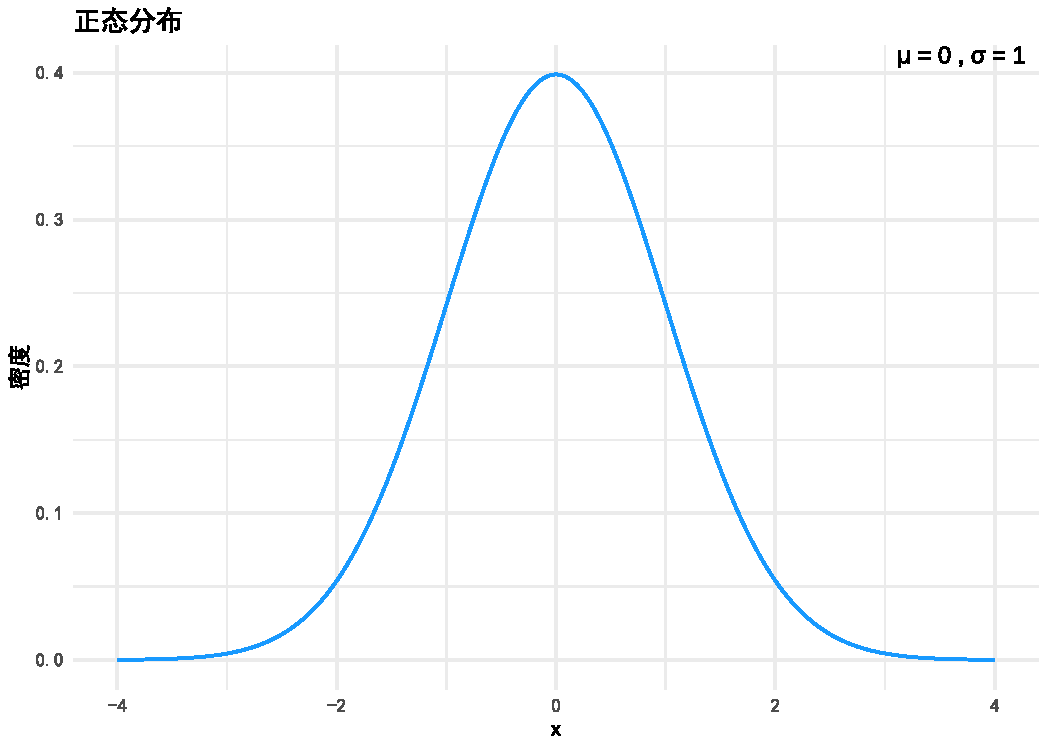
\includegraphics[width=\linewidth]{image/normal_distribution.pdf}}
		\subcaption{正态分布}
	\end{minipage}
	\hfill
	\begin{minipage}{0.48\textwidth}
		\centering
		\fbox{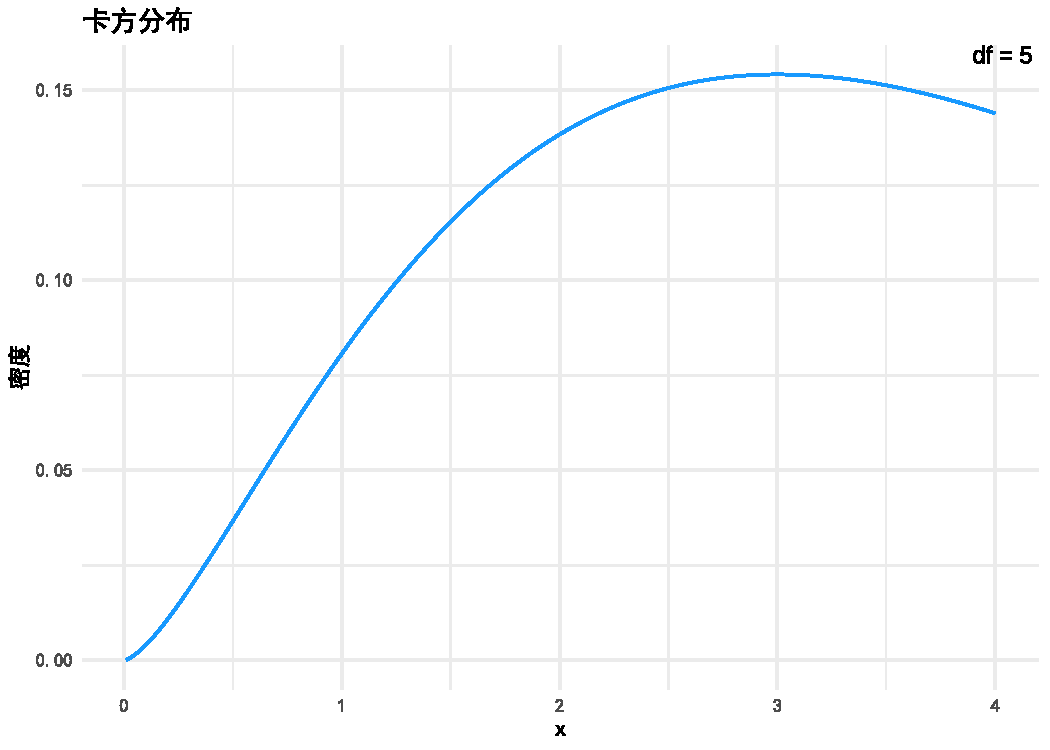
\includegraphics[width=\linewidth]{image/chi_squared_distribution.pdf}}
		\subcaption{卡方分布}
	\end{minipage}
	
	\vspace{1em}
	
	\begin{minipage}{0.48\textwidth}
		\centering
		\fbox{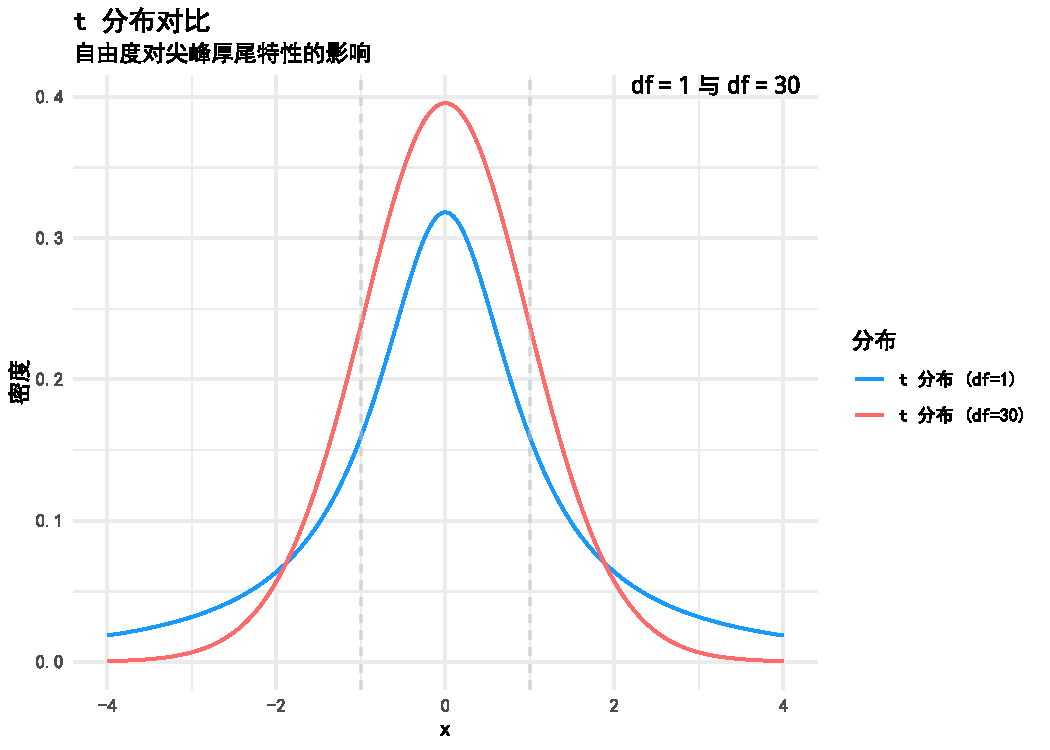
\includegraphics[width=\linewidth]{image/t_distribution_comparison.pdf}}
		\subcaption{$t$分布}
	\end{minipage}
	\hfill
	\begin{minipage}{0.48\textwidth}
		\centering
		\fbox{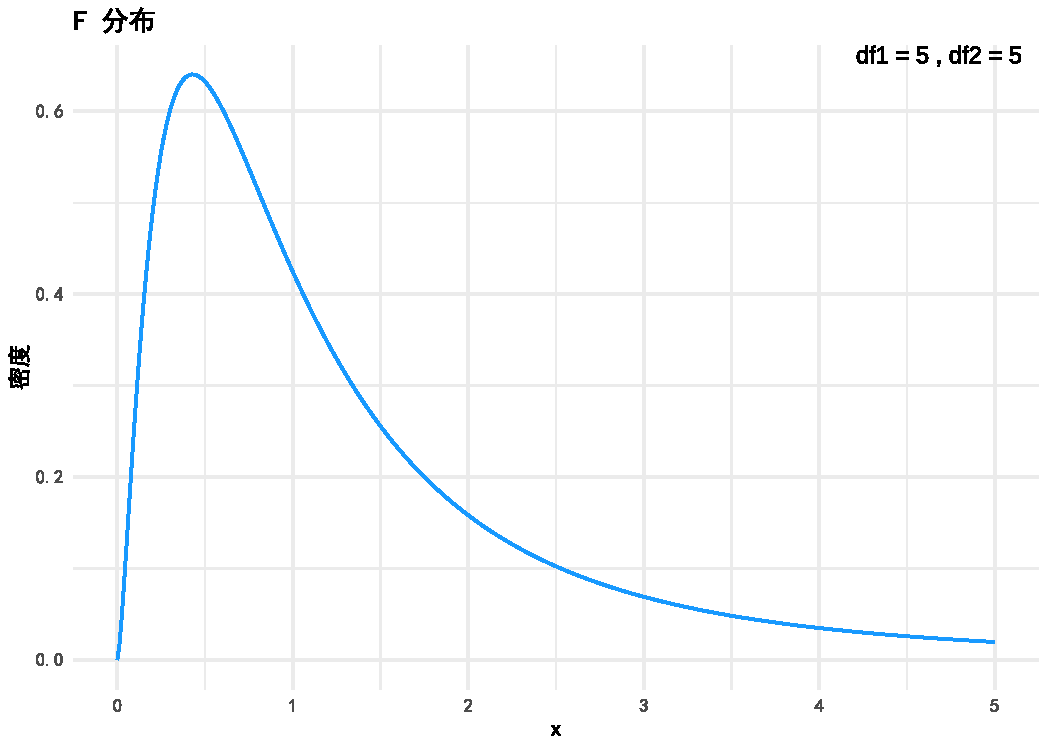
\includegraphics[width=\linewidth]{image/f_distribution.pdf}}
		\subcaption{$F$分布}
	\end{minipage}
	
	\caption{常见概率分布的比较}
	\label{fig:distributions}
\end{figure}

\subsection{统计推断的核心概念}

\paragraph*{总体与样本}
\begin{itemize}
	\item 总体(Population):研究对象的全体。
	\item 样本(Sample):从总体抽取的部分个体(容量$n$)。
	\item 理想样本:独立同分布(iid)随机样本。
\end{itemize}

\paragraph*{参数估计}
\begin{flushleft}
对于参数$\theta$,其估计量:
\end{flushleft}
\begin{equation}
	\hat{\theta} = \hat{\theta}(x_1,...,x_n) 
\end{equation}
\begin{itemize}
	\item 样本统计量(随机变量)。
	\item 估计值:给定样本时的具体取值。
\end{itemize}

\begin{flushleft}
常见估计量包括:
\end{flushleft}
\begin{align*}
	\text{样本均值} & : \bar{x} = \frac{1}{n}\sum x_i \\
	\text{样本中位数} & : \mathrm{median}(x_1,...,x_n) \\
	\text{极端值} & : \max/\min(x_1,...,x_n)
\end{align*}

\paragraph*{估计量的评价标准}
\begin{flushleft}
偏差的定义:
\end{flushleft}
\begin{equation}
	\mathrm{Bias}(\hat{\theta}) = E(\hat{\theta}) - \theta 
\end{equation}
当$E(\hat{\theta}) = \theta$时,称$\hat{\theta}$为无偏估计(unbias estimator),反之则为有偏估计(bias estimator)。

\paragraph*{均方误差(MSE)分解}
\begin{flushleft}
均方误差可以分解为方差与偏差平方之和:
\end{flushleft}
\begin{equation}
	\operatorname{MSE}(\hat{\theta})=\operatorname{Var}(\hat{\theta})+[\operatorname{Bias}(\hat{\theta})]^{2} 
\end{equation}

\begin{flushleft}
证明过程:
\end{flushleft}
\begin{equation}
	\begin{split}
		\operatorname{MSE}(\hat{\theta})&\equiv E\left[(\hat{\theta}-\theta)^{2}\right]\\
		&=E\left\{[\hat{\theta}-E(\hat{\theta})+E(\hat{\theta})-\theta]^{2}\right\} \\
		&=E\left[\hat{\theta}-E(\hat{\theta})\right]^{2}+2E\left\{[\hat{\theta}-E(\hat{\theta})][E(\hat{\theta})-\theta]\right\}+E[E(\hat{\theta})-\theta]^{2} \\
		&=\operatorname{Var}(\hat{\theta})+[\operatorname{Bias}(\hat{\theta})]^{2}
	\end{split}
\end{equation}

\begin{flushleft}
其中交叉项为0,因为:
\end{flushleft}
\begin{equation}
	E\{[\hat{\theta}-E(\hat{\theta})][E(\hat{\theta})-\theta]\}=[E(\hat{\theta})-\theta]\cdot 0=0 
\end{equation}

\paragraph*{偏差-方差权衡}
\begin{flushleft}
统计学的核心命题是均方误差可以分解为:
\end{flushleft}
\begin{equation}
	E\left[(\hat{\theta}-\theta)^{2}\right] = \underbrace{\mathrm{Bias}(\hat{\theta})^2}_{\text{近似误差}} + \underbrace{\mathrm{Var}(\hat{\theta})}_{\text{估计波动}} + \underbrace{\varepsilon}_{\text{随机误差}}
\end{equation}

\begin{flushleft}
极端案例对比:
\end{flushleft}
\begin{itemize}
	\item 无偏高方差估计量$\hat{\theta}$(如高阶多项式回归,易过拟合)
	\item 有偏低方差估计量$\tilde{\theta}$(如一次回归,可能欠拟合)
\end{itemize}

\begin{figure}[ht]
	\centering
	\fbox{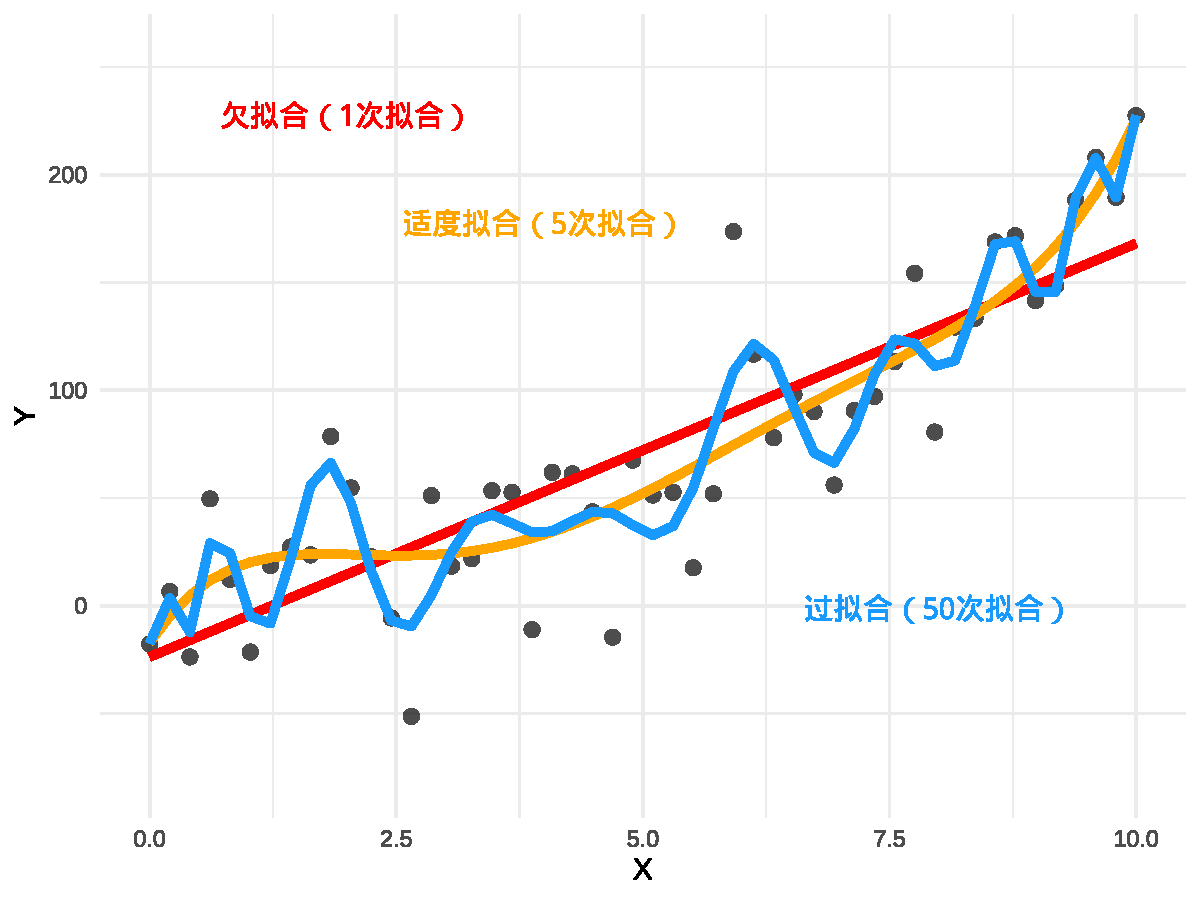
\includegraphics[width=0.5\linewidth]{image/fit_comparison}}
	\caption{拟合示例图}
\end{figure}

\section{社会科学中的统计推断}

\subsection{描述变量}

如何描述变量。这看似是一个简单的目标,但其内涵远比表面深刻。第二章讨论了如何建立研究问题,以及实证研究如何帮助我们理解世界,本章的前半部分回顾(预习)了基本的数学知识,此刻我们讨论变量描述。

实证研究问题本质上可归结为描述统计变量的密度分布——定量实证研究的核心就在于此。所有有趣的实证研究发现——无论是物理学、社会学、生物学、医学、经济学、政治学等领域——都有一条共同的主线。这条主线精巧地建立在概率基础之上,其形态表现为统计变量的密度分布,将整个宇宙中所有实证知识永恒地联系在一起。

为了理解数据,我们必须掌握如何观察并描述它们。这需要描述变量的类型及其分布形态。本节专注于单变量描述(后一节将讨论变量间的交互关系)。虽然单变量描述看似不如多变量分析有趣,但其重要性不容忽视。

在实证研究中,\textbf{变量}指对同一测量指标的一系列观测结果:如433名上海人的月收入、1999-2025年中国每年的企业并购数量、744名儿童的神经质心理评分、532朵花的颜色、《人民日报》上世纪某段时间内的头条新闻标题等。成功描述一个变量意味着能够清晰解释观测结果,而无需让他人查看所有原始数据。

\begin{flushleft}
描述变量的第一步是确定其类型。最常见的\textbf{变量类型}包括:
\end{flushleft}

\paragraph*{连续变量(Continuous Variables)}
连续变量可在一定范围内取任意值。例如上海人的月收入可以是12,000元,也可以是20,000元,或介于两者之间的任何值。这类变量没有``下一个最高''的概念,因为其变化是连续的。

\paragraph*{计数变量(Count Variables)}
计数变量记录事件发生的次数或物体的数量。例如中国每年的企业并购数量。计数变量不能为负值,也不能取分数值。当计数变量取值较多时,其性质接近连续变量,常被当作连续变量处理。

\paragraph*{有序变量(Ordinal Variables)}
有序变量的取值有``多''``少''之分,但缺乏精确的量化标准。例如神经质评分的``低''``中''``高''三个等级。虽然``高''高于``低'',但高多少并不明确。教育程度的``小学''``中学''``高中''``大学''也是有序变量——完成高中教育意味着比初中教育程度更高,但``高多少''无法精确量化。

\paragraph*{分类变量(Categorical Variables)}
分类变量记录观测对象所属的类别。例如花的颜色(白、橙、红)。这些类别没有高低之分,仅是不同类别。在社会科学研究中极为常见(如宗教信仰、种族、地理位置等)。\textbf{二元变量}是分类变量的特例,仅有两个取值(如``是/否'')。其优势在于便于处理实验效应(是否接受治疗),且多分类变量可转化为多个二元变量(如将政治面貌转化为``是否团员''``是否党员''等)。

\paragraph*{定性变量(Qualitative Variables)}
定性变量是非数值型、非分类的变量集合。如《人民日报》标题文本。这类变量通常包含大量难以概括的细节,常需转化为其他变量类型进行分析(如统计标题提及女性政治人物的次数,或使用AI模型进行特征评分)。

\begin{flushleft}
确定变量类型后,下一步是考察其\textbf{分布}——描述变量各取值出现概率的特征。
\end{flushleft}

\paragraph*{分布描述}
对于分类或有序变量,可通过给出各类别/取值的百分比来描述分布。完整分布可通过频率表或条形图展示。

\begin{table}[h]
	\centering
	\renewcommand{\arraystretch}{1.5}
	\caption{美国高校学位类型分布}
	\begin{tabularx}{1\linewidth}{>{\raggedright\arraybackslash}Xcc}
		\toprule
		授予的主要学位类型 & 数量(N) & 百分比(\%) \\
		\midrule
		两年制以下学位 & 3495 & 47 \\
		两年制学位 & 1647 & 22 \\
		四年制及以上学位 & 2282 & 31 \\
		总计 & 7424 & 100 \\
		\bottomrule
	\end{tabularx}
\end{table}

\begin{figure}[ht]
	\centering
	\fbox{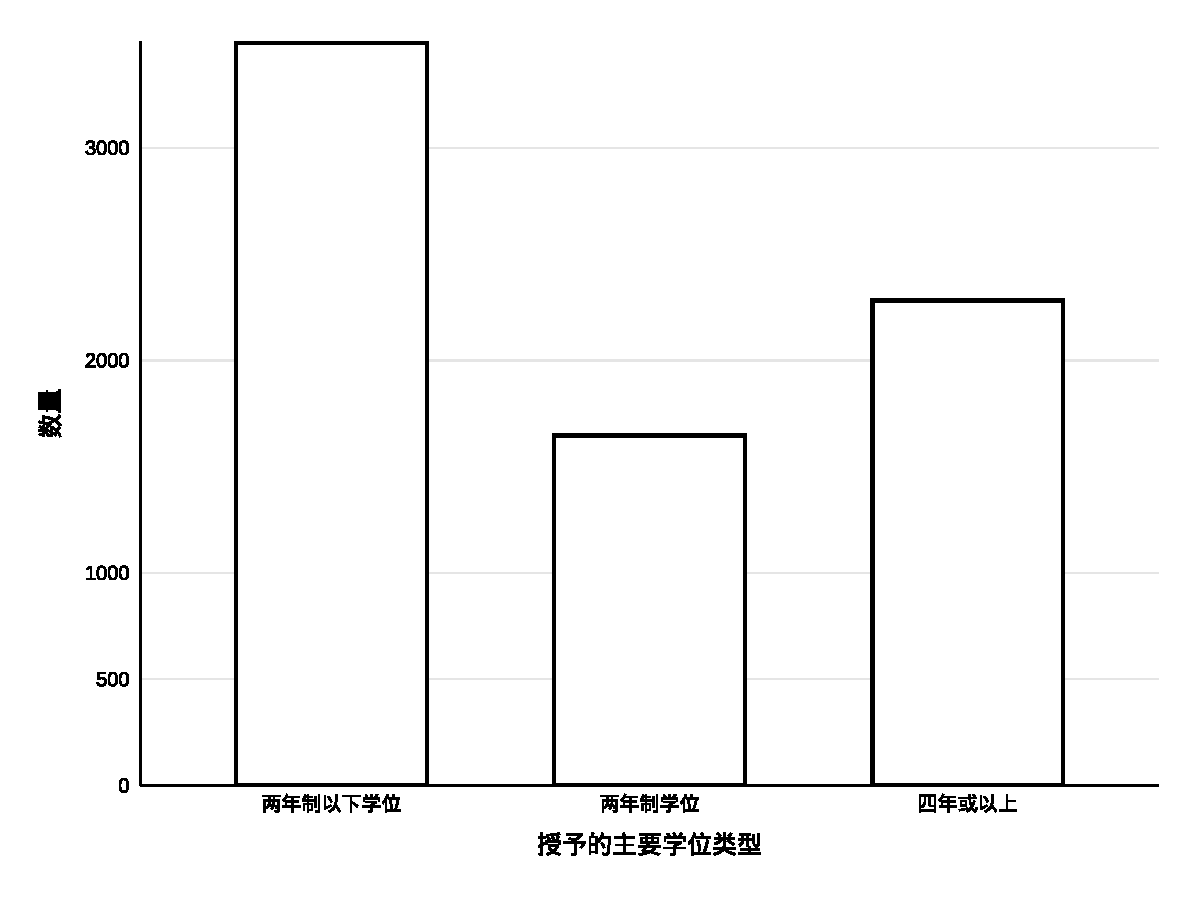
\includegraphics[width=0.5\textwidth]{image/earnings_distribution.pdf}}
	\caption{美国高校毕业生平均收入分布图}
	\label{fig:earnings}
\end{figure}


连续变量的分布描述更为复杂。由于观测值重复概率低,需采用\textbf{直方图}(将数据范围划分为区间并显示各区间的观测比例)或\textbf{密度图}(显示当直方图区间无限变窄时的极限形态)。密度曲线下面积代表概率,如图\ref{fig:earnings}所示,16\%的观测值位于40,000至50,000美元区间。

当完整分布信息量过大时(尤其对连续变量),需用少量数字概括分布特征。最经典的例子是\textbf{均值}——将所有观测值相加后除以观测数。均值代表数据的中心趋势,试图生成一个代表性数值。

\paragraph*{百分位数(Percentiles)}
\textbf{X百分位数}指X\%的观测值小于该值的点。例如身高数据的第5百分位数为5英尺4英寸。中位数(第50百分位数)是另一种中心趋势度量,代表典型观测值(对偏斜数据更稳健)。最小值和最大值(第0和100百分位数)显示变量的取值范围,其差值称为\textbf{极差}。

\paragraph*{变异度量}
变量间变异程度不同(如子女人数变异较大,而眼睛数量变异较小)。\textbf{方差}是基于均值的变异度量:
\begin{enumerate}
	\item 计算均值
	\item 各观测值减均值(得离均差)
	\item 离均差平方
	\item 求平方和
	\item 除以观测数减1(得样本方差)
\end{enumerate}

为消除平方单位影响,常取方差的平方根得\textbf{标准差}(恢复原始单位)。标准差有助于评估观测值的相对位置(如收入38,000美元者比均值高37.6\%个标准差)。

\paragraph*{四分位距(IQR)}是第75与25百分位数之差,覆盖样本中50\%最接近中位数的观测值,对极端值不敏感。

\paragraph*{偏度(Skew)}
偏度描述分布向一侧倾斜的程度。例如年收入分布有长右尾(少数极高收入者),称为\textbf{右偏}。左偏分布则有长左尾。对称分布则两侧尾部相近。

处理偏斜数据的常用方法是对数转换(使数据更接近正态分布)。自然对数转换的优势在于系数解释直观(对数增加0.01约对应原始变量1\%的增长)。

统计学严格区分\textbf{真相}(理论分布)与\textbf{数据}(观测分布)。我们真正关心的是理论分布(生成数据的分布),而非样本统计量。随着样本量增加,观测分布会趋近理论分布。

\paragraph*{常见理论分布}
\begin{itemize}
	\item \textbf{正态分布}:对称分布(如身高、智商)。即使严格意义上不适用(如身高不能为负),但当近似良好时仍被广泛采用。
	\item \textbf{对数正态分布}:取对数后呈正态分布的右偏分布(如收入、财富、公司规模等)。其优势在于可通过对数转换消除偏度。
\end{itemize}

\paragraph*{假设检验中的 \(H_0\) 和 \(H_1\)}

在统计推断中,假设检验是判断样本数据是否支持某一假设的核心方法。我们通常定义:
\[
\begin{cases}
H_0: \text{原假设(Null Hypothesis),一般表示无效假设或无差异}\\
H_1: \text{备择假设(Alternative Hypothesis),表示研究者关心的效应存在或差异存在}
\end{cases}
\]
检验的目标是基于样本数据决定是否拒绝 \(H_0\),从而间接支持 \(H_1\)。

\paragraph*{第一类错误与第二类错误}

由于样本具有随机性,假设检验不可避免地存在两种错误:

\begin{itemize}
	\item \textbf{第一类错误(``弃真''错误):} 当 \(H_0\) 为真时,错误地拒绝了 \(H_0\)。犯此错误的概率称为显著性水平 \(\alpha\)。
	\item \textbf{第二类错误(``取伪''错误):} 当 \(H_1\) 为真时,错误地未拒绝 \(H_0\)(即接受了错误的原假设)。犯此错误的概率用 \(\beta\) 表示。
\end{itemize}

显著性水平 \(\alpha\) 通常事先设定(如 0.05),用于控制第一类错误概率的上限。第二类错误概率 \(\beta\) 反映检验的``检验力''(Power),即正确拒绝错误的原假设 \(H_0\) 的能力,其值为 \(1-\beta\)(例如检验力为 0.95 表示有 95\% 的概率能够正确拒绝无效的原假设。)。

回顾第一章中波普尔的观点——科学中没有不能被质疑的陈述。科学普遍理论的基本命题必须是可证伪的,即应当能够通过实证加以检验和潜在的反驳。

在科学实践中,我们更倾向于积极检验理论,力图通过证据去反驳,而非轻易接受某个理论。因此,统计检验通常强调控制第一类错误(显著性水平 \(\alpha\)),以避免盲目拒绝真实理论。同时,在科学探索中,第一类错误的风险通常被视为较为可控的代价,而错误接受错误理论(第二类错误)可能更严重地阻碍科学进步。

因此,标准的统计推断做法是:只要样本数据提供的证据足够强(即 \(p\) 值小于预设的显著性水平 \(\alpha\)),就拒绝原假设 \(H_0\)。但需要明确的是,拒绝 \(H_0\) 并不意味着备择假设 \(H_1\) 必然为真,仅表明数据与 \(H_0\) 不符,支持 \(H_1\) 的可能性较大。统计推断本质上是概率性的,而非绝对确定。

\paragraph*{从数据推断理论分布}
我们可通过假设检验评估理论分布的可能性:
\begin{enumerate}
	\item 选择理论分布的某个特征(如均值$\mu$)
	\item 基于理论分布性质和样本量,确定该特征在随机样本中的抽样分布
	\item 计算观测数据的对应特征
	\item 评估观测结果在理论分布中的出现概率
	\item 若概率极低,则拒绝原理论分布假设
\end{enumerate}
	
\vspace{0.8em} % 手动调整间距

\begin{example}
	篮球运动员得分数据样本中有100个数据,得分均值为102,标准差为30($n=100$,$\bar{x}=102$,$s=30$),假设理论均值$\mu=90$成立吗?
	
\begin{flushleft}	
1. 抽样分布的推导
\end{flushleft}
根据中心极限定理(Central Limit Theorem, CLT),当样本大小 \(n\) 足够大时(一般 \(n \geq 30\)),样本均值的抽样分布近似正态分布:
\begin{itemize}
	\item 分布的均值等于总体均值(在 \(H_0\) 下,\(\mu = 90\))。
	\item 分布的标准差(称为标准误差,\(\sigma_{\bar{x}}\)) 由公式 \(\sigma_{\bar{x}} = \frac{s}{\sqrt{n}}\) 计算。
\end{itemize}

\begin{flushleft}
给定数据:n = 100, \quad s = 30
\end{flushleft}

\begin{flushleft}
计算标准误差:
\end{flushleft}
\begin{equation}
\sigma_{\bar{x}} = \frac{s}{\sqrt{n}} = \frac{30}{\sqrt{100}} = \frac{30}{10} = 3
\end{equation}
因此,在 \(H_0\) 下,样本均值的抽样分布是正态分布 \(N(90, 3)\)(即均值为 90,标准差为 3)。这可以写为:
\begin{equation}
\bar{X} \sim N(\mu, \sigma_{\bar{x}}^2) = N(90, 3^2) = N(90, 9)
\end{equation}
(注:\(N(\mu, \sigma^2)\) 表示正态分布,其中第二个参数是方差;标准差为 \(\sigma = 3\),方差为 \(\sigma^2 = 9\)。在推断中,通常直接使用标准差。)

\begin{flushleft}	
2. 检验统计量(z-分数)的计算
\end{flushleft}
观测样本均值 \(\bar{x} = 102\)。我们计算其与假设均值 \(\mu = 90\) 的差异,并以标准误差为单位标准化:
\begin{equation}
z = \frac{\bar{x} - \mu}{\sigma_{\bar{x}}} = \frac{102 - 90}{3} = \frac{12}{3} = 4
\end{equation}
z-分数为 4,表示观测均值 \(\bar{x} = 102\) 与假设均值 \(\mu = 90\) 相差 4 个标准误差(即 4 个标准差单位)。这反映了在 \(H_0\) 下,观测值的相对位置。

\begin{flushleft}	
3. p-值的解释
\end{flushleft}
p-值是在 \(H_0\) 成立时,观测到与样本均值一样极端或更极端结果的概率。这是一个双尾检验(因为 \(H_1: \mu \neq 90\)),因此:
\begin{equation}
\text{p-value} = P(|\bar{X}| \geq |\bar{x}| \mid H_0) \approx P(|Z| \geq 4) \quad \text{(其中 } Z \sim N(0,1)\text{)}
\end{equation}
在标准正态分布下:
\begin{itemize}
	\item \(P(Z \geq 4) \approx 0.00003167\)(右尾概率)。
	\item 双尾 p-值 \(\approx 2 \times 0.00003167 = 0.00006334\)。
\end{itemize}
因此,p-值远小于 0.0001(即 \(p < 0.0001\))。这表明,如果 \(H_0\) 为真(\(\mu = 90\)),观测到样本均值 \(\bar{x} = 102\)(或更极端)的概率极低(小于万分之一),属于统计学上的极端事件。

\begin{flushleft}
4. 结论
\end{flushleft}
给定显著性水平 \(\alpha = 0.05\)(常用阈值):
\begin{equation}
\text{p-value} < 0.0001 < 0.05 = \alpha
\end{equation}
因此,我们有非常强的证据拒绝原假设 \(H_0: \mu = 90\)。结论是:篮球运动员的平均得分不太可能是 90,更可能高于此值。

\end{example}

\subsection{描述关系}

对于大多数研究问题,我们不仅对单个变量的分布感兴趣,更关注数据中两个或多个变量之间的关系。两个变量之间存在关系意味着什么?这种关系显示了了解一个变量能为我们提供关于另一个变量的信息。

例如儿童的身高与年龄。通常,孩子年龄越大,身高越高。因此知道一个孩子13岁而另一个6岁,就能较好地猜测谁更高。我们可以称身高与年龄的关系为``正相关''——一个变量的较高值往往对应另一个变量的较高值(年龄越大身高越高)。也存在``负相关''关系(年龄越大哭闹越少),以及``零相关''关系(儿童年龄与居住可能性无关)。其他关系可能时正时负,或初期强正相关后期弱正相关。若变量是分类变量,则不存在``高低''之分,只有``差异''(大孩子更可能骑自行车上学)。

\paragraph*{条件分布}

上一章讨论的是变量的无条件分布(也称边缘分布)。条件分布则是指给定另一个变量特定值时,某个变量的分布。

以条件概率为例:随机一个人是女性的概率约50\%,但名叫\textbf{翠花}的人是女性的概率远高于50\%。我们称之为``在名为翠花的条件下是女性的概率''。条件分布同理,不过是从单一概率扩展到整个分布的变化。

图\ref{fig:vitaminE}展示了服用维生素E剂量的分布,按是否进行剧烈运动分组。可见运动者与非运动者的分布存在差异——运动者服用剂量更大。这种分布差异表明维生素E摄入与运动存在关联。

\begin{figure}[ht]
	\centering
	\fbox{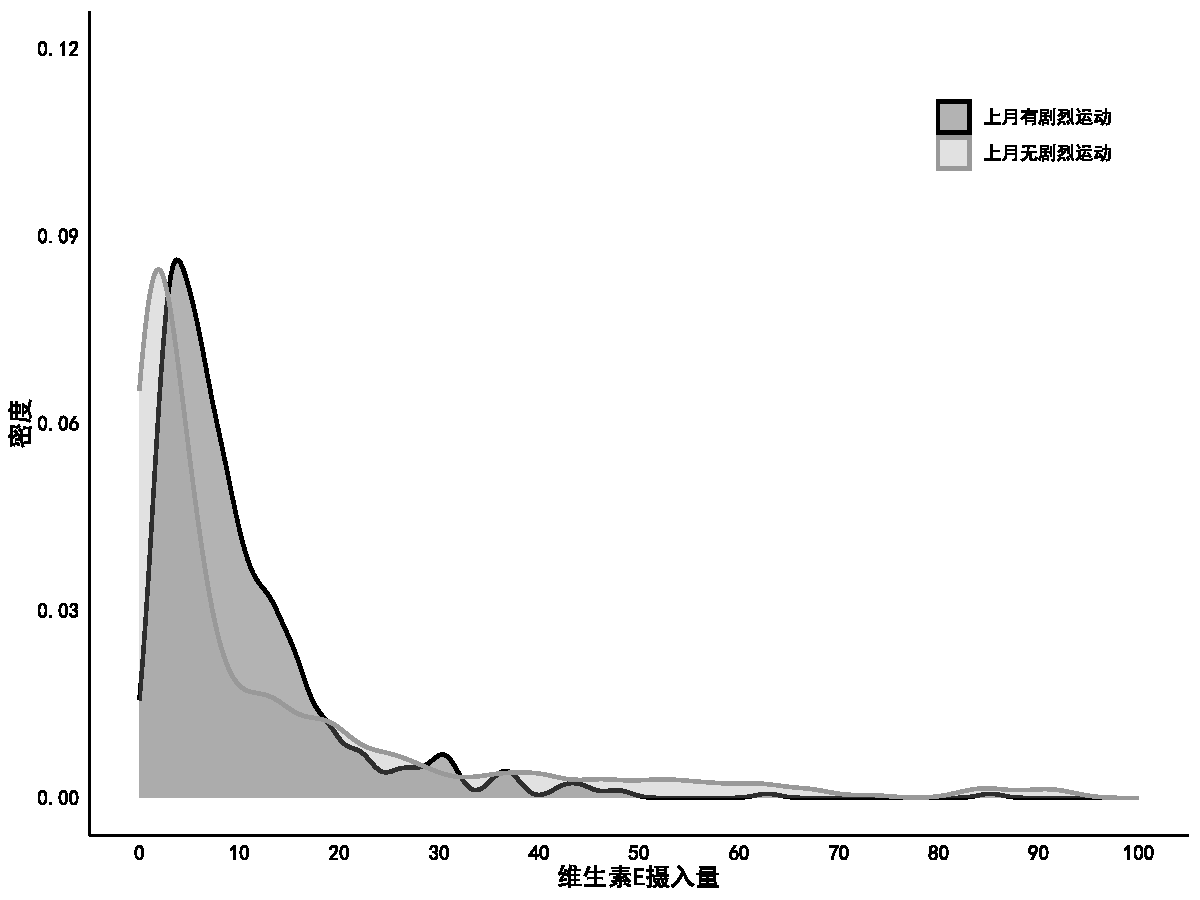
\includegraphics[width=0.5\textwidth]{image/vitaminE_density.pdf}}
	\caption{上月运动情况对维生素E摄入量的影响}
	\label{fig:vitaminE}
\end{figure}

该概念同样适用于分类变量。图\ref{fig:vitaminEbarchart}显示:不吸烟人群服用维生素E的比例明显高于吸烟人群,这与Oster关于健康意识驱动行为的假设一致。

\begin{figure}[ht]
	\centering
	\fbox{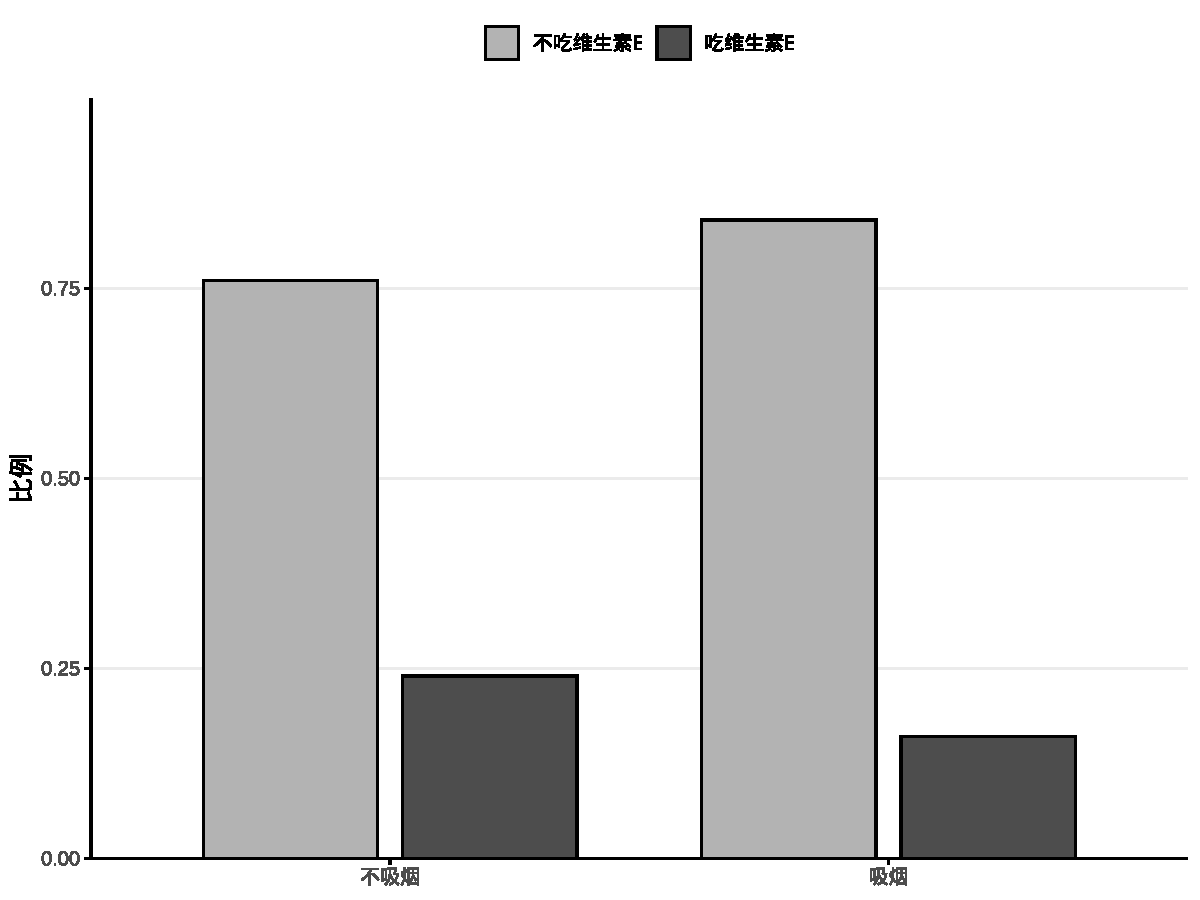
\includegraphics[width=0.5\textwidth]{image/vitaminE_barchart.pdf}}
	\caption{是否吸烟与是否服用维生素E的关系}
	\label{fig:vitaminEbarchart}
\end{figure}

\paragraph*{条件均值}

掌握条件分布概念后,我们可计算该分布的任何特征。本章重点讨论条件均值——给定变量$X$的特定值,变量$Y$的期望均值。

对于离散变量,计算简单:只需取该值所有观测的均值。图\ref{fig:VitaminE_by_BMI}显示维生素E服用比例随时间阶段(推荐前/中/后)的变化:推荐期间呈现正相关,推荐取消后转为负相关。

\begin{figure}[ht]
	\centering
	\fbox{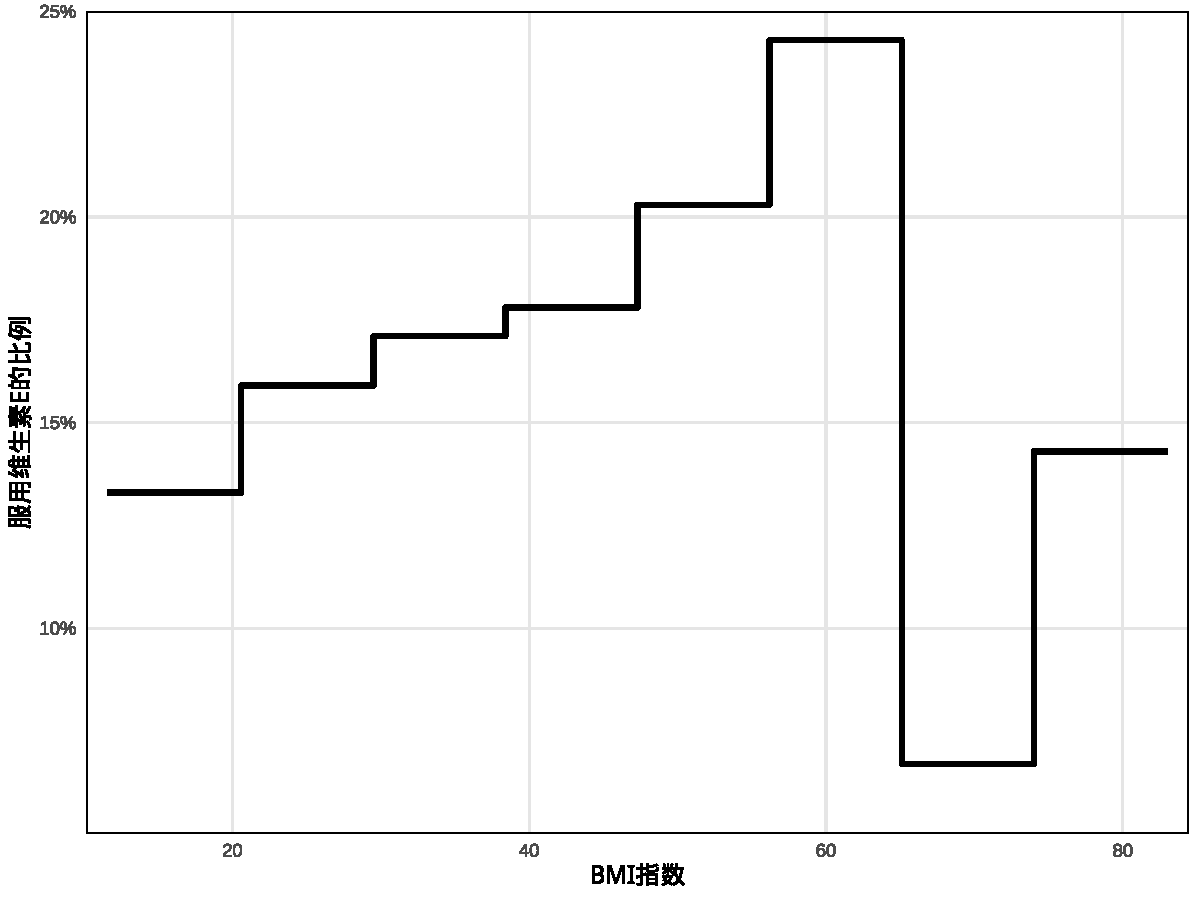
\includegraphics[width=0.5\textwidth]{image/VitaminE_by_BMI.pdf}}
	\caption{按体重指数值范围分列的服用维生素E的比例}
	\label{fig:VitaminE_by_BMI}
\end{figure}

连续变量则更复杂。解决方法有两种:
\begin{enumerate}
	\item 将连续变量划分为若干区间(分箱),计算各区间内均值
	\item 使用局部均值或LOESS曲线(局部加权散点平滑)进行平滑处理
\end{enumerate}

图\ref{fig:LOESS_Curve}的LOESS曲线清晰显示:BMI越高,维生素E服用率越高,初期关系强烈后期趋于平缓。这种方法通过移动窗口计算局部均值,避免分箱法的任意性缺陷。

\begin{figure}[ht]
	\centering
	\fbox{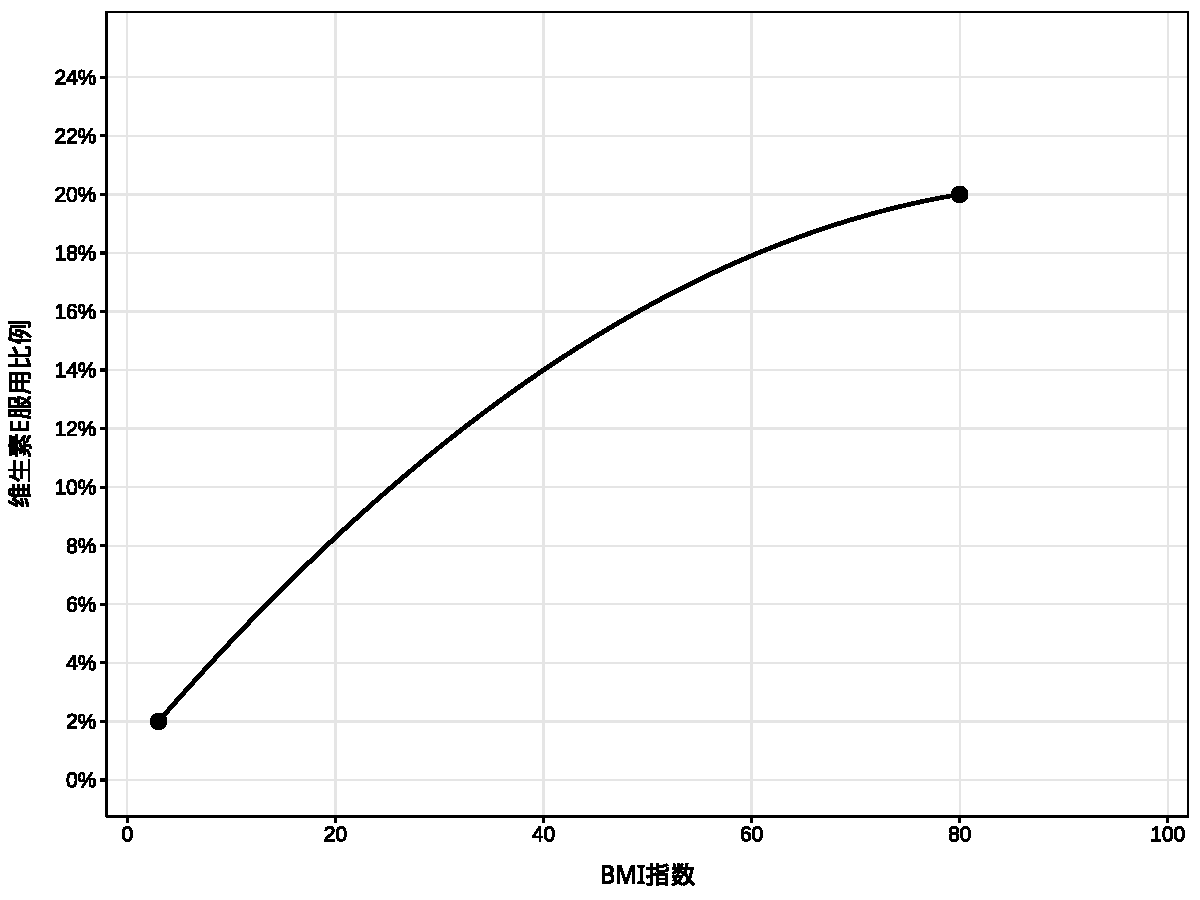
\includegraphics[width=0.5\textwidth]{image/LOESS_Curve.pdf}}
	\caption{按体重指数(BMI)划分的服用维生素 E 的比例(LOESS)曲线}
	\label{fig:LOESS_Curve}
\end{figure}

\paragraph*{回归分析}

另一种方法是假设变量间存在某种数学关系(通常是直线),即回归分析。图\ref{fig:VitaminE_BMI_linear}用直线拟合维生素E与BMI的关系,斜率0.002表示BMI每增加1单位,服用概率上升0.2个百分点。

\begin{figure}[ht]
	\centering
	\fbox{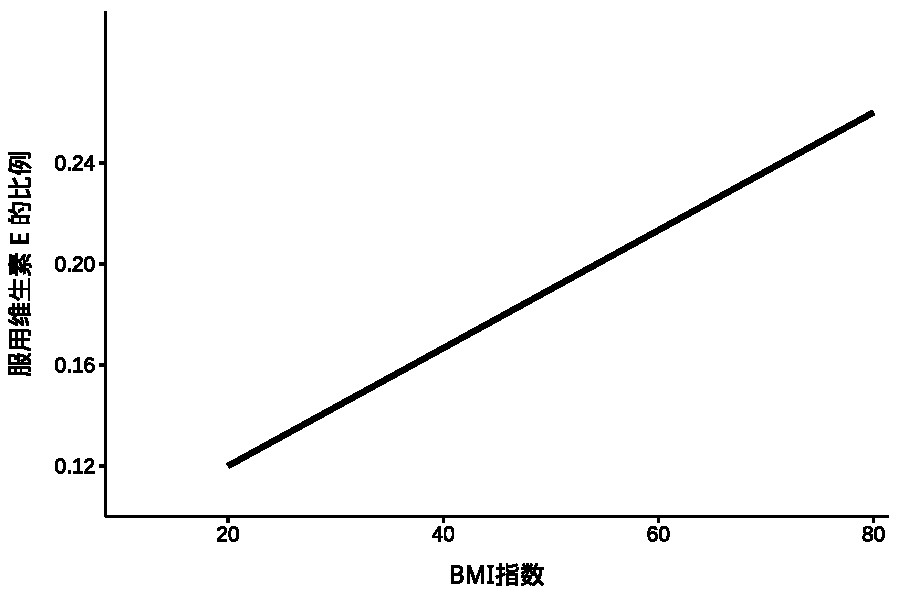
\includegraphics[width=0.5\textwidth]{image/VitaminE_BMI_linear.pdf}}
	\caption{用拟合直线表示按体重指数计算的服用维生素E的比例}
	\label{fig:VitaminE_BMI_linear}
\end{figure}

普通最小二乘法(OLS)是最常用的直线拟合方法,通过最小化残差平方和确定最佳直线。其斜率计算公式为协方差除以$X$的方差,直观反映了``$X$的变化中有多少与$Y$协同变化''。

当直线拟合不足时,可采用:
\begin{itemize}
	\item 多项式回归(如二次曲线)
	\item 非线性转换(如对数、概率单位转换)
\end{itemize}

\paragraph*{条件均值(``控制变量'')}

通过回归残差,我们可以剥离已解释部分,专注于未被解释的变异。将这个方法应用于双变量,就能实现``控制变量''——消除$Z$对$X$和$Y$的影响后,分析二者的纯净关系。

多元回归是最高效的实现方式,在仅考虑BMI时,我们估计:
\begin{equation}
	\text{VitaminE} = .110 + .002 \times \text{BMI}
\end{equation}

现在加入BMI、性别和年龄后,得到:
\begin{equation}
	\text{VitaminE} = -.006 + .001 \times \text{BMI} + .002 \times \text{Age} + .016 \times \text{Female}
\end{equation}

在控制年龄和性别后,BMI的效应从0.002降至0.001,说明原关系部分由这些变量解释。同时,年龄每增加1岁服用概率提高0.2个百分点,女性比男性高1.6个百分点。

这种方法在数学上对应Frisch-Waugh-Lovell定理:通过回归残差间的回归,等效于直接进行多元回归。这让我们能清晰分离不同变量的独立影响。

\newpage
\thispagestyle{empty}
\begin{thebibliography}{99}
	\bibitem{1}
	陈强,《计量经济学及Stata应用(第2版)》,高等教育出版社
	
	\bibitem{2}
	Nick Huntington-Klein,《The Effect》,CRC Press
	
\end{thebibliography}

\chapter{因果推断的源流原理}
\section{计量与因果}
\subsection{计量经济学的历史与发展}

1930年代,以计量经济学会成立为标志,经济学中的实证方法成为一个独立学科出现。

在计量经济学内部又可以分为两大部门,1950-60年代,宏观计量大发展,Klein、Stone等学者推动了以结构计量或模型为基础的计量经济学(Model-based Econometrics)。研究者首先先验地定好各变量之间的函数关系,再代入当下的宏观变量进行验证和改进,由于石油危机的出现,路径依赖下的结构计量遭遇滑铁卢,断点的产生使得精巧的模型与复杂的现实间的宏观难以逾越,更多人选择抛弃结构而转向设计。

潜在结果框架(Potential Outcome Framework)的发展可以分为以下几个阶段:

\begin{enumerate}
	\item 生物学实验设计的萌芽:早期应用可追溯至18世纪林德医生(James Lind)的坏血病对照实验。他通过将船员分组并给予不同治疗方案(如柑橘类水果),首次以实验设计验证了因果效应。这一案例虽未形式化潜在结果概念,但体现了“反事实比较”的核心思想。
	\item 休厄尔·赖特、豚鼠和路径图:20世纪20年代,遗传学家休厄尔·赖特(Sewall Wright)通过研究豚鼠的遗传学,发展出了路径分析(Path Analysis)方法。他用图表来表示变量之间的因果关系,并用路径系数来量化这些关系。这一工作为后续因果推断的发展提供了重要的理论基础。,这一理论后来成为结构方程模型(Structural Equation Modeling, SEM)和结构因果模型(Structural Causal Modeling, SCM)的基础。
	\item 统计学的理论奠基:20世纪20-30年代,Neyman在随机化试验中首次提出潜在结果的数学表述,但直到1990年其论文英译后才广为人知。\href{https://doi.org/10.1037/h0037350}{Rubin(1974)}将潜在结果扩展至观察性数据,正式建立Rubin因果模型,解决了非随机实验中的因果识别问题。
\end{enumerate}

即使在结构计量之中,潜在结果的概念也已经有所体现。挪威经济学家 Trygve Haavelmo 在1943年研究联立方程模型(SEMs)时,探讨了供求模型中的识别问题(identification)。他区分了供求函数中的“任何想象的价格 π”和“实际观察到的均衡价格 p”,并将实际价格下的供求量视为特定条件下的实现结果(\href{https://doi.org/10.2307/1905714}{Haavelmo, 1943})。这一区分隐含了潜在结果的思想。因此,Haavelmo 被视为计量经济学概率论基础的奠基人之一(\href{https://doi.org/10.1257/jel.47.1.5}{Imbens \& Wooldridge, 2009};\href{https://doi.org/10.1214/08-AOAS187}{Rubin, 2008})。

当然,计量经济学后续的发展并没有沿着这一方向继续深入。到了20世纪中叶,主流方法转向直接对观测结果建模,将潜在结果与分配机制混杂在一起,导致以下问题:

\begin{enumerate}
	\item 因果效应识别变得难以理解;
	\item 需要引入越来越多的强假设;
	\item 模型对设定误设(misspecification)非常敏感。
\end{enumerate}

\href{https://www.jstor.org/stable/1803924}{Leamer (1983)}指出:"计量经济学的艺术就是,研究者在计算机终端中拟合许多(甚至上千个)统计模型,从中选择一个或几个符合作者预期的估计结果在论文中进行报告。"他发现"我们正处于一种令人沮丧和不科学的境地。没有人将数据分析看作严肃的事情,或者更准确地,没有人把别人的数据分析当回事。"他提议将计量经济学中的"谎言和欺骗"剔除出来,并提出了"敏感性分析"(sensitivity analysis)作为解决方案。

\href{https://www.jstor.org/stable/1806062}{LaLonde (1986)} 利用美国1970年代进行的一项就业培训的随机化实验数据,考察传统计量经济学方法是否能够模拟随机化实验的结果。他以随机化实验作为基准(benchmark),利用观测数据作为控制组,运用回归、固定效应、Heckman选择模型等计量经济学常用方法估计了培训对收入的影响,发现这些方法都无法复制随机化实验的结果。这一研究得出了在观察研究中计量经济学方法无法可信地估计因果效应的悲观结论。

\href{https://doi.org/10.1080/01621459.1999.10473858}{Dehejia和Wahba (1999)} 利用倾向指数匹配方法重新考察了\href{https://www.jstor.org/stable/1806062}{LaLonde (1986)} 探讨的问题。他们发现,尽管LaLonde尽量通过手工方式使两组个体相似,但构造的控制组个体与实验中的干预组个体仍然具有较大的特征差异。通过倾向指数匹配方法,他们获得了与干预组更为相似的控制组,发现估计的因果效应与随机化实验的结果非常相似。

1990年代左右,\href{https://doi.org/10.1177/001979399004300205}{Card (1990)}、\href{https://www.jstor.org/stable/2006669}{Angrist (1990)}、\href{https://doi.org/10.3386/w4509}{Card和Krueger (1994)}、\href{https://doi.org/10.1080/01621459.1996.10476902}{Angrist、Imbens和Rubin (1996)}、\href{https://doi.org/10.1162/003355399556061}{Angrist和Lavy (1999)}、\href{https://doi.org/10.3982/ECTA11293}{Abadie和Imbens (2003)}、\href{https://doi.org/10.1198/jasa.2009.ap08746}{(Abadie、Diamond和Hainmueller 2010)}的一系列研究,将经济学实证研究重新回到科学发展的开端,使内部有效性更好,实证结果更可信,从而引发了一场经济学经验研究的"可信性革命"(Angrist和Pischke,2010)或"自然实验革命"\href{https://doi.org/10.1037/a0018538}{(Imbens,2010)}。

2019年,Abhijit Banerjee、Esther Duflo和Michael Kremer因利用随机化实验研究全球减贫问题而获得诺贝尔经济学奖,如教育、医疗与农业帮扶等对印度等地的赤贫人口的帮助作用;2021年,David Card因利用两地政策变动不一的“自然实验”,比较最低工资法颁布对就业的影响、Joshua Angrist和Guido Imbens因对因果推断方法论贡献而获得诺贝尔经济学奖;2024年,Daron Acemoglu、Simon Johnson和James A. Robinson因其利用殖民地死亡率这一工具变量研究对制度如何形成并影响繁荣的研究而获奖。这些发展标志着基于设计的计量范式(Design-based Econometrics)的兴起。

当下的经济学经验研究正在经历了一场深刻的“可信性革命”,这场革命的核心在于从根本上改变了研究者进行实证分析的方法论取向。这场革命主要包含两个关键内容:首先是更加注重因果推断而非简单的相关性分析,其次是特别强调研究设计在实证分析中的核心地位。

具体而言,可信性革命引入了潜在结果框架(Potential Outcomes Framework),为因果关系的定义和识别提供了严谨的理论基础。在这一框架下,研究者致力于通过巧妙的研究设计,使观测性研究能够尽可能模拟随机化实验的理想条件。这种转变使得经济学实证研究能够获得更接近真实因果效应的估计结果。

“设计”是这场革命的核心所在。传统的估计方法如普通最小二乘法(OLS)、最大似然估计(MLE)和广义矩估计(GMM)本质上都只是统计工具,它们本身并不能保证因果关系的识别。相比之下,匹配方法(Matching)、工具变量法(IV)、双重差分法(DID)和合成控制法(Synthetic Control)等新兴方法则更加注重研究设计环节。这些方法通过精心设计的研究方案,模拟随机化实验的条件,在完成设计后,即使是简单的OLS回归也能得到可信的因果效应估计。

这种以设计为导向的研究范式主要致力于解决实证分析中的两个关键问题:
\begin{enumerate}
	\item 消除混杂因素导致的偏差(Confounding Bias)
	\item 样本选择偏差(Selection Bias)。
\end{enumerate}

通过这种转变,经济学实证研究的内部效度得到了显著提升,研究结果的政策指导意义也大大增强。正如Angrist和Pischke(2010)所强调的,这场革命使得经济学实证研究重新回归科学方法的本源,为学科发展注入了新的活力。

至此,计量经济学家重新认识到潜在结果框架的重要性,并推动了一场被称为“可信性革命”的学术运动。这场革命强调因果推断的严谨性和可验证性,代表人物包括:Guido Imbens(斯坦福大学);Joshua Angrist(麻省理工学院);Alberto Abadie(MIT);David Card(加州大学伯克利分校)。他们倡导以实验设计的思维方式来处理因果推断问题,被广泛称为计量经济学的“实验学派”。

\subsection{因果关系与求异法}

相关不等于因果,这成了大众普遍的认知,然而在实验设计为导向的现代计量当中,由于事先的分析,相关终于是为因果开辟了道路,为了更好理解实验设计,我们有必要首先习得因果关系如何识别。

二战期间,美国空军希望研究应优先在轰炸机的哪些部位加装防护装甲,以提高飞机的返航率。为此,他们收集了所有成功返航的飞机,并详细记录了这些飞机上遭受弹孔的位置。数据显示,机翼、机尾和机身等部位的弹孔较多,而发动机部位则几乎没有弹孔。根据这一观察,不少人认为应当在弹孔密集的区域加装装甲。

然而,统计学家亚伯拉罕·瓦尔德(Abraham Wald)提出了完全相反的建议。他指出,数据仅来自成功返航的飞机,而那些被击中发动机却未能返航的飞机并未被纳入观察范围。因此,发动机弹孔少恰恰意味着这些部位一旦被击中,飞机便难以生还。因此,应当将防护重点放在看似“未中弹”的发动机部位。

这个案例清晰地揭示了一个重要问题:我们所观察到的数据并不总是完整或无偏的。在社会科学研究中,这种“样本选择偏差”(sample selection bias)极为常见。我们往往只能接触到某种“幸存者样本”,而无法观察到那些由于某种机制而未能进入样本的个体。因而,仅凭已有数据得出的统计关联,未必反映真实的因果结构。

在社会科学研究中,类似瓦尔德的“反向思考”极为重要。许多情况下,我们所拥有的数据并不足以直接支持一个可靠的因果推断。我们需要意识到,哪些变量能够进入我们的分析视野,本身就可能受到制度、选择机制或测量限制的影响。

另一个典型案例是家长择校问题。许多家长简单地将学校升学率等同于教育质量。例如,国际学校学生普遍表现优异,但这可能源于其学生家庭背景的优势。这里,家庭背景作为第三变量,同时影响了学校选择和学业表现。这一现象称为“虚假相关”(spurious correlation),其根源在于存在一个共同影响因变量与自变量的“第三变量”(confounder)。若未能识别并控制这些混淆变量,我们所进行的因果推断将缺乏有效性,甚至可能产生误导。

为应对这一挑战,科学研究提出了“控制实验”的基本逻辑。其核心思想是:通过人为操纵某一变量(自变量),并在其他条件保持一致的情况下,观察结果变量(因变量)的变化,从而识别是否存在因果效应。

大航海时代是人类历史上地理大发现的开端,也是全球化进程的一个关键阶段。在这一英雄辈出的时代背景下,坏血病成为横亘于航海探索之路上的巨大障碍。据历史统计,在1500年至1800年期间,约有超过200万航海人员死于坏血病,平均每年约6700人。因此,坏血病可被视为大航海时代的一种“时代性疾病”。

一个典型的例证出现在1740年英国海军的一次环球航行中。在此次航行中,舰队起航后的十个月内,1900名船员中有多达1400人因坏血病死亡。更具启发性的是,比较同期不同国家海员的病亡数据发现,英国海员的坏血病死亡率明显高于法国与西班牙海员,这引发了关于疾病分布与饮食文化之间关系的深层次讨论。

值得注意的是,与西方国家的情况相比,中国明代郑和七下西洋的史实中,并无坏血病流行的明确记载。此一现象或许与中国古代航海路径沿岸补给频繁、船队后勤保障完善以及传统中餐在营养结构上的均衡特征有关。中国传统饮食重视蔬菜摄入与膳食搭配,这或在无意中避免了坏血病的发生,形成一项文化上的“防病机制”。

对坏血病病因的科学认知得益于苏格兰医生詹姆斯·林德(James Lind)的先驱性探索。林德出身平凡,仅受过中等教育,后以军医助理身份加入英国皇家海军。在一次于比斯开湾的巡航任务结束后,他在萨利斯堡号军舰上首次实施了系统性的对照试验,堪称人类历史上最早的随机对照实验之一。

林德将坏血病患者随机分为六组,分别给予不同饮食干预措施,包括苹果酒、硫酸药水、醋、海水、柑橘类水果以及混合饮品等。实验持续仅五天,便观察到第五组(摄入柑橘与柠檬者)病情显著好转,部分患者甚至基本康复。该实验最终确立了柑橘类水果(富含维生素C)对治疗坏血病的疗效,为现代营养学奠定了基础。

基于上述实验结果,可以初步推断维生素C缺乏是坏血病的根本原因。由此产生了一个引人思考的问题:为何英国海员比法国与西班牙海员更易罹患该病?一个可能的解释在于饮食结构的差异。英国传统饮食长期以来缺乏对新鲜蔬果的重视,而法国、西班牙、意大利等国更注重饮食品质与营养均衡。相对而言,英国海员更难通过日常饮食摄取维生素C,这可能是其坏血病患病率偏高的主要原因。

这一差异最终促使英国海军强制要求远洋船队配备柠檬汁,以作预防之用,进而使英国海员在民间获得了“Lemmy”的外号。

将视野回归中国历史,可以发现郑和船队鲜有坏血病记录,这与中国古代饮食文化注重蔬菜与谷物搭配密切相关。此外,其航线多沿亚热带与热带海岸展开,停靠频繁,可实现充足补给,从而避免因长时间缺乏维生素C而诱发疾病。这种频繁靠岸补给机制,本质上形成了一种“天然干预”,进一步解释了坏血病在明代航海实践中未曾成为重大威胁的原因。

林德实验的设计过程展示了现代随机对照试验的基本逻辑:样本随机分组、前测基线评估、干预变量施加与后测评估。具体而言,实验组前测与后测分别记作 M1 与 M2,控制组为 M3 与 M4。要评估干预效应,可使用倍差法(Difference-in-Differences, DID),即 (M2 - M1) - (M4 - M3),从而排除时间趋势与样本特质对结果的干扰。

在实验方法论上,这种设计解决了两个关键问题:选择性偏误与虚假相关。随机分组保障了实验组与对照组在均值意义上的可比性,从而有效隔离了第三变量的影响。若仅分析实验组的前后变化,无法排除由于样本内在特质所引起的偏差。因此,控制组的设置是因果推断成立的必要条件。

在社会科学领域,尽管受限于实验操作的可行性,随机对照实验依旧被视为推断因果关系的“黄金标准”。其核心在于通过随机分组机制解决潜在的选择偏差问题,通过对照组消解第三变量的干扰,从而提高内部效度。此外,随机抽样机制虽然主要服务于外部效度,即实验结果的可推广性,但其本身并不解决因果识别问题。因此,内部效度的确立仍需依赖控制性实验本身的设计严谨性。

在前述自然科学研究的基础上,我们进一步探讨“求异法”(method of difference)这一因果推断的经典方法。求异法强调通过比较不同情境下变量的异同,识别导致结果差异的关键原因。具体而言,当两个案例在所有因素上相似,唯独某一关键因素不同,而该差异恰好对应了结果的不同,便可推断该因素可能是因果变量。

然而,求异法的有效运用前提,依赖于清晰且严格的概念界定。若研究者未能精准划分变量及其属性,或将性质截然不同的政治事件混为一谈,那么所谓“唯一不同的因素”便难以成立,因果推断也会因此失去说服力。

在展开概念性分析之前,我们不妨通过一个具体案例来引出讨论。2020年,《World Politics》杂志刊发了一篇关于革命政体(威权主义)的研究(\href{https://doi.org/10.1017/S0043887120000106}{Lachapelle et., 2020}),旨在解释为何某些革命政体具有更强的“韧性”。所谓“韧性”,是指一个政体具有更长的存续时间以及较低的崩溃概率。作者认为,革命政体之所以具有显著韧性,根源在于它们通常继承了四项关键的制度性遗产。

第一,这些政体往往在革命过程中塑造出一个高度凝聚、彼此信任的统治精英集团。第二,它们建立或重组了一支对统治阶层高度忠诚的武装力量。第三,革命政体拥有一套强有力的压制机制,能够有效控制社会和镇压反对力量。第四,革命在其爆发与胜利过程中通常彻底消灭了主要的敌对政治力量。因此,一旦建立,革命政体便具备了相对稳定和长期运作的制度基础。

由此可见,作者通过制度遗产的分析逻辑,论证了革命政体之所以较为持久,乃是因为其在初创阶段即获得了一整套支撑其运行的制度资源。该解释路径在逻辑上具有较强的说服力。

进一步追问,我们会发现这项研究背后的核心概念是“革命政体”本身。然而,在现实政治中,社会抗争、社会运动乃至暴力革命的形式多种多样,并非所有形式的变革都可被归类为“革命政体”。为此,作者对“革命政体”提出了严格的定义,并设定了四个必要条件:

\begin{enumerate}
	\item 革命必须是自下而上的社会运动,而非由现有精英集团发动或主导的体制内变革。因此,若革命源自统治集团内部的政治博弈,则不符合其定义。
	\item 必须通过实质性暴力推翻旧有政权。这里的暴力并非指象征性的抗议或街头示威,而是指对国家机器造成实际破坏并最终颠覆政权的物理性暴力。
	\item 必须建立新的国家机构,尤其是新的军事力量。若革命未能重组国家军队,或者继续沿用原有官僚结构,则不足以构成制度性断裂。
	\item 必须伴随激进的社会变迁,尤其是财富再分配与阶级结构的重构。以中国革命为例,其彻底的土地改革和新阶级体系的建构即构成激进社会变迁的重要体现。
\end{enumerate}

唯有同时满足上述四项标准,某一政治事件才可被归入“革命政体”的范畴。基于这一界定,作者排除了大量表面上看似“革命”的政治事件,包括但不限于以下几种情形:第一,虽有社会动荡,但未造成政治结构的根本改变;第二,虽有暴力冲突,但国家权力体系未发生实质性转型;第三,政权更替虽然发生,但是在国家支持下进行的制度性接班;第四,那些由上而下推动的“颜色革命”或“精英政变”;第五,法西斯政体的建立也不满足其四项标准。

据此,作者排除了诸如欧洲的颜色革命、阿拉伯之春、埃塞俄比亚的政变事件,以及纳粹德国和墨索里尼意大利等案例。最终,在1900年至今的全球范围内,仅有18个事件满足其对“革命政体”的严格定义。这意味着,在其研究框架中,研究总体仅包含18个单位。

在此基础上,若研究者挑选4个案例进行深入比较分析,则这4个案例大致代表了全部案例的四分之一,具有较高的代表性。这种设计思路相较于泛化数百个事件的做法,更加严谨,亦更能经得起学术检验。

因此,这一研究不仅展示了定义工作的重要性,更提醒我们:关键概念的界定并非随意为之,而是必须嵌入在理论构建和研究设计的整体结构之中。尤其在因果分析中,若想运用“求异法”(method of difference)来识别因果机制,就必须以严密的概念操作为前提。

该案例充分说明:理论概念的建构过程,实际上与研究方法是交织在一起的,定义的过程本身即是一个理论化与方法化的过程。因此,对于初学者而言,理解和掌握概念界定的逻辑,不仅有助于明确研究对象,也为整体研究设计提供了坚实基础。相信经过本例的分析,大家对于理论与方法之间的内在关联已有更加深刻的理解。

在质化研究之外,量化研究通常也要求我们掌握类似的逻辑,图\ref{fig:lind}中展示了最为基础的带有混淆因素的因果图。

\begin{figure}[ht]
	\centering
	\fbox{%
		\begin{tikzpicture}[
			node distance=2cm and 2.5cm,
			var/.style={draw, circle, minimum size=1.2cm},
			->, >=Stealth, thick
			]

			% 节点(带圈)
			\node[var] (Z) {Z};
			\node[var] (X) [right=of Z] {X};
			\node[var] (Y) [right=of X] {Y};

			% 路径绘制
			\draw (Z) -- (X);
			\draw (X) -- (Y);
			\draw[bend left] (Z) to (Y);

			% 中文标注(不带圈)
			\node[below=1.2cm of Z] {混杂因素};
			\node[below=1.2cm of X] {饮食习惯(自变量)};
			\node[below=1.2cm of Y] {坏血病(因变量)};
		\end{tikzpicture}%
	}
	\caption{林德医生实验的因果图}
	\label{fig:lind}
\end{figure}

因果图(Causal Diagram),也称为有向无环图(Directed Acyclic Graph, DAG),其理论发展主要源于计算机科学家朱迪·珀尔(Judea Pearl)在20世纪90年代的工作。珀尔致力于将因果关系形式化,使其能够在统计学和人工智能领域进行严谨的推理。

在1990年代之前,统计学主要依赖相关性分析,而因果关系的讨论往往缺乏严格的数学框架。珀尔提出的结构因果模型(Structural Causal Model, SCM)和因果图,首次将因果关系表示为变量之间的有向无环图,其中节点代表变量,箭头表示因果影响。

1995年,珀尔进一步引入do-算子(do-calculus),使研究者能够区分观察到的关联(\(P(Y|X)\))和干预后的因果效应(\(P(Y|\mathrm{do}(X))\))。这一突破使得因果推断能够在观测数据(而非实验数据)中进行。2000年后,因果图在流行病学、经济学、政治学等社会科学等领域广泛应用,成为因果推断的核心工具之一。同时,珀尔的理论与鲁宾的潜在结果框架相互补充,共同推动了现代因果科学的发展。

\section{结构式到简约式:因果图与潜在结果模型}

\subsection{路径}

在珀尔看来,因果关系事实上分为三种层次,首先是关联(relation),其次是干预(treatment),最后是反事实(counterfactual)。珀尔用了上节提到过的因果图说明这三种层次,为了理论的贯通,我们采用珀尔书中的叙述结构,并暂时脱离社会科学:

在《为什么》一书中,珀尔意图找出一条能让人工智能摆脱概率而走向必然乃至创造必然的数学方法,他预言这一天的到来同样也是人工智能类似人类走出伊甸的开端——即人工智能亦具有三种能力——观察、行动以及想象。

目前,依赖直觉进行观察的统计学仍不时落入各样悖论之中,解决悖论,获得一个准确的估计量乃是我们踏入干预乃至反事实的前提。

\paragraph*{蒙提·霍尔悖论(Monty Hall Problem)}作为经典的概率悖论,源自电视节目《Let's Make a Deal》中的游戏环节。该问题设定为三扇门,背后分别藏有一辆汽车和两头山羊。参赛者初始选择一扇门后,主持人会打开一扇未被选择且藏有山羊的门,随后询问参赛者是否更换选择。尽管直觉上可能认为换门与否的中奖概率均为50\%,但数学分析表明,换门策略可将中奖概率从初始的1/3提升至2/3,为什么呢?

一个简单的想法是,首先假定参赛者第一把就选中了汽车(1/3),第二把选中汽车概率为0/1;再假定我第一把未选中汽车(2/3),第二把选中汽车概率则为1/1(我显然不会故意去选山羊),那么此时参赛者的预期中奖概率($\frac{1}{3} \times 0 + \frac{2}{3} \times 1$)当然飙升了整整1/3。大部分人认为的一半对一半实际上只可能出现在主持人也不清楚具体奖品随机开门之时。

\paragraph*{伯克森悖论(Berkson’s Paradox)}是一种统计现象,揭示了在特定条件下可能出现的虚假关联。当两个原本独立的变量A和C均对结果B产生影响,而样本仅局限于B发生的个体时,可能会观察到A与C之间的负相关关系,即使总体中二者并无关联。这种现象被称为“对撞谬误”或选择偏差。

\begin{figure}[ht]
	\centering
	\fbox{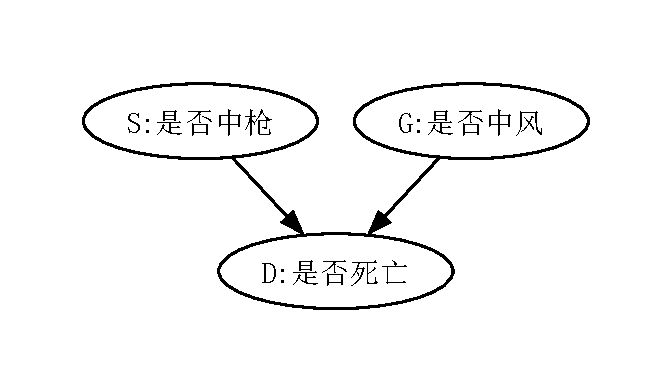
\includegraphics[width=0.5\textwidth]{image/对撞路径例子.pdf}}
	\caption{伯克森悖论}
	\label{fig:berkson}
\end{figure}

图\ref{fig:berkson}中展示了一例:众所周知,枪击和中风都会导致生命的消散,但是人的生命只有一次也不能复活,因而如果一定要死(也就是这两种死法),也只能够选择其中一种,显然,被枪打死的人不可能再中风死,在观察时若我们如果只看到死在这两种死法下的个体,则轻易可以得出中枪死与中风死有着负向相关的关系。

\paragraph*{辛普森悖论(Simpson’s Paradox)}是统计学中著名的聚合现象,指数据在整体层面呈现某种趋势,但按某一变量分层后,各子组的趋势方向与整体相反。

\begin{figure}[ht]
	\centering
	\fbox{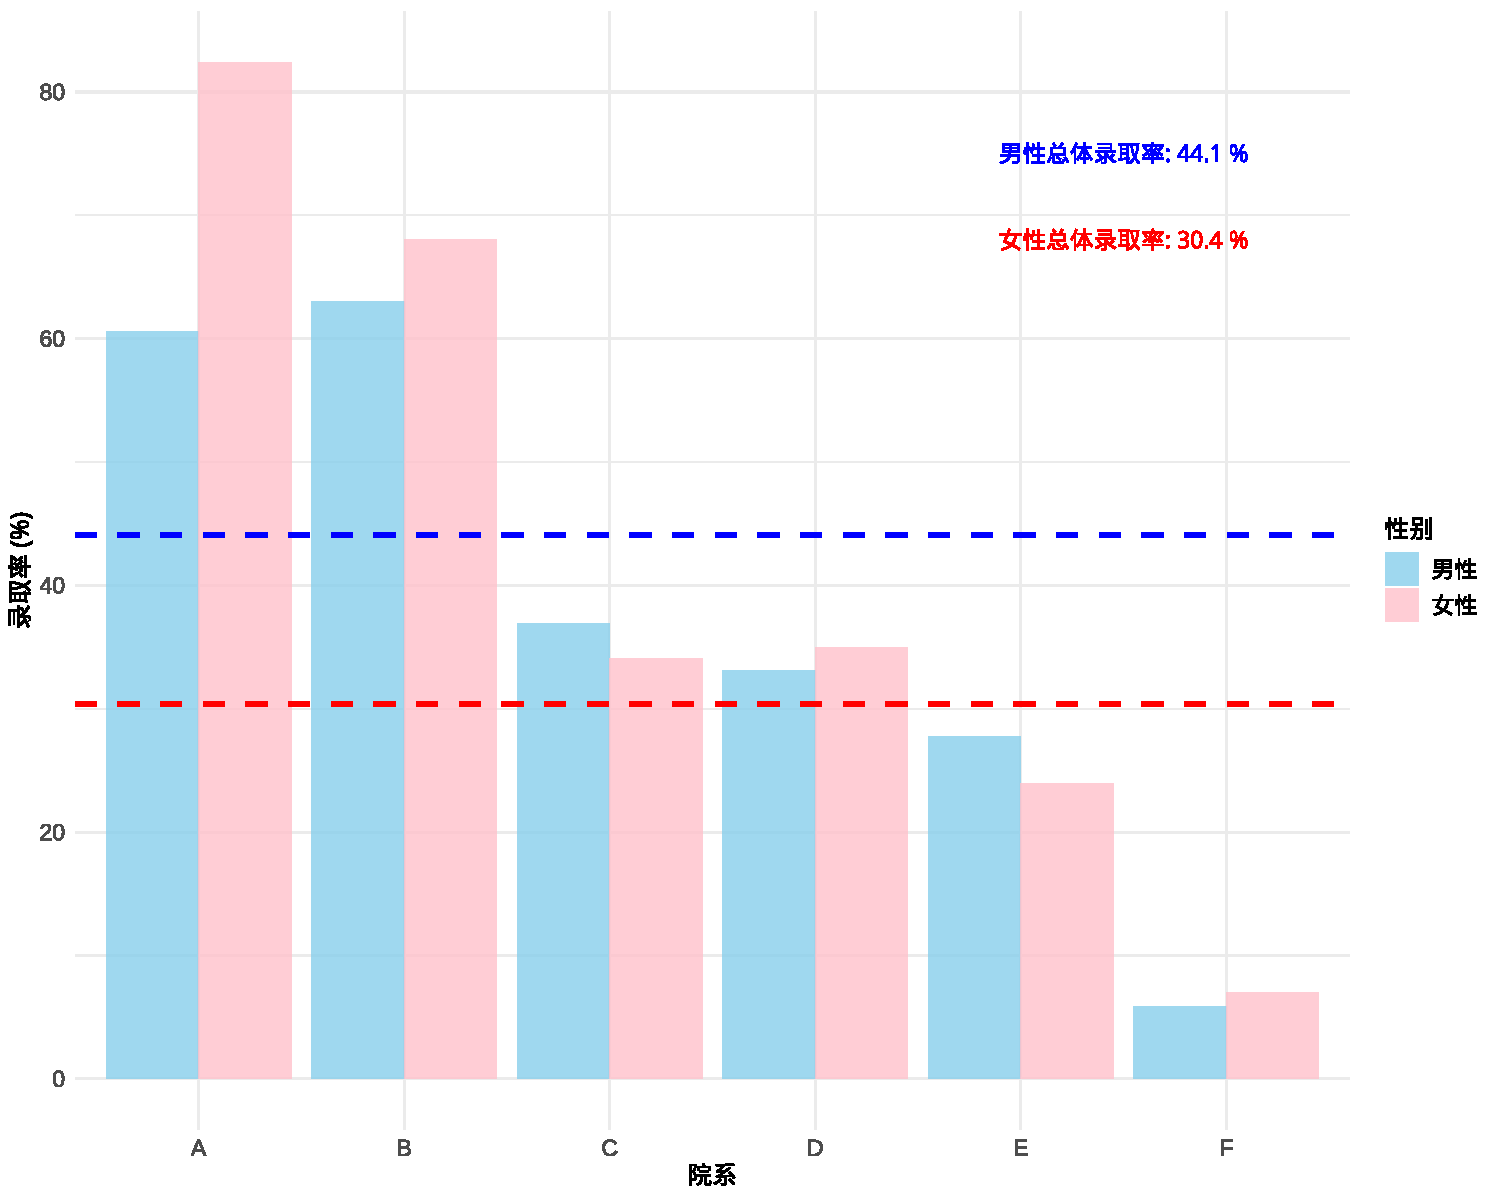
\includegraphics[width=0.5\textwidth]{image/simpson_paradox.pdf}}
	\caption{辛普森悖论}
	\label{fig:simpson}
\end{figure}

典型案例即为伯克利研究生院性别录取率差异,总的来看,男性的录取率高于女性(44.1\%大于30.4\%),但当我们把研究生院再划分为不同的院系后,大部分院系对于女性的录取率实际高于男性(见图\ref{fig:simpson})。彼得·比克尔(Peter Bickel)认为这一现象乃处于女性更倾向于申请竞争压力较大的院系,在这种情况下,大量的陪跑案例当然拉低了总的录取率。该悖论揭示了忽视混杂变量可能导致的错误推论,强调分层分析与因果推断中考虑潜在混杂因素的必要性。

\paragraph*{罗德悖论(Lord’s Paradox)}指同一数据集通过不同统计方法分析可能得出矛盾结论的现象。这一悖论最早由统计学家弗雷德里克·罗德(Frederic Lord)在1967年提出,揭示了数据分析中一个关键问题:统计方法的选择如何影响研究结论,尤其是在涉及协变量调整时。

\begin{figure}[ht]
	\centering
	\fbox{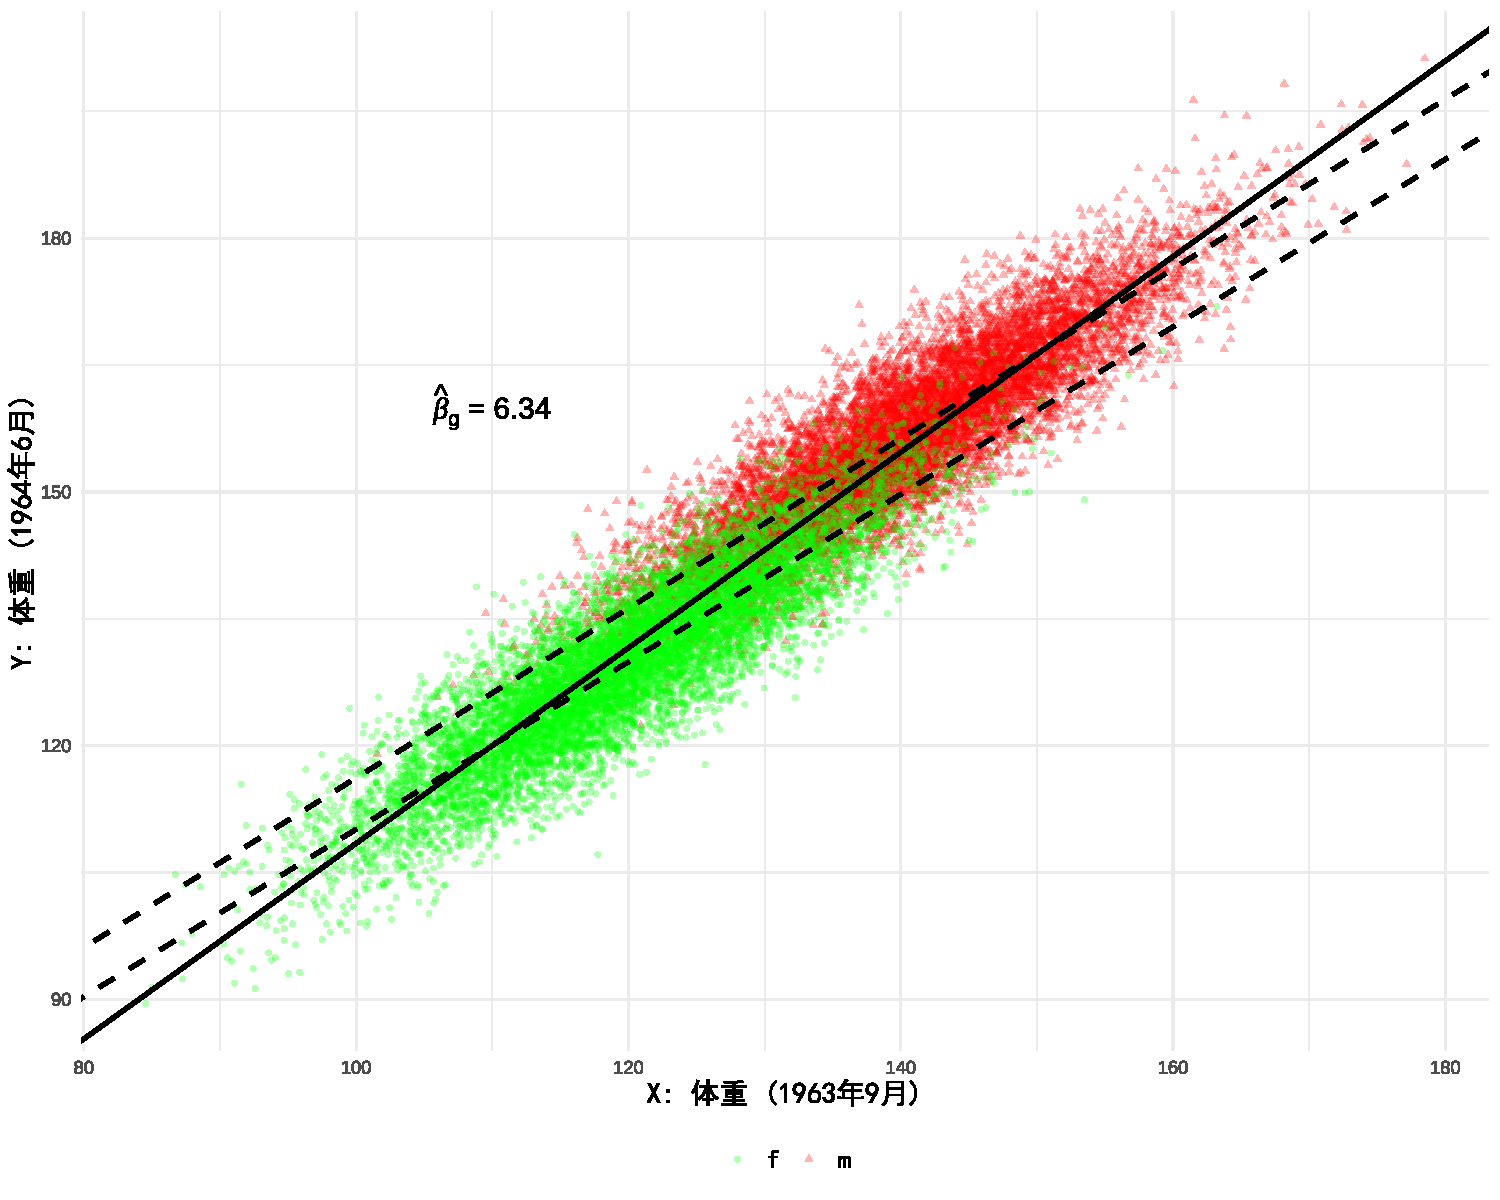
\includegraphics[width=0.5\textwidth]{image/lords_paradox.pdf}}
	\caption{罗德悖论}
	\label{fig:lord}
\end{figure}

在罗德的研究案例中,两位统计学家对同一组数据(学生入学体重X和一年后体重Y,图\ref{fig:lord})进行分析,却得出截然相反的结论:

\begin{enumerate}
	\item 简单均值比较:第一位统计学家直接比较男女学生的体重变化均值,发现两组均无显著变化,因此认为食堂对体重无影响。
	\item 协方差分析(ANCOVA):第二位统计学家学过控制入学体重(X)后,发现男女学生的体重变化存在显著差异(截距差为6.34磅),认为食堂对男女影响不同。
\end{enumerate}

这一矛盾表明,是否调整协变量可能导致研究结论的差异,其背后的根本问题在于,我们无法得知不吃食堂这一反事实(counterfactual)条件下男女的体重情况(没有对照组),因而使得回归或者协方差分析等统计工具失效,并不能清楚地回答有关因果的问题。

通过因果图的形式,我们可以更直观地看到这些悖论的出现,此处可以跳到图\ref{fig:relation}复习。显然,这些变量关系在本章中又再次出现,由于已经引入了因果图的概念,我们可以对其进行案例化,如图\ref{fig:wahaha}:

\begin{figure}[ht]
	\centering
	\fbox{
\includegraphics[width=0.5\textwidth]{image/wahaha.png}}
	\caption{财产分配的因果图}
	\label{fig:wahaha}
\end{figure}

在某企业家引发的舆情事件中,我们尝试提炼出一个关于社会关系继承的因果机制模型。首先,从死亡方式切入,该企业家据称因病去世(例如中风),这一前提将我们讨论的问题限定在“自然死亡”或“疾病死亡”等非暴力性死亡情境之中。这一设定本身即排除了如枪击等“非自然死亡”情境所涉及的诸多干扰因素,从而有助于厘清自然死亡背景下的社会关系变动,当然我们在做大样本分析时不能排除非自然死亡的情况。

然而,在因果分析中一旦引入“是否死亡”作为控制变量,便可能无意间触发“\textbf{对撞偏差}”(collider bias)的问题:当一个变量(如“是否死亡”)同时受到两个原本无关联的因素(如“是否中风”与“是否枪击”)影响,且被纳入分析模型时,会在它们之间引入人为关联,从而扭曲对因果路径的识别。例如,死亡作为既成事实,是我们观察遗产分配问题的前提,而死亡方式作为路径条件,本应是划定分析边界的工具。但当我们将“是否死亡”作为控制变量时,原本独立的“是否中风”与“是否枪击”两个变量便在图式中联通,形成类似“ $ \text{是否中风} \rightarrow \text{是否枪击} \rightarrow \text{确立遗嘱}$ ”这样的虚假因果路径。这种结构性错误会削弱我们对“自然死亡背景下遗嘱确立行为”这一主路径的识别能力。

进一步而言,“确立遗嘱”通常通过影响“家庭关系”间接作用于“财产分配”,家庭关系因而可被视作一个具有机制意义的中介变量。该路径结构揭示出财产继承不仅是个人意愿的体现,也是亲属关系结构的延续与反映。然而,若研究者试图将所有可能的中介路径一并纳入模型进行调整(例如控制家庭互动频率、情感亲疏、文化观念等),则可能落入“\textbf{过度控制偏差}”(over-control bias)的陷阱。在这种情况下,“个人意愿”这一关键变量的真实效应,可能被其他解释变量的残差结构所吸收,从而妨碍我们对主因路径的识别与估计。

在死因探讨之外,“日常为人”(例如企业家的性格、道德声誉、人际互动方式等)不仅可能影响其家庭关系,也可能对其财产分配产生前因上的作用。因此,“日常为人”作为一个潜在混淆变量,若未被纳入分析,将可能引发如“辛普森悖论”这类由于聚合数据忽视分层关系而造成的推断错误,也叫“\textbf{混淆偏差}”(confusion bias)。

此外,不容忽视的是“法律制度”等宏观背景变量。虽然其通常具有高度稳定性,短期内不易观察其变化,但在长时段演化中,其对遗嘱制度与财产分配的规范作用不可忽略。尽管制度或文化等外在环境因子的量化困难重重,但已有研究通过创新方法成功应对这一挑战。

\subsection{截断}

面对上述的复杂因果关系,我们似乎难以把握,尤其是如何精准地提取出X对Y的影响。事实上,指望在统计学范畴内予以彻底解决——尤其是在社会科学领域中试图收集关于全体变量的完备数据——几乎是不可能的任务。正因如此,珀尔提出了“干预主义”思想,并以do算子为工具,试图跳出被动观察的框架,主动设定变量的状态,从而厘清因果路径。

然而,即便引入了干预操作,我们仍需回答一个基础性问题:在干预变量X的同时,是否还有其他路径会影响到Y?亦即,我们如何“截断”所有除 $X \rightarrow Y$ 之外的混杂路径,只保留真正的因果链?为此,理解路径结构是至关重要的,以下两类共四种路径类型构成了因果图分析的基础。

\paragraph*{前门路径}

前门路径指的是一种通过中介变量传导的路径,即存在一条 $X \rightarrow M \rightarrow Y$ 的路径,其中M是介于X与Y之间的中介变量。若前门路径独立于所有混杂路径,并且X对M与M对Y的因果关系均可识别,那么通过控制M这一中介变量,即可在未观测混杂变量Z的前提下识别 $X \rightarrow Y$ 的因果效应。这便是所谓“前门准则”(front-door criterion)所依赖的结构条件。

在上述的例子当中,当我们认定生前为人对家庭关系并无影响的情况下,便可以通过估测是否死亡对家庭关系( $X \rightarrow M$ )以及家庭关系对遗产分配( $M \rightarrow Y$ )得出一个确立遗嘱对遗产分配( $X \rightarrow Y$ )的因果效应来。

前门路径的核心优势在于:它不要求我们观测并控制所有影响 $X$ 和 $Y$ 的共同原因,而是通过中介变量的“结构绕行”实现了因果推断。这也体现出结构因果模型(SCM)在非实验数据中的强大推理能力。

引入do算子之后,我们关注的已不再是观察性条件概率 $P(Y \mid X)$,而是介入性概率 $P(Y \mid do(X))$。这是因为 $do(X)$ 表示我们人为地设定变量 $X$ 的值,从而切断 $X$ 与其上游变量(包括潜在混杂变量 $Z$)之间的自然因果联系。这一操作是实现因果推断的关键步骤。

在满足前门准则的前提下,$P(Y \mid do(X))$ 可以通过如下公式进行识别:

\begin{equation}
P(Y \mid do(X)) = \sum_{m} P(M = m \mid X) \sum_{x'} P(Y \mid M = m, X = x') P(X = x')
\end{equation}

这一表达式背后的逻辑如下:我们首先利用 $P(M \mid X)$ 捕捉 $X$ 对中介变量 $M$ 的因果影响,然后通过对所有可能的 $x'$ 求和来消除 $X$ 与 $M$ 之间的关联性,进而评估 $M$ 对 $Y$ 的因果影响。由于 $M$ 同时受到 $X$ 的影响并影响 $Y$,其在传导因果效应的过程中起到了桥梁作用。

继续回到前述的社会情境例子,在认为“为人”不影响“家庭关系”的前提下,如果我们能观测并建模“是否立遗嘱”对“家庭关系”的影响($X \rightarrow M$),以及“家庭关系”对“遗产分配”的影响($M \rightarrow Y$),则即便存在无法观测的混杂变量(例如家族文化、遗产规模、潜在冲突历史等),但由于这些混杂变量不直接影响到家庭关系这一中介变量,故我们仍可以通过前门准则识别 $X$ 对 $Y$ 的净因果效应,如图\ref{fig:wahaha2}所示。

\begin{figure}[ht]
	\centering
	\fbox{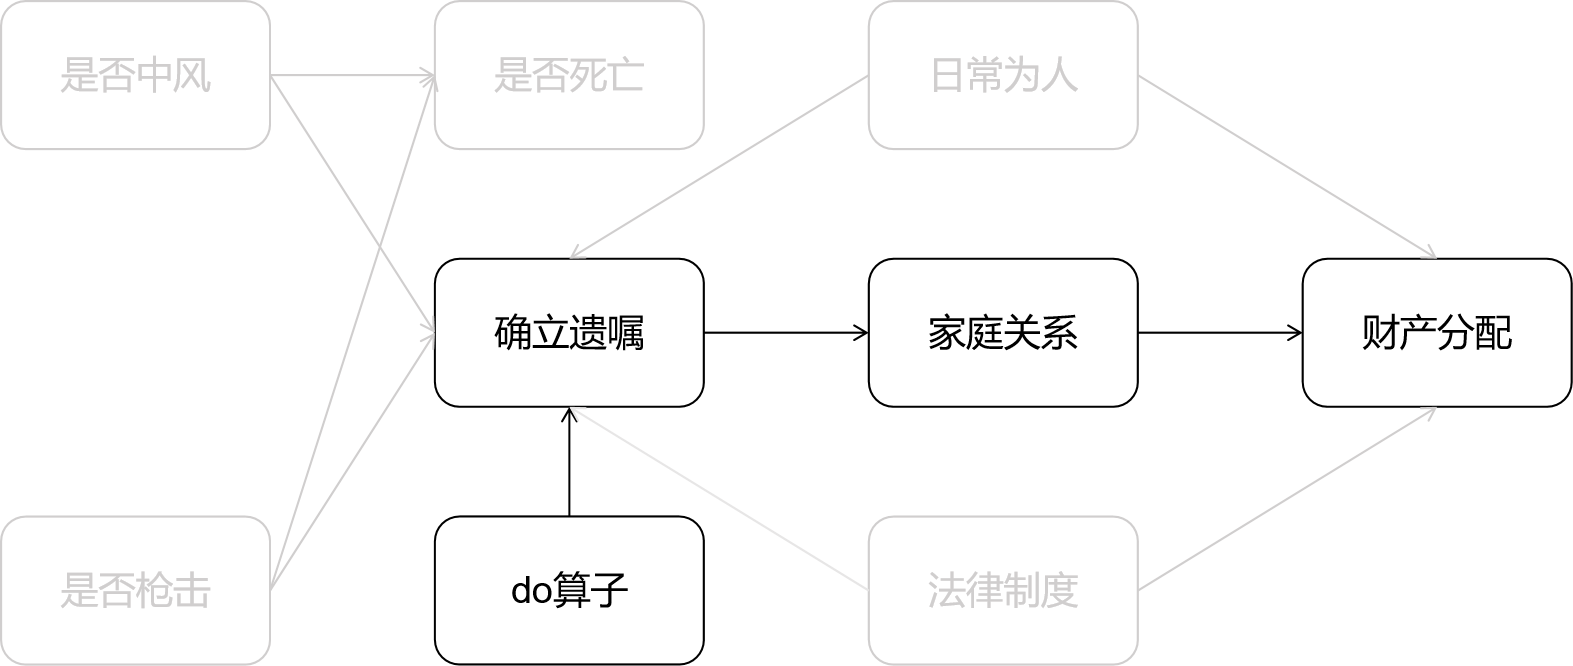
\includegraphics[width=0.5\textwidth]{image/wahaha2.png}}
	\caption{前门路径示例图}
	\label{fig:wahaha2}
\end{figure}

\paragraph*{后门路径}

相比之下,后门路径是一条从 $X$ 开始,并通过其他变量“绕道”影响 $Y$ 的路径,但其首个箭头是指向 $X$ 的,例如 $X \leftarrow Z \rightarrow Y$。这样的路径通常并不代表真正的因果传导链条,而是一条混杂路径(confounding path),会引入 $X$ 与 $Y$ 之间的虚假相关性,从而干扰我们对 $X \rightarrow Y$ 因果效应的识别。

为了封闭此类路径,我们需要控制这些共同前因(common causes),即将变量 $Z$ 纳入模型作为控制变量,使得在条件化 $Z$ 之后,$X$ 与 $Y$ 之间的关联可以被解释为因果效应。如图\ref{fig:wahaha3} 示,在我们的实际社会例子中,“日常为人”与“法律制度”可能既影响立遗嘱的行为,也影响财产分配的结果,因此构成混杂变量,需予以控制。

珀尔提出的“后门准则”(back-door criterion)是识别这类因果效应的重要工具。具体而言,若存在一个变量集合 $\mathbf{Z}$ 满足:

\begin{itemize}
	\item 所有从 $X$ 到 $Y$ 的后门路径都被 $\mathbf{Z}$ 所阻断;
	\item $\mathbf{Z}$ 不包含任何 $X$ 的后果(即不包括 $X$ 的子节点,否则变为内生性问题)。
\end{itemize}

则因果效应 $P(Y \mid do(X))$ 可通过如下方式识别:

\begin{equation}
P(Y \mid do(X)) = \sum_{z} P(Y \mid X, Z = z) P(Z = z)
\end{equation}

在该表达式中,$P(Y \mid X, Z)$ 是在观测数据中可以直接估计的条件概率,而 $P(Z)$ 是混杂变量的边际分布。通过对所有 $z$ 的加总,我们相当于模拟了一个“随机赋值” $X$ 的实验情境,从而排除了由于 $Z$ 引起的混杂偏误。

需要特别强调的是,这一公式的左侧为 $P(Y \mid \mathbf{do}(X))$,表示我们关心的是在人为地干预 $X$ 为某一特定值时,$Y$ 的响应分布——这是因果推断的核心目标。右侧虽然只涉及观察性概率(即没有 $do$),但由于我们通过控制混杂变量 $Z$ 封闭了所有非因果路径,进而使得 $P(Y \mid X, Z)$ 可以作为 $X \rightarrow Y$ 因果效应的替代估计。

换言之,这一加权求和过程相当于在每个 $Z=z$ 的条件下估计 $X$ 对 $Y$ 的局部因果效应,并按 $Z$ 的边际分布 $P(Z)$ 进行整合,从而还原出全局的干预效应 $P(Y \mid \mathbf{do}(X))$。通过这种方式,我们实现了从观察性数据中“模拟实验”,使得不具备随机化条件的数据也能够进行有效的因果识别。

后门准则的实质是:在能够观测并控制混杂变量的前提下,我们可以通过调整(adjustment)还原出一个近似实验的因果估计。而do算子的引入则使得这种估计从统计相关性上升为因果推断。


\begin{figure}[ht]
	\centering
	\fbox{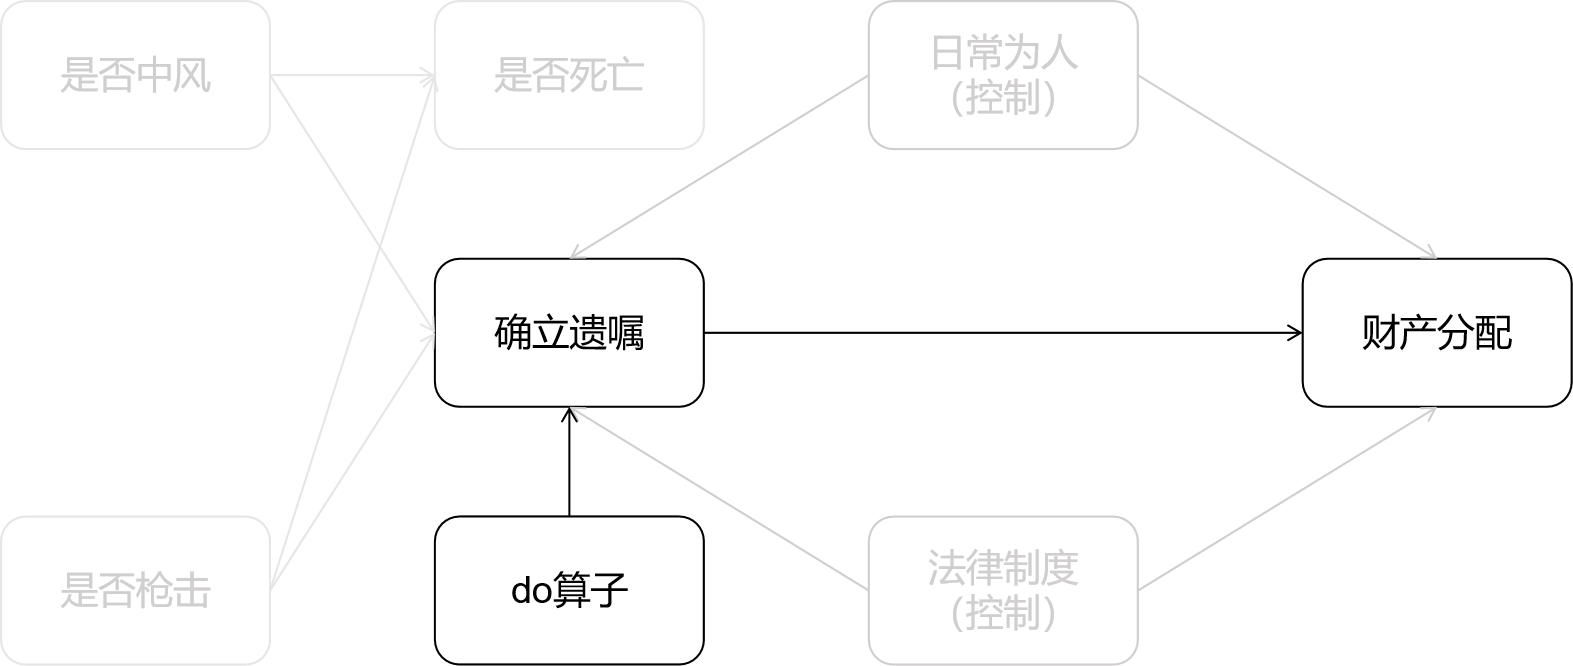
\includegraphics[width=0.5\textwidth]{image/wahaha3.png}}
	\caption{后门路径示例图}
	\label{fig:wahaha3}
\end{figure}

\paragraph*{开路径}

所谓“开路径”是指一条变量之间的路径,其结构在没有被控制的前提下,允许信息在变量间流通,从而导致相关性。在因果图中,如果路径中的所有非冲节点(collider)未被控制,且没有冲节点的后代被控制,那么这条路径就是“开”的(也就是因果图中因能走向果)。这意味着X与Y之间可能因该路径而存在关联,尽管这种关联未必具有因果含义。因此,在识别因果关系时,必须将所有不希望开启的路径加以“\textbf{截断}”。

\paragraph*{死路径}

与“开路径”相对,死路径指的是在控制某些变量后,使路径上出现冲节点或其后代,从而阻断信息流通的一条路径。典型的死路径形式是当路径中存在冲节点(如 $X \rightarrow W \leftarrow Y$)且未控制W或其后代时,该路径自动封闭,变量之间不再相关。对撞路径实际上便是一条死路经,显然,“是否中枪”与“是否中风”的关联完全是由于死亡这一结果而出现,两者间实际上并无瓜葛。这一特性在因果识别中尤为关键,因为它说明并非所有路径都需要控制,有些路径由于结构上的封闭性天然为“死路径”,不构成混杂来源,控制其反而造成“对撞偏差”。

尽管珀尔的理论如此完备,想要据此寻找可行的前门路径和截断所有后门路径仍然不太可能,结构式的复杂也在此凸显无疑,当下的计量经济学似乎是,也仍然将是简约式的主场,通过设计,我们实现了在找不齐路径中变量的情况下仍然能控制偏差的壮举。

\subsection{设计}

现代因果推断的思想萌芽可以追溯到19世纪,但其形式化理论的奠基主要发生在20世纪。回顾林德医生的实验,其核心逻辑——通过人为控制变量,比较处理与非处理之间的差异——与现代实验设计高度一致。这种逻辑,正是后世“潜在结果框架”(Potential Outcomes Framework)所要精确表达的内容。

这一框架的发展历经了数位巨擘的奠基。因此,它通常被称为“奈曼—鲁宾因果模型”(Neyman-Rubin Causal Model, RCM)。其发展脉络清晰地体现了理论的演进:

\begin{itemize}
    \item 耶日·奈曼 (Jerzy Neyman, 1923) 在其关于农田实验的研究中,首次引入了“潜在结果”的数学符号,用以定义不同处理下的潜在产量。这为因果效应的量化提供了数学语言,但当时仅限于随机化的实验场景。
    \item 罗纳德·费舍尔 (Ronald Fisher, 1925) 提出了将处理“随机化”分配给单元是进行因果推断的“合理基础”。他强调了物理随机化在创造可比组别、消除系统性偏差方面的核心作用,使随机对照实验(RCT)成为因果推断的“黄金标准”。
    \item 唐纳德·鲁宾 (Donald Rubin, 1974) 将潜在结果框架从纯粹的实验环境推广至观察性研究,使其成为一个普适的因果分析工具。他明确指出,无论数据来源如何,因果效应的核心定义都应基于潜在结果的比较,并正式提出了“分配机制”在因果识别中的重要性。
\end{itemize}

\paragraph*{核心概念}

鲁宾因果模型的核心构件包括三个基本概念:干预 (Treatment)、潜在结果 (Potential Outcome)与干预效应 (Treatment Effect)。

\begin{itemize}
    \item \textbf{干预}:指研究中所施加的某种处理或变化,通常是我们试图识别其因果影响的自变量。
    \item \textbf{潜在结果}:指在不同干预状态下,一个研究对象可能产生的因变量取值。例如,$Y_i^1$ 表示单位 $i$ 接受处理后的结果,$Y_i^0$ 表示其未接受处理(处于对照状态)的结果。
    \item \textbf{干预效应}:即同一单位在两种状态下潜在结果的差值,是我们最终希望估计的因果量。
\end{itemize}

该框架揭示了被霍兰德(Paul Holland)称为的所谓的“因果推断的根本问题”(Fundamental Problem of Causal Inference, FPCI):对于任一研究对象,在特定时间内只能处于一种处理状态,因此我们永远只能观察到一个潜在结果,另一个则永远处于未被观察到的反事实状态。这种结构性的“数据缺失”是因果分析的核心挑战。

\paragraph*{估计目标}

根据作用层级的不同,干预效应可分为个体层面与总体层面。

\begin{itemize}
    \item 个体干预效应 (ITE, Individual Treatment Effect)指单位 $i$ 在接受干预与未接受干预状态下结果之差。由于FPCI,该值无法直接观测。
    \begin{equation}
        \delta_i = Y_i^{1} - Y_i^{0}
    \end{equation}
    \item 平均处理效应 (ATE, Average Treatment Effect)是最常用的总体参数,定义为所有个体效应的期望值。
    \begin{equation}
        \delta_{ATE} = E[Y_i^1 - Y_i^0]
    \end{equation}
    \item 处理组的平均处理效应 (ATT, Average Treatment Effect on the Treated)关注处理对实际接受者的平均影响。
    \begin{equation}
        \delta_{ATT} = E[Y_i^1 \mid D_i = 1] - E[Y_i^0 \mid D_i = 1]
    \end{equation}
    \item 控制组的平均处理效应 (ATU, Average Treatment Effect on the Untreated)关注处理对未接受者的潜在平均影响。
    \begin{equation}
        \delta_{ATU} = E[Y_i^1 \mid D_i = 0] - E[Y_i^0 \mid D_i = 0]
    \end{equation}
\end{itemize}

其中,$D_i=1$ 表示个体 $i$ 接受处理,$D_i=0$ 表示未接受处理。

\paragraph*{核心假设}
为了克服 FPCI 并从观测数据中估计因果效应,我们需要依赖一系列关键假设。

\begin{enumerate}
    \item \textbf{稳定单元处理值假设 (SUTVA, Stable Unit Treatment Value Assumption)}:此假设包含两个方面:
    \begin{itemize}
        \item 无干扰,即一个个体的处理状态不会影响其他个体的潜在结果;
        \item 处理无多重版本,即处理的实现方式对所有接受者都是一致的。
    \end{itemize}
    \item \textbf{可忽略性/非混淆性假设 (Ignorability / Unconfoundedness Assumption)}:这是连接潜在结果与观测数据的桥梁。它要求处理的分配独立于潜在结果,在给定一组协变量 $X$ 的条件下。形式化表示为:$(Y_i^1, Y_i^0) \perp D_i \mid X_i$。在随机实验中,由于物理随机化,该假设自然成立(无需条件化)。在观察性研究中,研究者必须通过控制所有相关的混淆变量来尽可能满足此假设。
\end{enumerate}

当这些假设满足时,我们就可以用控制组的观测结果来估计处理组的反事实结果,从而识别因果效应。例如,在满足可忽略性假设时,$E[Y_i^0 \mid D_i = 1] = E[Y_i^0 \mid D_i = 0]$,ATT的估计就成为可能。

\paragraph*{实验设计}
在理想情境下,随机对照实验(RCT)因其能够满足非混淆性假设而被视为“黄金标准”。然而,在社会科学中,由于伦理、成本或操作复杂性,严格的RCT往往难以实施。因此,研究者发展了多种实验设计样式以应对复杂现实。

\begin{itemize}
    \item \textbf{被试间设计 (Between-Subject Design)}:将被试随机分配至互斥的处理组与对照组。这是最经典的设计,其变体包括:
    \begin{itemize}
        \item 前测—后测控制组设计:比较处理前后的变化,控制时间趋势。
        \item 仅后测设计:适用于无法或不宜实施前测的场景。
        \item 所罗门四组设计:综合前两者,用以评估并控制前测本身带来的效应。
    \end{itemize}
    \item \textbf{被试内设计 (Within-Subject Design)}:每个受试者依次接受所有处理条件。该设计能完美控制个体间异质性,但需警惕顺序效应(如学习、疲劳效应)。
\end{itemize}

无论何种设计,其首要目标都在于提升\textbf{内部效度},即确保观测到的因果关系确实来自处理本身。然而,过于理想化的实验可能脱离现实,损害结论的\textbf{外部效度}(泛化能力)。因此,如实地实验 (Field Experiment)等设计,试图在自然情境中施加干预,以求在内部效度与外部效度之间取得平衡。

当严格的实验不可行时,社会科学研究者更多依赖观察性数据,并发展出从自然实验 (Natural Experiments)到准实验 (Quasi-Experiments)等一系列方法,试图在“戴着镣铐跳舞”的条件下,尽可能逼近因果推断的理想状态。

\section{从统计推断到因果推断}

理解因果关系是社会科学的核心任务。传统统计推断在描述相关性方面表现出色,但在揭示因果机制时却面临根本性局限。现代计量经济学试图填补从统计相关到因果推断的鸿沟,其基本目标是在有限的数据约束下,通过形式化建模揭示变量间的因果联系,并对特定政策或干预的效果做出可靠估计。

实践中,计量研究多依赖于观察性数据。其最大特征在于,研究者无法控制处理变量的分配机制,因此极易受到混淆因素的干扰。在这种情形下,内生性成为因果推断最关键的挑战。内生性主要源于三个方面:遗漏变量、测量误差以及互为因果。为了应对这些挑战,计量经济学发展出两大核心分析框架:基于匹配的推断路径与基于回归的推断路径。

\subsection{基于回归的因果推断路径}

回归是社会科学与计量经济学中最为经典的因果推断工具之一。其基本思想是刻画变量之间的条件期望关系,并在此基础上识别出解释变量的因果效应。回归框架的优势在于,它不仅能够通过参数化建模来控制混淆变量,还能够与自然实验或准实验设计相结合,以分离出外生的变动部分。因此,回归分析既是一种描述性方法,也是因果推断的核心工具。

\textbf{线性回归模型}:普通最小二乘法(OLS)是回归分析的起点。其估计建立在零条件均值假设之上,即 $\mathbb{E}[\varepsilon|X]=0$ 这意味着解释变量与误差项不相关。在该假设成立时,OLS估计量不仅无偏一致,而且回归系数可被解释为控制其他变量后,自变量变化对因变量的边际效应。线性回归的灵活性在于,它可以通过加入控制变量来削弱遗漏变量偏误,并通过交互项、非线性变换等方式拓展模型的表达能力。然而,如果零条件均值假设被违反,例如存在遗漏变量、测量误差或反向因果关系,则OLS系数将不再具有因果解释。

\textbf{面板数据模型}:当数据在个体与时间两个维度上同时存在时,面板数据模型成为控制未观测异质性的有力工具。  
\begin{itemize}
    \item \textbf{固定效应模型(FE)}通过引入个体虚拟变量,剥离了所有随时间不变的个体特征,从而避免这些不随时间变化的混淆因素影响估计。
    \item \textbf{随机效应模型(RE)}则假设个体效应是随机的,且与解释变量独立。在该假设成立时,RE能够更高效地利用样本内外的变异。
\end{itemize}

\textbf{工具变量法(IV)}:当解释变量内生时,OLS不再能识别因果效应。此时,工具变量法提供了一个解决方案。一个合格的工具变量必须满足两个条件:

\begin{itemize}
	\item 相关性:工具变量与内生解释变量高度相关;
	\item 外生性:工具变量对结果变量的影响仅通过内生解释变量发挥作用。
\end{itemize}

基于工具变量的\textbf{两阶段最小二乘法(2SLS)}是标准的估计方法。近年来,局部平均处理效应(LATE)的提出进一步澄清了IV估计的识别含义,强调其揭示的是特定人群的“边际个体”效应。

\textbf{准实验设计}:当RCT在实际操作中不可行、成本过高或在伦理上不被允许时,研究者往往会转而利用现实世界中自然发生的“类实验”情境,来识别因果效应。这些方法统称为准实验设计。与RCTs通过研究者主动干预并随机分配处理组和对照组来确保两者在处理前无系统性差异不同,准实验设计则是在非随机分配处理的情况下,通过巧妙的统计方法和识别策略,尽可能地模拟随机化实验的条件,从而从观测数据中抽取出处理变量的因果效应。

\begin{itemize}
    \item \textbf{双重差分法(DID)}专为评估政策或事件冲击而设计,其核心假设是“平行趋势”,即在没有处理的情况下,处理组与对照组应具有相同的时间演化趋势。
    \item \textbf{断点回归设计(RDD)}适用于处理状态由某一连续变量是否超过阈值决定的情境。其关键假设是,在阈值附近个体具有相似特征,因此处理效应可通过阈值两侧的结果差异识别。
    \item \textbf{合成控制法(Synthetic Control)}常用于政策干预的跨区域比较,通过构造一个“合成的对照组”来识别干预效应。
\end{itemize}

\subsection{基于匹配的因果推断路径}

与回归方法不同,匹配方法不依赖于参数化的函数形式假设,而是通过在处理组与对照组之间寻找协变量特征相似的个体进行配对,从而构造一个可比的对立事实。这一方法强调“在可比的个体之间做比较”,以尽可能消除协变量差异带来的选择性偏误。

\textbf{处理效应}:因果推断的核心目标是估计处理效应,即比较同一个体在接受与未接受处理时的结果差异。由于反事实结果不可观测,匹配方法通过寻找“替身”来近似这一比较。常见的处理效应指标包括:平均处理效应(ATE)、处理组的平均处理效应(ATT)、以及条件平均处理效应(CATE)。

\textbf{倾向得分匹配(PSM)}:在高维协变量空间下,直接进行多维匹配非常困难。倾向得分匹配通过估计每个个体接受处理的概率(即倾向得分)来降低维度复杂性。其逻辑为:若在给定倾向得分的条件下,处理分配与结果独立(条件可忽略性假设),则匹配基于倾向得分即可实现因果识别。常见方法包括最近邻匹配、卡钳匹配和核匹配等。

\textbf{匹配的优势与局限}:匹配方法的优势在于其非参数性质,不依赖于线性或特定函数形式的假设,且结果直观易于解释。然而,它也存在明显局限:  
\begin{itemize}
    \item 匹配仅能控制基于可观测变量的选择偏误,无法消除不可观测因素的影响;
    \item 匹配质量高度依赖于协变量的丰富性与重叠性,若缺乏共同支持区间,结果可能偏误;
    \item 在样本有限的情况下,匹配可能带来效率损失。
\end{itemize}

总体而言,回归与匹配代表了现代因果推断中的两类互补路径。回归通过建模来控制混淆因素,并结合准实验设计处理内生性问题;匹配则通过数据预处理直接构造可比组,强调非参数和直观性。在实证研究中,二者常常结合使用:研究者可先通过匹配消除处理组与对照组在协变量分布上的差异,再利用回归模型进行进一步调整,从而获得更为稳健和可靠的因果推断结果。这种“多工具并用”的思路,已成为现代因果推断实践中的常态。

后文将对每一段进行细致地展开,并配有Stata代码案例,基本格式如下:

\begin{tcolorbox}[title=Stata 示例, colback=white, colframe=black, colbacktitle=white, coltitle=black,fonttitle=\bfseries]
 * Stata 输入
	\begin{lstlisting}[xleftmargin=2em]
	quietly sysuse auto, clear // 加载系统自带数据集
	summarize // 描述性统计
	graph bar weight price, over(foreign) // 绘制分组条形图
	\end{lstlisting}
 * Stata 输出
	\vspace{-2em}
	\begin{Verbatim}[commandchars=\\\{\},xleftmargin=2em]

		
    Variable |        Obs        Mean    Std. dev.       Min        Max
-------------+---------------------------------------------------------
        make |          0
       price |         74    6165.257    2949.496       3291      15906
         mpg |         74     21.2973    5.785503         12         41
       rep78 |         69    3.405797    .9899323          1          5
    headroom |         74    2.993243    .8459948        1.5          5
-------------+---------------------------------------------------------
       trunk |         74    13.75676    4.277404          5         23
      weight |         74    3019.459    777.1936       1760       4840
      length |         74    187.9324    22.26634        142        233
        turn |         74    39.64865    4.399354         31         51
displacement |         74    197.2973    91.83722         79        425
-------------+---------------------------------------------------------
  gear_ratio |         74    3.014865    .4562871       2.19       3.89
     foreign |         74    .2972973    .4601885          0          1
	\end{Verbatim}

	\begin{center}
	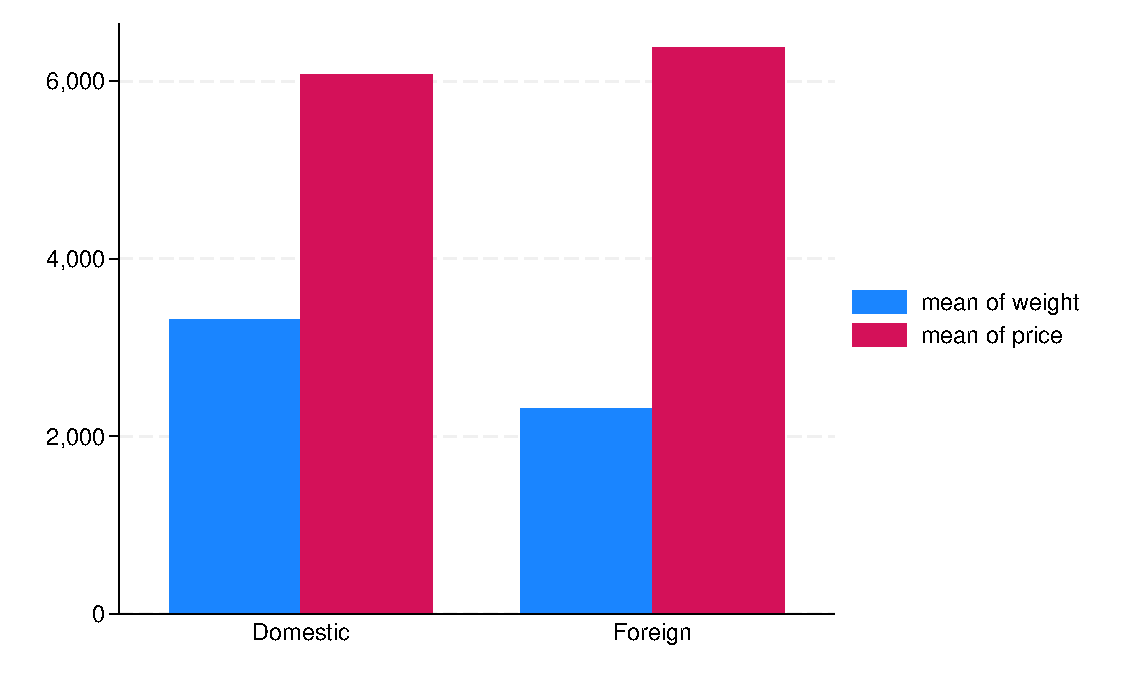
\includegraphics[width=0.8\textwidth]{image/autobar.pdf}
	\end{center}

\end{tcolorbox}

\newpage
\thispagestyle{empty}
\begin{thebibliography}{99}
	\bibitem{1}
	邱嘉平,《因果推断实用计量方法》,上海财经大学出版社

	\bibitem{2}
	赵西亮,《基本有用的计量经济学》,北京大学出版社

	\bibitem{3}
	珀尔 \ 等,《为什么》,中信出版集团

	\bibitem{4}
	安格里斯特 \ 等,《基本无害的计量经济学》,格致出版社

	\bibitem{5}
	游宇 \ 等.一切为了理论——理论化与整合性的案例选择策略[J].世界经济与政治, \\ 2023,(12)

	\bibitem{6}
	许琪.因果推断五十年:成就、挑战与应对[J].学术月刊,2024,56(11)

    \bibitem{7}
	因本斯 \ 等,《因果推断导论》,格致出版社

	\bibitem{8}
	燕继荣 \ 等,《发展政治学学科地图》,北京大学出版社

\end{thebibliography}
\chapter{统计推断的理解运用}

\section{多元回归}

\subsection{数据生成过程}

\textbf{基本概念}  

科学研究的核心在于揭示数据背后的生成机制。可知论认为宇宙的运行遵循特定规律,这些规律决定了观测数据的生成方式。这种支配数据生成的潜在机制被称为\textbf{数据生成过程(Data Generating Process, DGP)},它是进行统计推断和因果分析的基础。

DGP是一组隐藏在数据背后的规律性法则。虽然我们无法直接观测这些法则,但能通过其产生的数据进行反向推导。例如,当物体自由下落时,我们观察到的是下落现象,而支配这一现象的本质规律——重力,正是该过程的DGP组成部分。

\textbf{自然科学中的应用} 

以牛顿万有引力定律为例,其数学表达式为:  
\begin{equation}
    F = G \frac{m_1 m_2}{r^2}
\end{equation}  
其中$G$为万有引力常数,$m_1$、$m_2$为物体质量,$r$为距离。这个方程揭示了天体运动背后的DGP。牛顿正是通过观测行星轨迹数据,成功推导出这一规律,从而揭示了引力作用的本质。

\textbf{社会科学中的应用}  

相较于自然科学,社会科学的DGP通常具有更强的复杂性与不确定性。但只要承认观测数据存在某种程度的规律性,就必然存在对应的DGP。理解DGP的关键在于把握两个维度:  
\begin{enumerate}
    \item \textbf{已知规律}:利用既有知识指导数据分析
    \item \textbf{未知规律}:通过研究揭示新的规律性
\end{enumerate}  

以发色与收入的关系研究为例,掌握DGP有助于控制混杂因素(如教育水平、职业选择等),从而获得更精准的因果效应估计。研究者可通过设定特定DGP生成模拟数据,这种"上帝视角"的数据构建方式能完整掌控生成机制,为方法验证提供理想实验环境。例如在收入研究中,可设定:

\begin{itemize}
    \item 收入服从对数正态分布
    \item 棕发群体收入提升10\%
    \item 20\%人口天生棕发
    \item 大学学历带来20\%收入溢价(30\%人口具有学历)
    \item 40\%非棕发低学历者选择染棕发
\end{itemize}  

在这种设定下,简单比较全样本会得出棕发者收入仅高1\%的错误结论。只有通过DGP分析,控制学历等混杂变量,才能在大学生子样本中得到13\%的准确效应估计。

DGP为数据分析提供了系统性框架:  
\begin{enumerate}
    \item \textbf{变异分析}:聚焦目标变量的特征差异(如大学生群体的发色收入差异)
    \item \textbf{因果识别}:确保观测到的变异真实反映目标效应,而非其他因素的干扰(如排除非大学生染发行为的影响)
\end{enumerate}  

掌握DGP的本质规律,既能利用已知规律指导分析,又能揭示未知规律,这是实现精准统计推断、回归分析和因果推断的关键基础。

\subsection{理解线性回归}

继续上文,线性回归模型可以表示为:
\begin{equation}
	INC = \beta_0 + \beta_1 EDU + \beta_2 IQ + \varepsilon
\end{equation}
其中,$Y$是因变量,$EDU$和$IQ$是自变量(解释变量),$\varepsilon$是扰动项。

我们可以绘制一个韦恩图,将各个变量的可能方差变异关系绘制为集合,并寻找哪些部分之间形成了相互影响,图\ref{fig:venn}是一个示例图:

\begin{figure}[ht]
	\centering
	\fbox{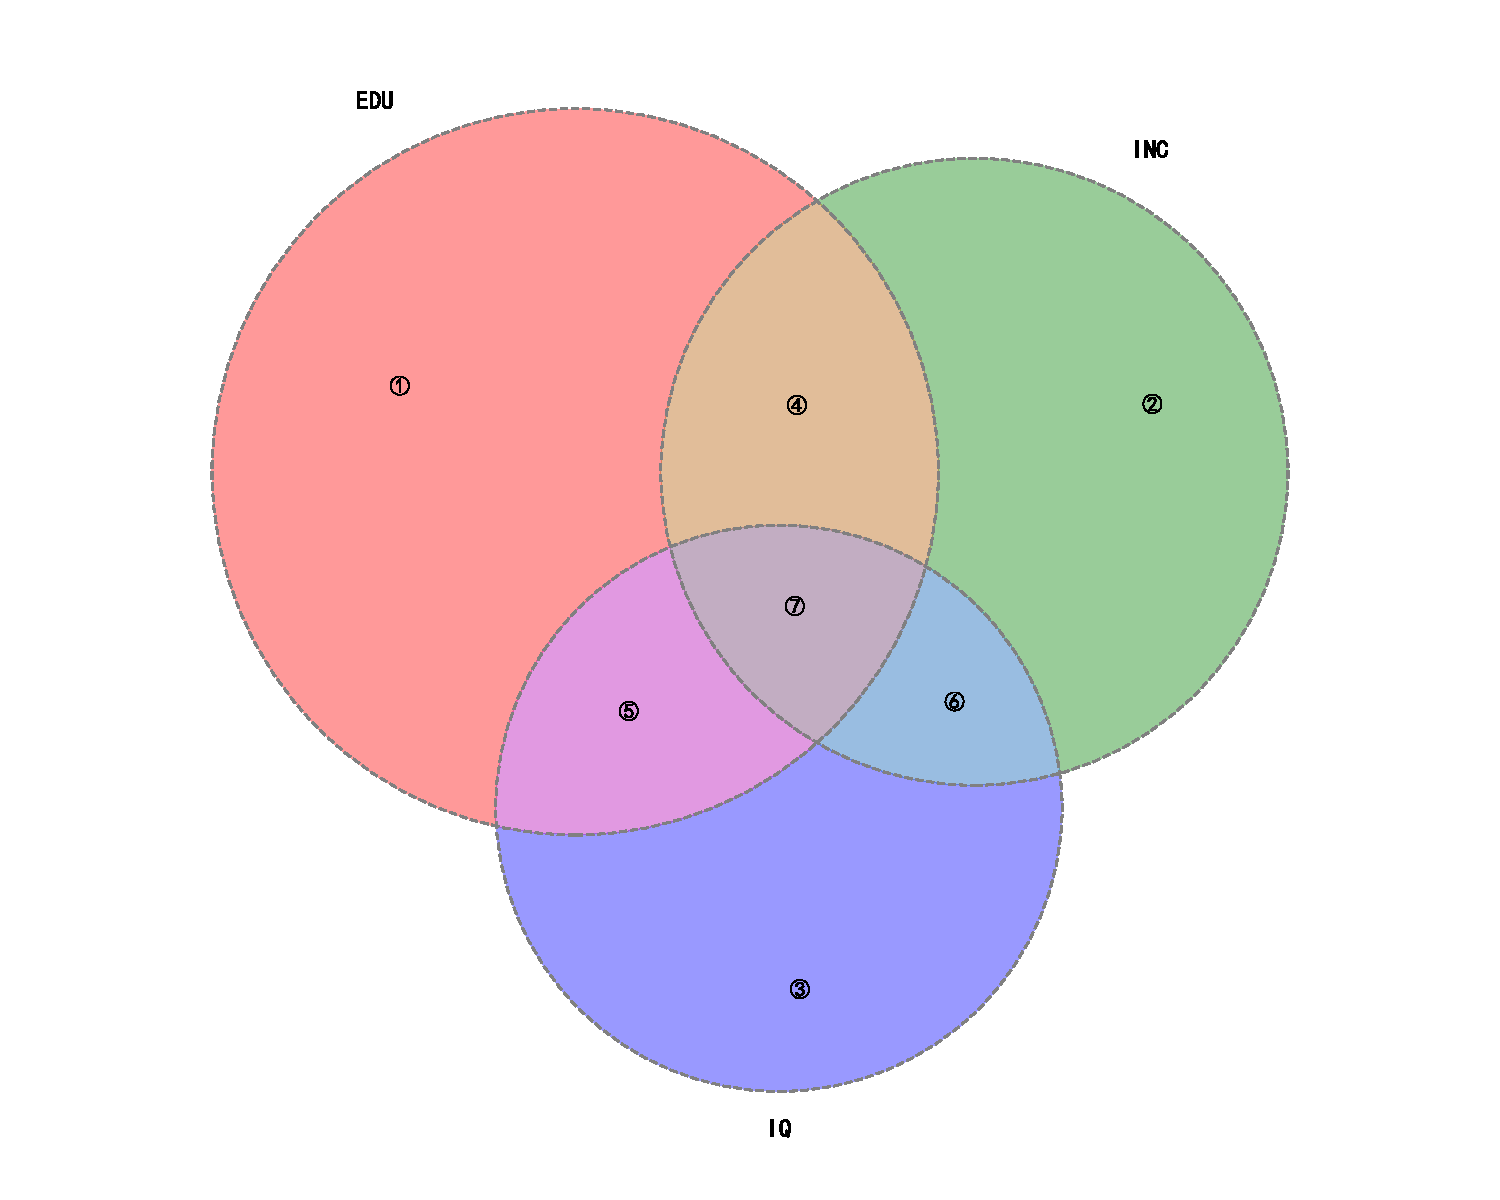
\includegraphics[width=0.5\textwidth]{image/venn_diagrams.pdf}}
	\caption{收入与教育间关系的韦恩图}
	\label{fig:venn}
\end{figure}

在这个图中,我们很清晰地看到,没有一个变量具有超凡脱俗的地位(也就是无法确定哪个是被解释变量,哪个是解释变量)。各个变量之间拥有一部分相互交叉的区域,这构成了其关联的部分,也即统计推断意图找到的参数。同时,还包括处于一些外在的区域,这一部分完全可以归入 $\varepsilon$ ——也就是外部的影响因素之中。

故而统计推断始终面临着的问题便是:\textbf{相关性不等于因果性。}但是,相关始终是因果的一个必要条件。依据惯习,从小样本开始学习较为合适。

\subsection{小样本OLS}

\paragraph*{三大假定}

\textbf{线性假定}
古典线性回归模型(Classical Linear Regression Model,CLRM)可以表示为:

\begin{equation}
Y_i = \beta_1 X_{i1} + \beta_2 X_{i2} + \ldots + \beta_K X_{iK} + \varepsilon_i \quad (i=1,\ldots,n)
\end{equation}

其中,$n$表示样本容量,$X_{ij}$代表第$i$个观测值的第$j$个解释变量($j = 1, \ldots, K$),而$\beta_1, \ldots, \beta_K$则是待估参数(回归系数)。特别地,若模型包含常数项,通常令$X_{i1}=1$。

线性假定的核心含义在于每个解释变量对被解释变量的边际效应为常数。值得注意的是,虽然称为"线性"假定,但模型中可以包含高次项或交互项来处理非线性关系,这仍然被视为满足线性假定。例如,一个模型可以表示为:

\begin{equation}
	Y_i = \beta_1 X_{i1} + \beta_2 X_{i1}^2 + \beta_3 X_{i1}^3 + \beta_4 X_{i2} + \beta_5 X_{i3} + \varepsilon_i \quad (i=1,\ldots,n)
\end{equation}

这是一个包含高次项的模型,其中$X_{i1}$的二次项$X_{i1}^2$和三次项$X_{i1}^3$被引入模型中。尽管模型中包含了变量的高次项,但该模型仍然是线性模型,因为模型关于参数$\beta_1, \beta_2, \ldots, \beta_{5}$是线性的。也就是说,每个参数都以一次方的形式出现,参数之间没有相乘或非线性关系。

在实际应用中,我们可以将$X_{i1}^2$看作一个新的变量$Z_{i1}=X_{i1}^2$,将$X_{i1}^3$看作另一个新变量$Z_{i2}=X_{i1}^3$,这样模型就转化为标准的线性形式:

\begin{equation}
	Y_i = \beta_1 X_{i1} + \beta_2 Z_{i1} + \beta_3 Z_{i2} + \cdots + \varepsilon_i \quad (i=1,\ldots,n)
\end{equation}

因此,只要模型关于参数是线性的,无论变量之间存在怎样的非线性关系,该模型都属于线性回归模型的范畴。

为了更简洁地表达模型,我们定义以下矩阵:
\begin{itemize}
\item $\mathbf{x}_i' = (X_{i1}, X_{i2}, \ldots, X_{iK})$
\item $\boldsymbol{\beta} = (\beta_1, \beta_2, \ldots, \beta_K)'$
\item $\varepsilon_i$表示扰动项
\end{itemize}

单个观测方程可以表示为:
\begin{equation}
Y_i = \mathbf{x}_i' \boldsymbol{\beta} + \varepsilon_i \quad (i=1,\ldots,n) 
\end{equation}

将所有观测方程叠放,我们得到:
\begin{equation}
\mathbf{Y} = \mathbf{X} \boldsymbol{\beta} + \boldsymbol{\varepsilon}
\end{equation}

其中:
\begin{itemize}
\item $\mathbf{Y} = (Y_1, Y_2, \ldots, Y_n)'$
\item $\mathbf{X} = (\mathbf{x}_1, \mathbf{x}_2, \ldots, \mathbf{x}_n)'$是$n \times K$的设计矩阵
\item $\boldsymbol{\varepsilon} = (\varepsilon_1, \varepsilon_2, \ldots, \varepsilon_n)'$是扰动项向量
\end{itemize}

\textbf{严格外生性假定}

严格外生性假定表示为:
\begin{equation}
E(\varepsilon_i | \mathbf{X}) = E(\varepsilon_i | \mathbf{x}_1, \ldots, \mathbf{x}_n) = 0 \quad (i=1,\ldots,n)
\end{equation}

这一假定的含义是,给定数据矩阵$\mathbf{X}$,扰动项的条件期望为零。这意味着$\varepsilon_i$均值独立于所有解释变量的观测数据。由此可以推导出两个重要推论:首先,扰动项的无条件期望也为零,即$E(\varepsilon_i) = 0$;其次,解释变量与扰动项正交,即$Cov(\mathbf{x}_{ik}, \varepsilon_i) = 0$。

如果严格外生性假定被违反,即$E(\varepsilon_i|\mathbf{X}) \neq 0$ 时,将会产生以下后果:

最小二乘估计(Ordinary Least Squares, OLS)将不再是无偏的(unbiased),其推论与统计性质将受到严重影响,主要后果包括:

\begin{enumerate}
\item OLS估计量偏误(Bias):
若扰动项与解释变量存在相关性,OLS估计的系数将系统性偏离真实值,即 $E(\hat{\boldsymbol{\beta}}) \neq \boldsymbol{\beta}$ 。这种偏误不是由样本波动引起的,而是源于模型设定中系统性的信息遗漏或内生性问题。

\item 估计量不再一致(Inconsistency):
在样本容量趋近无穷时,OLS估计也不能收敛于真实参数值,即不满足一致性(consistency)。这意味着收集更多的数据并不能解决偏误问题。

\item 回归结果不可解释为因果效应:
如果解释变量与误差项相关,回归系数不再具有因果解释,因为部分变异源于未被模型控制的系统性因素,因果推断的基础条件——可忽略性(ignorability)或条件独立性——遭到破坏。

\item 推论统计量失效:
OLS估计量的标准误可能低估或高估实际的不确定性,导致 $t$ 检验和 $F$ 检验的显著性水平失真,从而产生虚假显著或遗漏显著变量。
\end{enumerate}

\textbf{为何产生内生性问题(Endogeneity)?}

违反严格外生性假定通常是由于模型中存在遗漏变量(omitted variables)、互为因果(simultaneity)和测量误差(measurement error)等内生性来源,这些问题必须通过其他方法(如工具变量法、双重差分、固定效应模型等)加以处理。


因此,严格外生性是OLS估计可靠性的基石,一旦被违反,必须通过理论论证和实证检验识别偏误来源,并考虑替代的识别策略,这也是统计推断迈向因果推断的关键环节。

\textbf{不存在严格多重共线性假定}

该假定要求数据矩阵$\mathbf{X}$满列秩:
\begin{equation}
	\text{rank}(\mathbf{X}) = K
\end{equation}

如果这一条件不满足,则参数$\boldsymbol{\beta}$不可识别(有趣的案例可见第三章中对KKV三人理论的介绍)。在实际应用中,除非设置过多虚拟变量且包含常数项,否则严格多重共线性的情况较为少见。

满足上述三大假定可以帮助我们实现对方程整体的正确估计,但是,为了确保模型有效性,我们需要考虑残差性质。因而继续引入了更多假定:

\textbf{球型扰动项假定}

球型扰动项假定的矩阵形式为:
\begin{equation}
	Var(\boldsymbol{\varepsilon} | \mathbf{X}) = \sigma^2 \mathbf{I}_n
\end{equation}

其中:
\begin{equation*}
	\boldsymbol{\varepsilon} = 
	\begin{pmatrix}
	\varepsilon_1 \\
	\varepsilon_2 \\
	\vdots \\
	\varepsilon_n
	\end{pmatrix} \quad 
	\mathbf{I}_n = 
	\begin{pmatrix}
	1 & 0 & \cdots & 0 \\
	0 & 1 & \cdots & 0 \\
	\vdots & \vdots & \ddots & \vdots \\
	0 & 0 & \cdots & 1
	\end{pmatrix}
\end{equation*}

这表明误差项向量服从均值为0,协方差矩阵为 $\sigma^2 \mathbf{I}_n$ 的多元正态分布,其中每个误差项的方差都是 $\sigma^2$,且误差项之间互不相关。

这一假定包含两个重要性质:条件同方差性($Var(\varepsilon_i | \mathbf{X}) = \sigma^2$)和无自相关性($Cov(\varepsilon_i, \varepsilon_j | \mathbf{X}) = 0$对于$i \neq j$)。这些性质保证了OLS估计量的有效性,后续我们将考虑违背该假定下的情况以及如何修正。

\paragraph*{如何估计参数?}

回归模型建立之后,我们的首要任务是对模型中的参数进行估计。参数估计的方法主要包括最小二乘估计(Ordinary Least Squares, OLS)、最大似然估计(Maximum Likelihood Estimation, MLE)以及矩估计(Method of Moments)。本节将围绕最为基础且广泛使用的最小二乘估计展开介绍。

\textbf{残差平方和最小化}

在线性回归模型中,最小二乘法的核心思想是使残差平方和(Sum of Squared Residuals, SSR)最小。对于参数的任意假设值$\tilde{\boldsymbol{\beta}}$,我们定义残差向量为:
\begin{equation}
\mathbf{e} = \mathbf{Y} - \mathbf{X}\tilde{\boldsymbol{\beta}}
\end{equation}

最小化的目标函数为残差平方和:
\begin{equation}
	SSR(\tilde{\boldsymbol{\beta}}) = \sum_{i=1}^n e_i^2 = \mathbf{e}'\mathbf{e} = (\mathbf{Y} - \mathbf{X}\tilde{\boldsymbol{\beta}})'(\mathbf{Y} - \mathbf{X}\tilde{\boldsymbol{\beta}})
\end{equation}

展开上述表达式,可得:
\begin{equation}
	SSR(\tilde{\boldsymbol{\beta}}) = \mathbf{Y}'\mathbf{Y} - 2\mathbf{Y}'\mathbf{X}\tilde{\boldsymbol{\beta}} + \tilde{\boldsymbol{\beta}}'\mathbf{X}'\mathbf{X}\tilde{\boldsymbol{\beta}}
\end{equation}

\begin{tcolorbox}[title=使用Stata 中的 auto 数据集进行演示, colback=white, colframe=black, colbacktitle=white, coltitle=black,fonttitle=\bfseries]
	\begin{lstlisting}[xleftmargin=2em, commentstyle=\color{black}]
clear all
quietly sysuse auto, clear

* 我们设定一个简单的小样本回归模型(含截距)
* 以 price 为因变量,mpg, weight, foreign 为解释变量
regress price mpg weight foreign
	\end{lstlisting}
	\vspace{-2em}
	\begin{Verbatim}[commandchars=\\\{\},xleftmargin=2em]

      Source |       SS           df       MS      Number of obs   =        74
-------------+----------------------------------   F(3, 70)        =     23.29
       Model |   317252881         3   105750960   Prob > F        =    0.0000
    Residual |   317812515        70  4540178.78   R-squared       =    0.4996
-------------+----------------------------------   Adj R-squared   =    0.4781
       Total |   635065396        73  8699525.97   Root MSE        =    2130.8

------------------------------------------------------------------------------
       price | Coefficient  Std. err.      t    P>|t|     [95\% conf. interval]
-------------+----------------------------------------------------------------
         mpg |    21.8536   74.22114     0.29   0.769    -126.1758     169.883
      weight |   3.464706    .630749     5.49   0.000     2.206717    4.722695
     foreign |    3673.06   683.9783     5.37   0.000     2308.909    5037.212
       \_cons |  -5853.696   3376.987    -1.73   0.087    -12588.88    881.4934
------------------------------------------------------------------------------
	\end{Verbatim}

\end{tcolorbox}

\textbf{向量微分与正规方程}

利用向量微分规则,对$SSR(\tilde{\boldsymbol{\beta}})$关于$\tilde{\boldsymbol{\beta}}$求导,并令导数为零,即可得到最小值的条件:
\begin{equation}
	\frac{\partial SSR}{\partial \tilde{\boldsymbol{\beta}}} = -2\mathbf{X}'\mathbf{Y} + 2\mathbf{X}'\mathbf{X}\tilde{\boldsymbol{\beta}} = \mathbf{0}
\end{equation}

这便是所谓的正规方程(Normal Equation):
\begin{equation}
	\mathbf{X}'\mathbf{X}\hat{\boldsymbol{\beta}} = \mathbf{X}'\mathbf{Y}
\end{equation}

在$\mathbf{X}'\mathbf{X}$是可逆的前提下(也就是不存在严格的多重共线问题),我们可以求得最小二乘估计量:
\begin{equation}
	\hat{\boldsymbol{\beta}} = (\mathbf{X}'\mathbf{X})^{-1}\mathbf{X}'\mathbf{Y}
\end{equation}

\begin{tcolorbox}[title=在 Stata 的 Mata 中用矩阵(正规方程)显式计算 OLS 解, colback=white, colframe=black, colbacktitle=white, coltitle=black,fonttitle=\bfseries]
	\begin{lstlisting}[xleftmargin=2em, commentstyle=\color{black}]
* 构造设计矩阵 X 与因变量向量 Y(排除缺失)
quietly keep if !missing(price, mpg, weight, foreign)

* 生成常数项并保存数据顺序索引
capture gen double cons = 1
quietly order cons price mpg weight foreign

* 创建 X 矩阵与 Y 向量到 Mata,做矩阵运算
mata:
st_view(Y=., ., "price") // 创建一个指向变量price的视图矩阵Y
st_view(X=., ., ("cons","mpg","weight","foreign")) // 创建指向变量的视图矩阵X
/* 计算 OLS */
b = invsym(X'*X) * (X'*Y)  // 使用正规方程计算OLS估计量:b = (X'X)^(-1)X'Y
b = colshape(b, 1) // 确保b是列向量形式
st_numscalar("n_obs", rows(X)) // 将观测数(X的行数)存储为标量n_obs
b // 显示计算得到的系数向量b
end

* 把 Mata 得到的系数显示与 regress 对比
matrix list e(b)       // 来自 regress 的系数(行向量)
mata: st_matrix("b_mata", b')   // 转成 Stata 矩阵形式(1 x K)
matrix list b_mata
	\end{lstlisting}
	\vspace{-2em}
	\begin{Verbatim}[commandchars=\\\{\},xleftmargin=2em]

. mata:
…… 过程省略
: end

e(b)[1,4]
           mpg      weight     foreign       \_cons
y1   21.853604   3.4647058   3673.0604  -5853.6957

b\_mata[1,4]
            c1          c2          c3          c4
r1   21.853604   3.4647058   3673.0604  -5853.6957
	\end{Verbatim}

\end{tcolorbox}

\textbf{残差性质与方差估计}

估计得出参数后,我们可以计算残差向量$\hat{\mathbf{e}} = \mathbf{Y} - \mathbf{X}\hat{\boldsymbol{\beta}}$。这一残差向量具有与解释变量正交的重要性质,即:
\begin{equation}
\mathbf{X}'\hat{\mathbf{e}} = \mathbf{0}
\end{equation}

这意味着,拟合值$\hat{\mathbf{Y}} = \mathbf{X}\hat{\boldsymbol{\beta}}$与残差$\hat{\mathbf{e}}$在向量空间中正交,两者共同构成了$\mathbf{Y}$的正交分解。

进一步地,我们可以得到误差项方差$\sigma^2$的无偏估计量:
\begin{equation}
	s^2 = \frac{1}{n-K} \sum_{i=1}^n \hat{e}_i^2 = \frac{\hat{\mathbf{e}}'\hat{\mathbf{e}}}{n-K}
\end{equation}

其中$n-K$为自由度,$K$为解释变量(含截距项)个数。标准误差定义为$s = \sqrt{s^2}$,它衡量了残差的离散程度。

\begin{tcolorbox}[title=在 Stata 的 Mata 中计算残差、SSR、$s^2$ 与协方差矩阵、标准误, colback=white, colframe=black, colbacktitle=white, coltitle=black,fonttitle=\bfseries]
	\begin{lstlisting}[xleftmargin=2em, commentstyle=\color{black}]
mata:
/* 重新读取 X,Y,b */
st_view(Y=., ., "price") // 创建指向因变量price的视图矩阵Y
st_view(X=., ., ("mpg","weight","foreign","cons")) // 创建指向自变量的视图矩阵X
b = invsym(X'*X) * (X'*Y) // 使用正规方程计算OLS估计量:b = (X'X)^(-1)X'Y
Yhat = X * b // 计算拟合值:Yhat = X*b
e = Y - Yhat // 计算残差向量:e = Y - Yhat
RSS = e'*e // 计算残差平方和:RSS = e'*e
n = rows(X) // 获取样本数量(观测数)
K = cols(X) // 获取参数个数(变量个数)
s2 = RSS / (n - K) // 计算误差项方差的无偏估计:s² = RSS/(n-K)
s = sqrt(s2) // 计算残差标准差:s = √s²
Vb = s2 * invsym(X'*X) // 计算参数估计量的协方差矩阵:Var(b) = s²(X'X)^(-1)
se = sqrt(diagonal(Vb)) // 提取协方差矩阵对角线元素的平方根得到标准误
/* 输出 */
st_numscalar("RSS", RSS[1,1]) // 将RSS存储为Stata标量
st_numscalar("s2", s2[1,1]) // 将s²存储为Stata标量
st_numscalar("s", s[1,1]) // 将s存储为Stata标量
st_matrix("Vb", Vb) // 将协方差矩阵Vb存储为Stata矩阵
st_matrix("se_b", se') // 将标准误向量存储为Stata矩阵
st_matrix("b_hat", b') // 将参数估计值存储为Stata矩阵
end

display "残差平方和 RSS = " %9.4f RSS
display "误差方差的无偏估计 s^2 = " %9.6f s2
display "残差标准差 s = " %9.6f s
matrix list Vb
matrix list se_b
matrix list b_hat

* 比较 Stata 的 e(V) 与 我们计算的 Vb
matrix list e(V)
* e(V) 和 Vb 数值相同
	\end{lstlisting}

\end{tcolorbox}
\begin{tcolorbox}[title=在 Stata 的 Mata 中计算残差、SSR、$s^2$ 与协方差矩阵、标准误, colback=white, colframe=black, colbacktitle=white, coltitle=black,fonttitle=\bfseries]
	\vspace{-2em}

	\begin{Verbatim}[commandchars=\\\{\},xleftmargin=2em]


. mata:
…… 过程省略
: end

残差平方和 RSS =  3.18e+08
误差方差的无偏估计 s\^{}2 =  4.54e+06
残差标准差 s =  2.13e+03

symmetric Vb[4,4]
            c1          c2          c3          c4
r1   5508.7774
r2     36.2912   .39784425
r3   9089.6431     218.835   467826.27
r4   -229604.2  -2039.2381  -993431.72    11404044

se\_b[1,4]
           c1         c2         c3         c4
r1  74.221139  .63074896  683.97827  3376.9874

b\_hat[1,4]
            c1          c2          c3          c4
r1   21.853604   3.4647058   3673.0604  -5853.6957

symmetric e(V)[4,4]
                mpg      weight     foreign       \_cons
    mpg   5508.7774
 weight     36.2912   .39784425
foreign   9089.6431     218.835   467826.27
  \_cons   -229604.2  -2039.2381  -993431.72    11404044
	\end{Verbatim}

\end{tcolorbox}

\begin{tcolorbox}[title=在 Stata 的 Mata 中验证(残差与解释变量正交), colback=white, colframe=black, colbacktitle=white, coltitle=black, fonttitle=\bfseries]
	\begin{lstlisting}[xleftmargin=2em, commentstyle=\color{black}]
* 先生成常数项
capture gen double cons = 1

* 先预测残差
predict double ehat, resid

* 在 Mata 中读取 X 和 ehat,并计算 X'e
mata:
st_view(X=., ., ("cons","mpg","weight","foreign"))
st_view(e=., ., "ehat")
Xe = X' * e
Xe
end
display "理论上 X' * e = 0,各项应接近 0"
	\end{lstlisting}
	\vspace{-2em}
	\begin{Verbatim}[commandchars=\\\{\},xleftmargin=2em]

. mata:
------------------------------------------------- mata (type end to exit) -----
: st\_view(X=., ., ("cons","mpg","weight","foreign"))
: st\_view(e=., ., "ehat")
: Xe = X' * e
: Xe
                 1
    +---------------+
  1 |  1.16415e-10  |
  2 |  2.11003e-09  |
  3 |  3.42727e-07  |
  4 |  3.63798e-12  |
    +---------------+
: end
-------------------------------------------------------------------------------
理论上 X' * e = 0,各项应接近 0
	\end{Verbatim}

\end{tcolorbox}

\textbf{Frisch--Waugh--Lovell(FWL)定理}

FWL 定理揭示了多元回归中某个变量系数的估计,可以通过“残差回归”的方式得到。设我们有如下的多元线性回归模型:
\begin{equation}
\mathbf{Y} = \mathbf{X}_1 \beta_1 + \mathbf{X}_2 \beta_2 + \boldsymbol{\varepsilon}
\end{equation}

其中 $\mathbf{Y}$ 为 $n \times 1$ 因变量向量,$\mathbf{X}_1$ 为 $n \times k_1$ 的解释变量矩阵,$\mathbf{X}_2$ 为 $n \times k_2$ 的控制变量矩阵。

在多元回归中,$\beta_1$ 衡量的是在控制了 $X_2$ 的影响后,$X_1$ 对 $Y$ 的边际效应。FWL 定理告诉我们,我们可以在不直接进行多元回归的情况下,通过对变量进行“净化”(消去 $X_2$ 的部分)来得到同样的系数估计。

假设我们仅关心 $\beta_1$ 的估计值,可以按以下三步操作:
\begin{enumerate}
	\item 将 $Y$ 对 $X_2$ 回归,取残差 $e_Y$,即
	\begin{equation}
	e_Y = Y - \hat{\alpha}_0 - \hat{\alpha}_2 X_2
	\end{equation}

	\item 将 $X_1$ 对 $X_2$ 回归,取残差 $e_{X_1}$,即
	\begin{equation}
	e_{X_1} = X_1 - \hat{\gamma}_0 - \hat{\gamma}_2 X_2
	\end{equation}

	\item 将 $e_Y$ 对 $e_{X_1}$ 进行一元回归,得到的回归系数即为 $\beta_1$ 的估计值:
	\begin{equation}
	e_Y = \beta_1 e_{X_1} + \text{residual}
	\end{equation}
\end{enumerate}

这种方法的实质是:先用 $X_2$ 消除 $Y$ 与 $X_1$ 中由 $X_2$ 解释的部分,然后在“净化”后的数据之间建立回归关系。

FWL 定理的矩阵证明,$\beta_1$ 的 OLS 估计可以通过如下步骤获得:

\begin{enumerate}
	\item \textbf{对 $\mathbf{Y}$ 回归 $\mathbf{X}_2$,取残差:}
	\begin{equation}
	\mathbf{e}_Y = \mathbf{M}_2 \mathbf{Y}
	\end{equation}

	其中 $\mathbf{M}_2 = \mathbf{I} - \mathbf{P}_2$,$\mathbf{P}_2 = \mathbf{X}_2(\mathbf{X}_2'\mathbf{X}_2)^{-1}\mathbf{X}_2'$ ,其是 $\mathbf{X}_2$ 的投影矩阵。
	\item \textbf{对 $\mathbf{X}_1$ 的每一列回归 $\mathbf{X}_2$,取残差:}
	\begin{equation}
	\mathbf{e}_{X_1} = \mathbf{M}_2 \mathbf{X}_1
	\end{equation}
	
	即对 $\mathbf{X}_1$ 的每一列都做一次“净化”。
	\item \textbf{用 $\mathbf{e}_Y$ 对 $\mathbf{e}_{X_1}$ 做一元或多元回归,得到系数:}
	\begin{equation}
	\hat{\beta}_1 = \left( \mathbf{X}_1'\mathbf{M}_2\mathbf{X}_1 \right)^{-1} \mathbf{X}_1'\mathbf{M}_2\mathbf{Y}
	\end{equation}

	这与直接对 $\mathbf{Y}$ 回归 $\mathbf{X}_1$ 和 $\mathbf{X}_2$ 得到的 $\beta_1$ 完全一致。
\end{enumerate}

$\mathbf{M}_2$ 的作用是将向量投影到与 $\mathbf{X}_2$ 张成空间正交的子空间,即“剔除”了 $\mathbf{X}_2$ 的影响。FWL 定理说明,控制变量的作用就是把因变量和解释变量都净化后再做回归,得到的系数就是多元回归中该变量的边际效应。

FWL 定理的重要意义在于,它为多元回归系数提供了一个分解式解释:\textbf{多元回归中的某个系数等于“净化”该变量与因变量后,两者之间的一元回归系数}。这一结果不仅在理论推导中有用,更为理解控制变量的本质提供了数理上的直观视角。

在韦恩图\ref{fig:venn}中:
\begin{itemize}
    \item INC 与 IQ 的重叠部分⑥⑦表示 IQ 对收入的解释部分;
    \item EDU 与 IQ 的重叠部分⑤⑦表示 IQ 对教育的解释部分。
\end{itemize}

我们通过第一步和第二步回归,分别剔除了 INC 和 EDU 中由 IQ 解释的那一部分(即图中 IQ 与其他圆的重叠部分⑤⑥⑦)

第三步回归实质上是在比较两个“去掉 IQ 影响后的残差”之间的关系,即对应于图中 EDU 与 INC 在 IQ 之外的交集区域(也就是④)。

\begin{tcolorbox}[title=在 Stata 中展示FWL定理, colback=white, colframe=black, colbacktitle=white, coltitle=black,fonttitle=\bfseries]
	\begin{lstlisting}[xleftmargin=2em, commentstyle=\color{black}]
* 目标:展示在控制 weight, foreign 时 mpg 的系数
* 等同于:先对 price 与 mpg 分别“剔除” weight & foreign 的影响,再做一元回归
* 先看完整模型中 mpg 的估计系数(已在 regress 输出)
quietly regress price mpg weight foreign
local b1 = _b[mpg]
display "多元回归中 mpg 的系数 = " %9.6f `b1'
* 第一步:price 对 weight foreign 回归,取残差 eY
quietly regress price weight foreign
capture predict double eY, resid
* 第二步:mpg 对 weight foreign 回归,取残差 eX1
quietly regress mpg weight foreign
capture predict double eX1, resid
* 第三步:用 eY 对 eX1 做一元回归
quietly regress eY eX1
local b2 = _b[eX1]
display "用 eY 对 eX1 做一元回归得到的系数 = " %9.6f `b2'
* 第四步:进一步讨论 FWL 定理
quietly regress price eX1
local b3 = _b[eX1]
display "用 Y 对 eX1 做一元回归得到得到的系数 = " %9.6f `b3'
* 第五步:进一步讨论 FWL 定理
quietly regress eY mpg weight foreign
local b4 = _b[mpg]
display "用 eY 对 mpg 做多元回归得到得到的系数 = " %9.6f `b4'
	\end{lstlisting}
	\vspace{-2em}
	\begin{Verbatim}[commandchars=\\\{\},xleftmargin=2em]

多元回归中 mpg 的系数 = 21.853604
用 eY 对 eX1 做一元回归得到的系数 = 21.853604
用 Y 对 eX1 做一元回归得到得到的系数 = 21.853604
用 eY 对 mpg 做多元回归得到得到的系数 = 21.853604
	\end{Verbatim}

\end{tcolorbox}

图\ref{fig:venncol}表示的是一个高度共线情况下的韦恩图,从图中我们可以看到,IQ 与 INC 的重叠部分⑥⑦表示 IQ 对收入的解释部分;IQ 与 EDU 的重叠部分⑤⑦表示 IQ 对教育的解释部分。在剔除IQ影响后的残差之间进行一元回归,得到的回归系数即为 EDU 的估计值,但是由于这一部分过于庞大,因此我们无法从结果中得到有效的解释。

\begin{figure}[ht]
	\centering
	\fbox{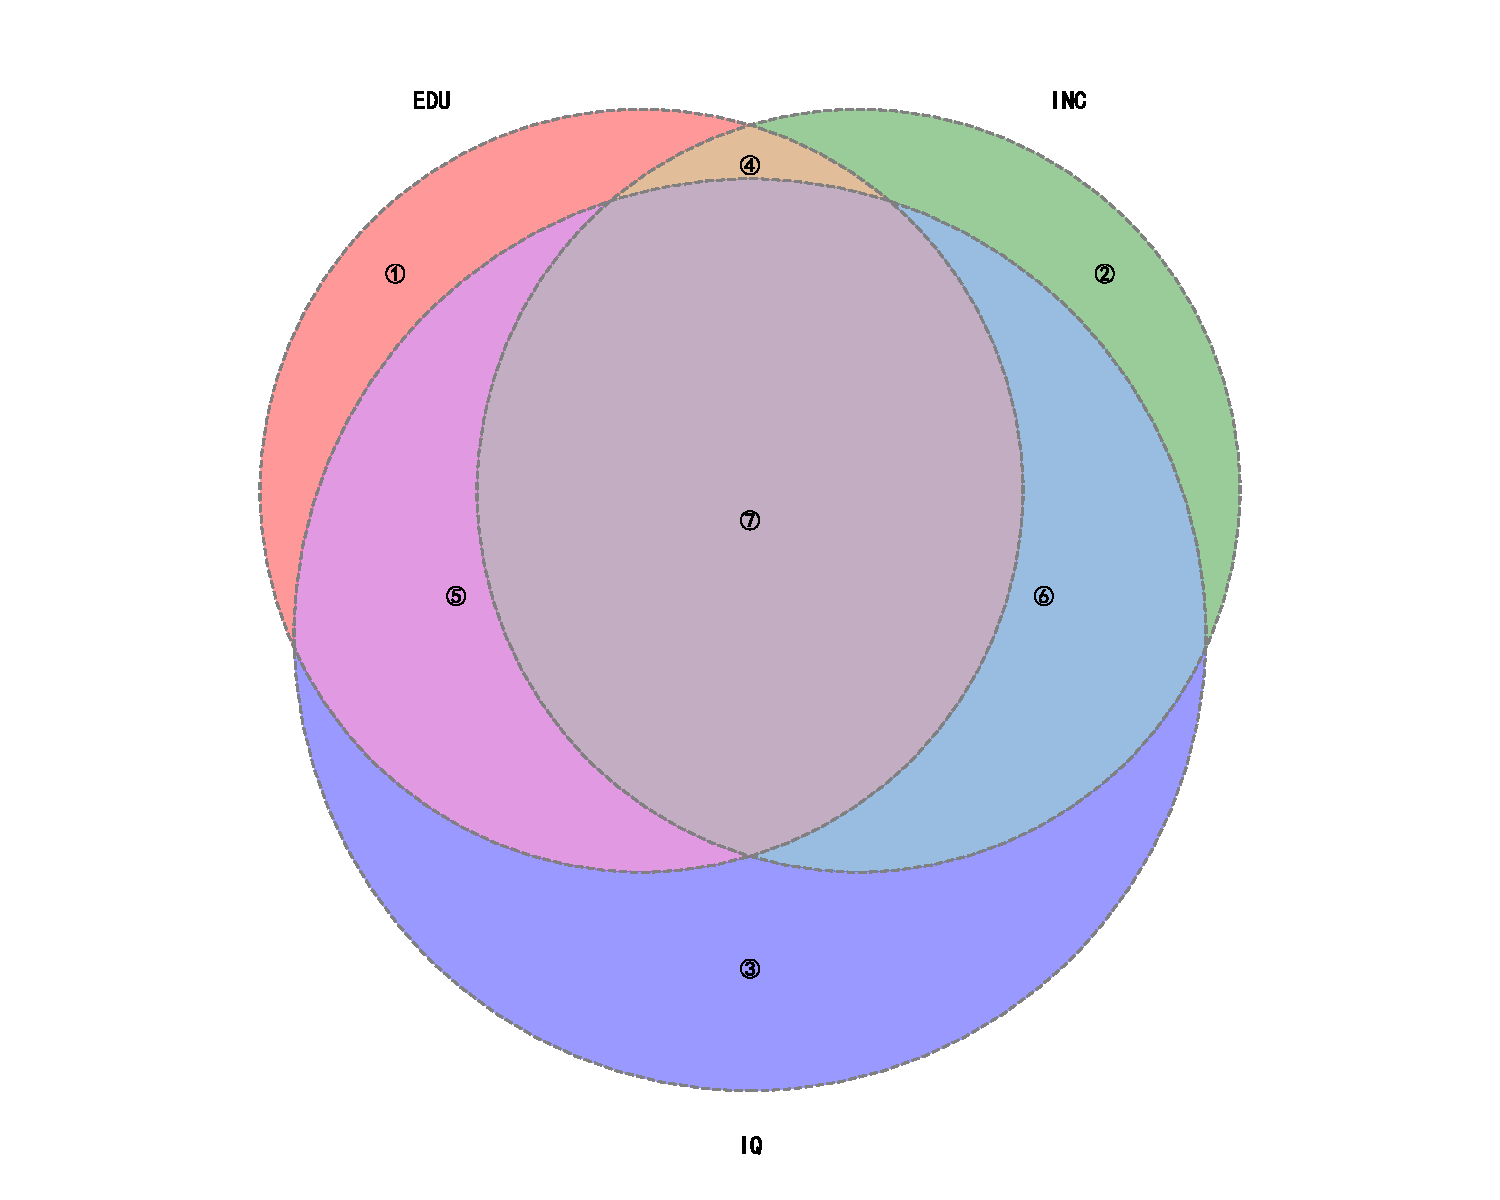
\includegraphics[width=0.5\textwidth]{image/venn_diagrams_collinearity.pdf}}
	\caption{高度共线下的韦恩图}
	\label{fig:venncol}
\end{figure}

\newpage

\textbf{平方和分解与拟合优度}

若模型中包含常数项,我们可以建立响应变量的平方和分解:
\begin{equation}
	\sum_{i=1}^n (Y_i - \bar{Y})^2 = \sum_{i=1}^n (\hat{Y}_i - \bar{Y})^2 + \sum_{i=1}^n \hat{e}_i^2
\end{equation}

其中,左侧为总离差平方和(Total Sum of Squares, TSS),右侧第一项为回归平方和(Explained Sum of Squares, ESS),第二项为残差平方和(Residual Sum of Squares, RSS)。据此定义拟合优度$R^2$为:
\begin{equation}
	R^2 = \frac{ESS}{TSS} = 1 - \frac{RSS}{TSS}
\end{equation}

该指标反映了模型解释总变异的能力,其数值介于0与1之间,越接近1表示模型拟合越好。该指标在多数统计软件中会自动给出,用以反映无截距模型的拟合程度。

通俗地说,我们可以将总变异(TSS)理解为数据的"总信息量",它被分解为两部分:
\begin{itemize}
\item 由模型解释的部分(ESS):这是我们通过自变量能够捕捉到的"有用信息"
\item 未被模型解释的部分(RSS):这是模型无法解释的"剩余信息"或"噪音"
\end{itemize}

$R^2$就像一个"信息利用率"指标,告诉我们模型能够解释多少比例的数据变异。例如,$R^2=0.5$意味着模型能够解释因变量中50\%的变异。

需要注意的是,简单地增加变量数量通常会使$R^2$增大,但这并不意味着模型质量提高。为了惩罚变量过多可能导致的虚高$R^2$,我们引入校正拟合优度$\bar{R}^2$(Adjusted $R^2$),校正后的$R^2$考虑了模型复杂度,只有当新增变量带来的信息增益超过其增加的复杂度时,$\bar{R}^2$才会增加:

\begin{equation}
	\bar{R}^2 = 1 - \frac{RSS/(n-K)}{TSS/(n-1)} = 1 - \frac{n-1}{n-K}(1-R^2)
\end{equation}

在\textbf{机器学习(ML)}中,$R^2$ 往往被视为预测精度的重要度量之一,其优化目标是尽可能减少预测误差。然而在因果推断中,研究者的核心关注点并非预测准确,而是获得对处理效应(treatment effect)的无偏、可解释估计值。一个因果模型即便 $R^2$ 较低,只要能够正确识别出因果效应,也具有高度学术价值;反之,一个 $R^2$ 极高但因果识别错误的模型,在政策建议或理论解释上可能毫无意义,故而社会科学范式中对于 $R^2$ 的考量往往并不严格。

\begin{tcolorbox}[title={在 Stata 的 Mata 中进行平方和分解($TSS = ESS + RSS$)与 $R^2$ 计算}, colback=white, colframe=black, colbacktitle=white, coltitle=black, fonttitle=\bfseries]
	\begin{lstlisting}[xleftmargin=2em, commentstyle=\color{black}]
* 计算 TSS, ESS, RSS 并核对 R^2
summarize price, meanonly // 计算price变量的均值
scalar Ybar = r(mean) // 将price的均值存储为标量Ybar
quietly regress price mpg weight foreign // 静默运行回归(不显示结果)
scalar b_cons = _b[_cons] // 提取并存储常数项系数
scalar b_mpg = _b[mpg] // 提取并存储mpg变量的系数
scalar b_weight = _b[weight] // 提取并存储weight变量的系数
scalar b_foreign = _b[foreign] // 提取并存储foreign变量的系数
capture generate double Yhat = b_cons + b_mpg*mpg + b_weight*weight + b_foreign*foreign
// 根据系数计算拟合值Yhat
capture generate double resid = price - Yhat // 计算残差值(实际值减去拟合值)
quietly summarize price, detail // 静默计算price的详细统计信息

mata:
st_view(Y=., ., "price") // 创建指向price变量的视图矩阵Y
st_view(Yhat=., ., "Yhat") // 创建指向Yhat变量的视图矩阵Yhat
st_view(resid=., ., "resid") // 创建指向resid变量的视图矩阵resid
TSS = (Y :- mean(Y))' * (Y :- mean(Y)) // 计算总离差平方和TSS = Σ(yi - ȳ)²
ESS = (Yhat :- mean(Y))' * (Yhat :- mean(Y)) // 计算回归平方和ESS = Σ(ŷi - ȳ)²
RSS = resid' * resid // 计算残差平方和RSS = Σ(êi)²
st_numscalar("TSS_s", TSS[1,1]) // 将TSS存储为Stata标量
st_numscalar("ESS_s", ESS[1,1]) // 将ESS存储为Stata标量
st_numscalar("RSS_s", RSS[1,1]) // 将RSS存储为Stata标量
end

display "TSS = " %9.4f scalar(TSS_s)
display "ESS = " %9.4f scalar(ESS_s)
display "RSS = " %9.4f scalar(RSS_s)
display "TSS - ESS - RSS = " %9.8f (scalar(TSS_s) - scalar(ESS_s) - scalar(RSS_s))
display "R^2 = " %9.6f (scalar(ESS_s) / scalar(TSS_s))
	\end{lstlisting}
	\vspace{-2em}
	\begin{Verbatim}[commandchars=\\\{\},xleftmargin=2em]

. mata:
…… 过程省略
: end
TSS =  6.35e+08
ESS =  3.17e+08
RSS =  3.18e+08
TSS - ESS - RSS = -0.00000036
R\^{}2 =  0.499559
	\end{Verbatim}

\end{tcolorbox}

\paragraph*{小样本下OLS估计的基本性质}
小样本下的OLS性质主要包括以下几个方面:

\textbf{线性}
    
    OLS估计量是被解释变量$\mathbf{y}$的线性组合:
    \begin{equation}
        \mathbf{b} = (\mathbf{X}^{\prime}\mathbf{X})^{-1}\mathbf{X}^{\prime}\mathbf{y}
    \end{equation}

\textbf{无偏性}
    
    在古典线性回归模型(CLRM)的假定下(严格外生性、无多重共线性、球型扰动项),OLS估计量是无偏的:
    \begin{equation}
        \operatorname{E}(\mathbf{b} \mid \mathbf{X}) = \boldsymbol{\beta}
    \end{equation}
    即$\mathbf{b}$不会系统性地高估或低估真实参数$\boldsymbol{\beta}$。无偏性的证明依赖于严格外生性假定:
    \begin{equation}
        \operatorname{E}(\epsilon_i \mid \mathbf{X}) = 0
    \end{equation}

\textbf{有效性(高斯-马尔可夫定理)}
    
    在CLRM假定下,OLS估计量是所有线性无偏估计量中方差最小的(BLUE)。即对于任意其他线性无偏估计量$\tilde{\boldsymbol{\beta}}$,有:
    \begin{equation}
        \operatorname{Var}(\tilde{\boldsymbol{\beta}} \mid \mathbf{X}) \geq \operatorname{Var}(\mathbf{b} \mid \mathbf{X})
    \end{equation}

\textbf{正态性与统计检验}
    
    若进一步假设扰动项$\epsilon_i$服从正态分布,则:
    \begin{itemize}
        \item OLS估计量$\mathbf{b}$服从多元正态分布。
        \item 对单个系数的$t$检验和对线性假设的$F$检验在小样本下严格成立(见后文)。
    \end{itemize}

\textbf{局限性}
    \begin{itemize}
        \item 严格外生性:要求解释变量与所有扰动项(过去、现在、未来)均不相关,时间序列中可能不成立。
        \item 正态性假设:若扰动项非正态,小样本下$t/F$检验可能失效,需依赖大样本理论。
        \item 异方差或自相关:若球型扰动项假定不成立,OLS虽无偏但不再有效,需使用GLS或稳健标准误。
    \end{itemize}

小样本下,OLS在CLRM假定下具有无偏性、有效性和正态性,是统计推断的基础。但实际应用中需谨慎检验假定(如异方差、自相关、内生性),必要时转向大样本理论或替代估计方法(如工具变量、GMM)。

\paragraph*{模型检验与预测}

在获得参数估计值之后,我们通常还需对模型的显著性进行检验,并评估模型在未来观测上的预测能力。本节将围绕线性回归模型中的方差估计、假设检验和预测方法进行介绍。

\textbf{方差估计}

如前所述,$s^2$是误差项方差$\sigma^2$的无偏估计量。这一结论基于矩阵迹(trace)运算的性质,具体地:
\begin{equation}
	E(\hat{\mathbf{e}}'\hat{\mathbf{e}} \mid \mathbf{X}) = \sigma^2 \cdot \text{trace}(\mathbf{M}) = \sigma^2 (n - K)
\end{equation}

因此,我们可得参数估计量$\hat{\boldsymbol{\beta}}$的协方差矩阵估计为:
\begin{equation}
	\widehat{\text{Var}}(\hat{\boldsymbol{\beta}} \mid \mathbf{X}) = s^2 (\mathbf{X}'\mathbf{X})^{-1}
\end{equation}

该协方差矩阵为后续进行假设检验和置信区间构建提供了基础。

\textbf{单个系数的检验}

在经典回归模型中,若我们进一步假定扰动项服从正态分布,即$\boldsymbol{\varepsilon} \sim \mathcal{N}(0, \sigma^2 \mathbf{I}_n)$,则参数估计量$\hat{\boldsymbol{\beta}}$亦服从正态分布。

此时,可对任一系数$\beta_k$构造t统计量进行假设检验:
\begin{equation}
	t_k = \frac{\hat{\beta}_k - \beta_k^0}{SE(\hat{\beta}_k)} \sim t(n-K)
\end{equation}

其中$\beta_k^0$为原假设下的理论值,$SE(\hat{\beta}_k)$为对应系数的标准误。我们可以通过计算$t_k$的值,并查阅$t$分布临界值或计算$p$值,判断该系数是否显著不同于零。

此外,置信区间的构建亦基于$t$分布,例如$(1-\alpha)$置信区间为:
\begin{equation}
\hat{\beta}_k \pm t_{\alpha/2}(n-K) \cdot SE(\hat{\beta}_k)
\end{equation}

通俗地说,t分布帮助我们判断回归系数的显著性。t统计量实际上是"信号"与"噪声"的比值:
\begin{itemize}
\item 分子$\hat{\beta}_k - \beta_k^0$代表我们观察到的"信号"(即实际效应与假设值的差异)
\item 分母$SE(\hat{\beta}_k)$代表"噪声"(即估计的不确定性)
\end{itemize}

当t值较大时,说明信号远大于噪声,我们更有信心认为该系数显著不为零。当样本量较小时,t分布比正态分布更"厚尾",能更好地反映小样本的不确定性。

\begin{tcolorbox}[title=在 Stata 的 Mata 中进行单个系数 t 检验, colback=white, colframe=black, colbacktitle=white, coltitle=black,fonttitle=\bfseries]
	\begin{lstlisting}[xleftmargin=2em, commentstyle=\color{black}]
* 检验 mpg 的显著性
* t_k = (b_k - 0) / se(b_k)
matrix list se_b // 列出之前计算的标准误矩阵se_b
mata:
b = st_matrix("b_mata")' // 从Stata矩阵中读取系数估计值,1xK转置为Kx1列向量
se = st_matrix("se_b")' // 从Stata矩阵中读取标准误,1xK转置为Kx1列向量
// 找到 mpg 在第2个位置 (mpg, weight, foreign, cons)
b_mpg = b[1] // 提取mpg变量的系数估计值(第1个位置)
se_mpg = se[1] // 提取mpg变量的标准误(第1个位置)
n = st_numscalar("n_obs") // 从Stata标量中读取样本数量n
K = 4 // 设置参数个数K=4
df = n - K // 计算自由度df = n - K
t_mpg = (b_mpg - 0) / se_mpg // 计算mpg系数的t统计量(原假设为0)
pval = 2 * ttail(df, abs(t_mpg)) // 计算双侧检验的p值(使用t分布的尾部概率)
st_numscalar("t_mpg", t_mpg) // 将计算得到的t统计量存储为Stata标量
st_numscalar("p_mpg", pval) // 将计算得到的p值存储为Stata标量
end

display "t = " %9.4f t_mpg ", p-value = " %9.6f p_mpg " (df = " (n_obs - 4) ")"
	\end{lstlisting}
	\vspace{-2em}
	\begin{Verbatim}[commandchars=\\\{\},xleftmargin=2em]

b\_mata[1,4]
            c1          c2          c3          c4
r1   21.853604   3.4647058   3673.0604  -5853.6957

se\_b[1,4]
           c1         c2         c3         c4
r1  74.221139  .63074896  683.97827  3376.9874

. mata:
…… 过程省略
: end

t =    0.2944, p-value =  0.769294 (df = 70)
	\end{Verbatim}

\end{tcolorbox}

\textbf{线性假设的检验}

当我们希望同时检验多个参数是否满足一组线性约束关系时,可以使用F检验方法。设原假设为:
\begin{equation}
H_0: \mathbf{R}\boldsymbol{\beta} = \mathbf{r}
\end{equation}

其中$\mathbf{R}$为$m \times K$的约束矩阵,$\mathbf{r}$为$m \times 1$的向量。

对应的F统计量为:
\begin{equation}
	F = \frac{(\mathbf{R}\hat{\boldsymbol{\beta}} - \mathbf{r})'[\mathbf{R}(\mathbf{X}'\mathbf{X})^{-1}\mathbf{R}']^{-1}(\mathbf{R}\hat{\boldsymbol{\beta}} - \mathbf{r}) / m}{s^2} \sim F(m, n - K)
\end{equation}

此统计量衡量在给定约束下估计结果偏离原假设的程度,也可通过约束模型与无约束模型的残差平方和之差加以表述,常用于方差分析框架中。

\begin{tcolorbox}[title=在 Stata 的 Mata 中进行线性约束的 F 检验, colback=white, colframe=black, colbacktitle=white, coltitle=black,fonttitle=\bfseries]
	\begin{lstlisting}[xleftmargin=2em, commentstyle=\color{black}]
*  H0: mpg = 0、foreign = 0 和 weight = 0 同时成立
test mpg foreign weight  // 使用Stata内置命令进行F检验

* 先估计无约束(完整)模型,保存 RSS、n、df_r(残差自由度)
quietly regress price mpg weight foreign // 估计包含所有变量的无约束模型
scalar RSS_ur = e(rss) // 保存无约束模型的残差平方和
scalar n_obs  = e(N) // 保存样本数量
scalar df_r   = e(df_r) // 保存残差自由度 = n - k
scalar k      = n_obs - df_r // 计算参数总数(含常数项)

* 再估计受限模型,保存 RSS
quietly regress price // 估计受限模型(仅包含常数项)
scalar RSS_r = e(rss) // 保存受限模型的残差平方和

* 约束数 q = 3 (mpg=0, foreign=0, weight = 0)
scalar q = 3 // 设置约束条件个数

* 根据F统计量公式手动计算 F 值
scalar Fstat = ((RSS_r - RSS_ur)/q) / ( RSS_ur / (n_obs - k) )
display "手动计算 Fstat = " %9.4f Fstat // 显示手动计算的F统计量
	\end{lstlisting}
	\vspace{-2em}
	\begin{Verbatim}[commandchars=\\\{\},xleftmargin=2em]

 ( 1)  mpg = 0
 ( 2)  foreign = 0
 ( 3)  weight = 0

       F(  3,    70) =   23.29
            Prob > F =    0.0000
手动计算 Fstat =   23.2922
	\end{Verbatim}

\end{tcolorbox}

\textbf{点预测与区间预测}

线性回归模型的另一重要应用是进行预测。对于一个新观测,其解释变量为$\mathbf{x}_0'$($1 \times K$行向量),则响应变量的点预测值为:
\begin{equation}
	\hat{Y}_0 = \mathbf{x}_0' \hat{\boldsymbol{\beta}}
\end{equation}

然而,该点预测存在不确定性,主要来源于两方面:一是回归系数估计的误差,二是新样本本身的随机扰动。因此,预测误差的方差为:
\begin{equation}
\text{Var}(\hat{Y}_0 - Y_0) = \sigma^2 + \sigma^2 \cdot \mathbf{x}_0'(\mathbf{X}'\mathbf{X})^{-1}\mathbf{x}_0
\end{equation}

据此,可以构建预测区间:
\begin{equation}
	\left[ \hat{Y}_0 \pm t_{\alpha/2}(n-K) \cdot s \cdot \sqrt{1 + \mathbf{x}_0'(\mathbf{X}'\mathbf{X})^{-1}\mathbf{x}_0} \right]
\end{equation}

该区间既考虑了参数估计的不确定性,也囊括了未来观测点的随机波动,是实际应用中不可或缺的分析工具。

\begin{tcolorbox}[title=在 Stata 的 Mata 中进行点预测与区间预测, colback=white, colframe=black, colbacktitle=white, coltitle=black,fonttitle=\bfseries]
	\begin{lstlisting}[xleftmargin=2em, commentstyle=\color{black}]
* x0 = (1, mpg=25, weight=3000, foreign=0)时Y的预测值和预测区间
mata:
st_view(X=., ., ("cons","mpg","weight","foreign")) // 创建设计矩阵视图
st_view(Y=., ., "price") // 创建因变量视图
b = invsym(X'*X) * (X'*Y) // 计算OLS估计量
x0 = (1, 25, 3000, 0)' // 定义新观测点的变量值
Yhat0 = x0' * b // 计算点预测值
s2 = ((Y - X*b)' * (Y - X*b)) / (rows(X) - cols(X)) // 计算误差方差估计
Vb = s2 * invsym(X'*X) // 计算参数协方差矩阵
var_hatY0 = (x0' * Vb * x0)[1,1] // 计算预测值方差
var_pred  = s2[1,1] + var_hatY0 // 计算预测误差方差
df = rows(X) - cols(X) // 计算自由度
tcrit = invttail(df, 0.025) // 计算95%置信水平的临界值
lower = Yhat0[1,1] - tcrit*sqrt(var_pred) // 计算预测区间下限
upper = Yhat0[1,1] + tcrit*sqrt(var_pred) // 计算预测区间上限
st_numscalar("Yhat0",   Yhat0[1,1]) // 存储点预测值
st_numscalar("pred_se", sqrt(var_pred)) // 存储预测标准误
st_numscalar("tcrit",   tcrit) // 存储临界值
st_numscalar("lower",   lower) // 存储区间下限
st_numscalar("upper",   upper) // 存储区间上限
end

display "点预测 Yhat = " %9.4f scalar(Yhat0) // 显示点预测值
display "预测标准误 = " %9.4f scalar(pred_se) // 显示预测标准误
display "95% 预测区间 = [" %9.4f scalar(lower) ", " %9.4f scalar(upper) "]"  // 显示预测区间
	\end{lstlisting}
	\vspace{-2em}
	\begin{Verbatim}[commandchars=\\\{\},xleftmargin=2em]

. mata:
…… 过程省略
: end

点预测 Yhat = 5086.7619
预测标准误 = 2166.9906
95\% 预测区间 = [ 764.8355, 9408.6884]
	\end{Verbatim}

\end{tcolorbox}

\subsection{大样本与异方差问题}

\paragraph*{大数定律与中心极限定理}

到目前为止,我们已经推导出 $\hat{\boldsymbol{\beta}}$ 的显式表达式,并掌握了其标准误的计算方法。然而,这仅仅完成了估计阶段——就像在一次抽样中观察到某个比例,我们还无法直接判断这一比例是否具有统计显著性。为了检验回归系数是否显著偏离零,我们必须运用\textbf{假设检验}。

在小样本的 OLS 推断中,为了获得系数统计量的精确抽样分布,通常假设随机误差项服从正态分布,从而可直接利用正态分布的性质(或其推导出的 $t$ 与 $F$ 分布)进行假设检验。然而,假设检验的核心问题在于:如果我们能够反复从总体中抽取样本,$\hat{\boldsymbol{\beta}}$ 这一随机变量的抽样分布会呈现怎样的形状?

此时,大数定律和中心极限定理发挥了关键作用。大数定律(Law of Large Numbers, LLN)表明,在适当的条件下,样本矩会收敛到相应的总体矩。具体而言,对于独立同分布的随机变量序列,样本均值将以概率1收敛到总体均值。在OLS估计中,这保证了设计矩阵的样本二阶矩 $\frac{1}{n}\mathbf{X}'\mathbf{X}$ 收敛到其期望值 $\mathrm{E}(\mathbf{x}_i\mathbf{x}_i')$,从而确保了OLS估计量的一致性。

中心极限定理(Central Limit Theorem, CLT)则更进一步——它表明,在误差项独立同分布且方差有限的条件下,即便总体分布形态再复杂,只要样本量足够大,$\hat{\boldsymbol{\beta}}$ 的抽样分布都会趋近于正态分布。这是因为 $\hat{\boldsymbol{\beta}}$ 可表示为多个独立随机变量的加权平均,而加权平均在大样本条件下会"自动"逼近正态分布。这一结果正是大样本推断的理论基石。

换言之,中心极限定理为我们提供了一个正态分布的"模具",可以将抽样得到的系数放入其中,再使用标准化的 $t$ 检验或 $z$ 检验判断它是否显著不为零。

陈强老师的《高级计量经济学及Stata应用(第二版)》中给出了大数定律和中心极限定理在OLS估计中的应用,我们对这部分进行了一个简化:

\begin{theorem}[大样本OLS估计量的渐近正态性]
在满足以下正则条件的线性回归模型中:
\begin{equation}
\mathbf{y} = \mathbf{X}\beta + \mathbf{u}
\end{equation}
其中:
\begin{itemize}
    \item $\mathbf{X}$ 为 $n \times k$ 设计矩阵,$\beta$ 为 $k \times 1$ 参数向量;
    \item 误差项 $\mathbf{u}$ 满足条件外生性:$\mathbb{E}(\mathbf{u}|\mathbf{X}) = 0$;
    \item 同方差性:$\text{Var}(\mathbf{u}|\mathbf{X}) = \sigma^2 \mathbf{I}_n$;
    \item 解释变量满足遍历平稳性与矩存在性,使得 $\frac{1}{n} \sum_{i=1}^n \mathbf{x}_i \mathbf{x}_i^\top \overset{p}{\to} \mathbf{Q}$,其中 $\mathbf{Q}$ 为正定矩阵;
    \item 误差项与解释变量构成的序列 $\{\mathbf{x}_i u_i\}$ 满足中心极限定理条件;
\end{itemize}

则普通最小二乘法(OLS)估计量:
\begin{equation}
\hat{\beta} = (\mathbf{X}^\top \mathbf{X})^{-1} \mathbf{X}^\top \mathbf{y} = \beta + (\mathbf{X}^\top \mathbf{X})^{-1} \mathbf{X}^\top \mathbf{u}
\end{equation}
具有渐近正态性,即:
\begin{equation}
\sqrt{n}(\hat{\beta} - \beta) \overset{d}{\to} N(0, \sigma^2 \mathbf{Q}^{-1})
\end{equation}
从而:
\begin{equation}
\hat{\beta} \overset{a}{\sim} N\left( \beta, \frac{\sigma^2}{n} \mathbf{Q}^{-1} \right)
\end{equation}
其中 $\mathbf{Q} = \mathbb{E}[\mathbf{x}_i \mathbf{x}_i^\top]$,$\overset{a}{\sim}$ 表示"渐近服从"。
\end{theorem}

\begin{proof}
\begin{flushleft}
第一步:标准化估计量的表达式
\end{flushleft}
\begin{flushleft}
由OLS估计量的线性性质,有:
\end{flushleft}
\begin{equation}
\hat{\beta} - \beta = (\mathbf{X}^\top \mathbf{X})^{-1} \mathbf{X}^\top \mathbf{u}
\end{equation}
两边左乘 $\sqrt{n}$ 得到:
\begin{equation}
\sqrt{n}(\hat{\beta} - \beta) = \sqrt{n} (\mathbf{X}^\top \mathbf{X})^{-1} \mathbf{X}^\top \mathbf{u}
\end{equation}
进一步分解为:
\begin{equation}
\sqrt{n}(\hat{\beta} - \beta) = \left( \frac{\mathbf{X}^\top \mathbf{X}}{n} \right)^{-1} \cdot \frac{\mathbf{X}^\top \mathbf{u}}{\sqrt{n}}
\end{equation}
第二步:应用大数定律(LLN)
\begin{flushleft}
定义 $\mathbf{Q}_n = \frac{1}{n} \sum_{i=1}^n \mathbf{x}_i \mathbf{x}_i^\top = \frac{\mathbf{X}^\top \mathbf{X}}{n}$。根据大数定律,在适当平稳性和矩条件下:
\end{flushleft}
\begin{equation}
\mathbf{Q}_n \overset{p}{\to} \mathbf{Q} = \mathbb{E}[\mathbf{x}_i \mathbf{x}_i^\top]
\end{equation}
由于矩阵求逆是连续函数,根据连续映射定理:
\begin{equation}
\left( \frac{\mathbf{X}^\top \mathbf{X}}{n} \right)^{-1} = \mathbf{Q}_n^{-1} \overset{p}{\to} \mathbf{Q}^{-1}
\end{equation}
第三步:应用中心极限定理(CLT)
\begin{flushleft}
定义 $\mathbf{z}_i = \mathbf{x}_i u_i$,则:
\end{flushleft}
\begin{equation}
\frac{\mathbf{X}^\top \mathbf{u}}{\sqrt{n}} = \frac{1}{\sqrt{n}} \sum_{i=1}^n \mathbf{z}_i
\end{equation}
由外生性 $\mathbb{E}[u_i|\mathbf{x}_i] = 0$,得:
\begin{equation}
\mathbb{E}[\mathbf{z}_i] = \mathbb{E}[\mathbf{x}_i u_i] = \mathbb{E}[\mathbf{x}_i \mathbb{E}[u_i|\mathbf{x}_i]] = 0
\end{equation}
在同方差假设下,$\text{Var}(u_i|\mathbf{x}_i) = \sigma^2$,因此:
\begin{equation}
\text{Var}(\mathbf{z}_i) = \mathbb{E}[\mathbf{x}_i \mathbf{x}_i^\top u_i^2] = \mathbb{E}\big[\mathbb{E}[\mathbf{x}_i \mathbf{x}_i^\top u_i^2 \mid \mathbf{x}_i]\big] = \mathbb{E}[\mathbf{x}_i \mathbf{x}_i^\top \mathbb{E}[u_i^2 \mid \mathbf{x}_i]] = \sigma^2 \mathbb{E}[\mathbf{x}_i \mathbf{x}_i^\top] = \sigma^2 \mathbf{Q}
\end{equation}
若 $\{\mathbf{z}_i\}$ 满足CLT条件(如独立同分布或弱相关),则:
\begin{equation}
\frac{1}{\sqrt{n}} \sum_{i=1}^n \mathbf{z}_i \overset{d}{\to} N(0, \sigma^2 \mathbf{Q})
\end{equation}
第四步:应用Slutsky定理
\begin{flushleft}
我们已知:
\end{flushleft}
\begin{itemize}
    \item $\left( \frac{\mathbf{X}^\top \mathbf{X}}{n} \right)^{-1} \overset{p}{\to} \mathbf{Q}^{-1}$;
    \item $\frac{\mathbf{X}^\top \mathbf{u}}{\sqrt{n}} \overset{d}{\to} N(0, \sigma^2 \mathbf{Q})$;
\end{itemize}
\begin{flushleft}
根据Slutsky定理(若 $A_n \overset{p}{\to} A$,$B_n \overset{d}{\to} B$,则 $A_n B_n \overset{d}{\to} AB$),有:
\end{flushleft}
\begin{equation}
\sqrt{n}(\hat{\beta} - \beta) = \left( \frac{\mathbf{X}^\top \mathbf{X}}{n} \right)^{-1} \cdot \frac{\mathbf{X}^\top \mathbf{u}}{\sqrt{n}} \overset{d}{\to} \mathbf{Q}^{-1} \cdot N(0, \sigma^2 \mathbf{Q})
\end{equation}
由于线性变换保持正态性,且:
\begin{equation}
\text{Var}(\mathbf{Q}^{-1} \cdot N(0, \sigma^2 \mathbf{Q})) = \mathbf{Q}^{-1} (\sigma^2 \mathbf{Q}) \mathbf{Q}^{-1} = \sigma^2 \mathbf{Q}^{-1}
\end{equation}
因此:
\begin{equation}
\sqrt{n}(\hat{\beta} - \beta) \overset{d}{\to} N(0, \sigma^2 \mathbf{Q}^{-1})
\end{equation}
第五步:最终渐近分布
\begin{flushleft}
将上式标准化后除以 $\sqrt{n}$,可得:
\end{flushleft}
\begin{equation}
\hat{\beta} - \beta \overset{d}{\to} N\left(0, \frac{\sigma^2}{n} \mathbf{Q}^{-1} \right)
\end{equation}
即:
\begin{equation}
\hat{\beta} \overset{a}{\sim} N\left( \beta, \frac{\sigma^2}{n} \mathbf{Q}^{-1} \right)
\end{equation}

\end{proof}

结论:在大样本条件下,OLS估计量 $\hat{\beta}$ 是渐近正态的,其渐近协方差矩阵为 $\frac{\sigma^2}{n} \mathbf{Q}^{-1}$,其中 $\mathbf{Q} = \mathbb{E}[\mathbf{x}_i \mathbf{x}_i^\top]$。在实际应用中,$\mathbf{Q}$ 可用 $\frac{\mathbf{X}^\top \mathbf{X}}{n}$ 估计,$\sigma^2$ 可用残差方差估计。

需要强调的是,中心极限定理的应用依赖于误差项的独立性和有限方差;若存在异方差或自相关,应采用稳健标准误或其他修正方法。此外,极限矩阵 $Q$ 的正定性保证了参数估计的唯一性与稳定性。

总之,小样本推断依赖于正态分布假设,而大样本推断仅需有限方差和适度的独立性条件,即可借助大数定律与中心极限定理获得估计量的渐近正态性。这使得在实际研究中,即便误差分布偏离正态,也能近似依赖 $t$ 检验与 $F$ 检验的有效性。

\paragraph*{模拟方法的启发}

在理解大数定律与中心极限定理时,一个直观的办法是借助\textbf{模拟法}(亦称蒙特卡罗方法,Monte Carlo)。其基本思想是:通过计算机反复生成随机样本,观察估计量在不同样本容量下的表现,从而验证理论推断。例如,在单位正方形中随机投点,计算落在四分之一圆内的比例,即可近似圆周率 $\pi$;随着点数增加,估计值将逐渐收敛到真实值。这一过程恰好形象地展示了“大样本下收敛”的思想。类似地,在回归模型中,我们也可以利用蒙特卡罗模拟观察 $\hat{\beta}$ 的分布随样本量的变化,从而验证渐近正态性的结论。

\begin{tcolorbox}[title=在 Stata 中实现模拟法, colback=white, colframe=black, colbacktitle=white, coltitle=black,fonttitle=\bfseries]
	\begin{lstlisting}[xleftmargin=2em, commentstyle=\color{black}]
clear all
set seed 12345

program define circle, rclass
	syntax, n(integer) // 定义程序语法,要求输入一个整数参数n
	clear // 清空当前数据集
	qui set obs `n' // 设置观测数为n(生成n个观测)
	gen x = runiform() // 生成服从[0,1]均匀分布的随机变量x
	gen y = runiform() // 生成服从[0,1]均匀分布的随机变量y
	gen in_quarter_circle = (x^2 + y^2 <= 1) // 判断点(x,y)是否在单位圆的四分之一圆内
	qui sum in_quarter_circle // 计算变量的统计信息
	local pi_estimate = 4 * r(mean) // 根据圆内点的比例估算pi值
	display "pi的估计值: " %8.6f `pi_estimate' // 显示pi的估计值
	display "真实pi值: " %8.6f c(pi) // 显示内置的pi真实值
	twoway ///
		(scatter y x if in_quarter_circle==1, msymbol(circle) mcolor(blue%60) msize(tiny) ///
		legend(label(1 "在圆内"))) ///
		(scatter y x if in_quarter_circle==0, msymbol(circle) mcolor(red%60) msize(tiny) ///
		legend(label(2 "在圆外"))) ///
		(function y = sqrt(1-x^2), range(0 1) lcolor(black) lwidth(medthick) ///
		legend(label(3 "边界"))), ///
		title("蒙特卡洛方法估算π值") aspectratio(1) plotregion(margin(zero)) ///
		graphregion(margin(zero))		
end

* 使用示例
circle, n(5000)
	\end{lstlisting}
	\vspace{2em}
	\begin{center}
	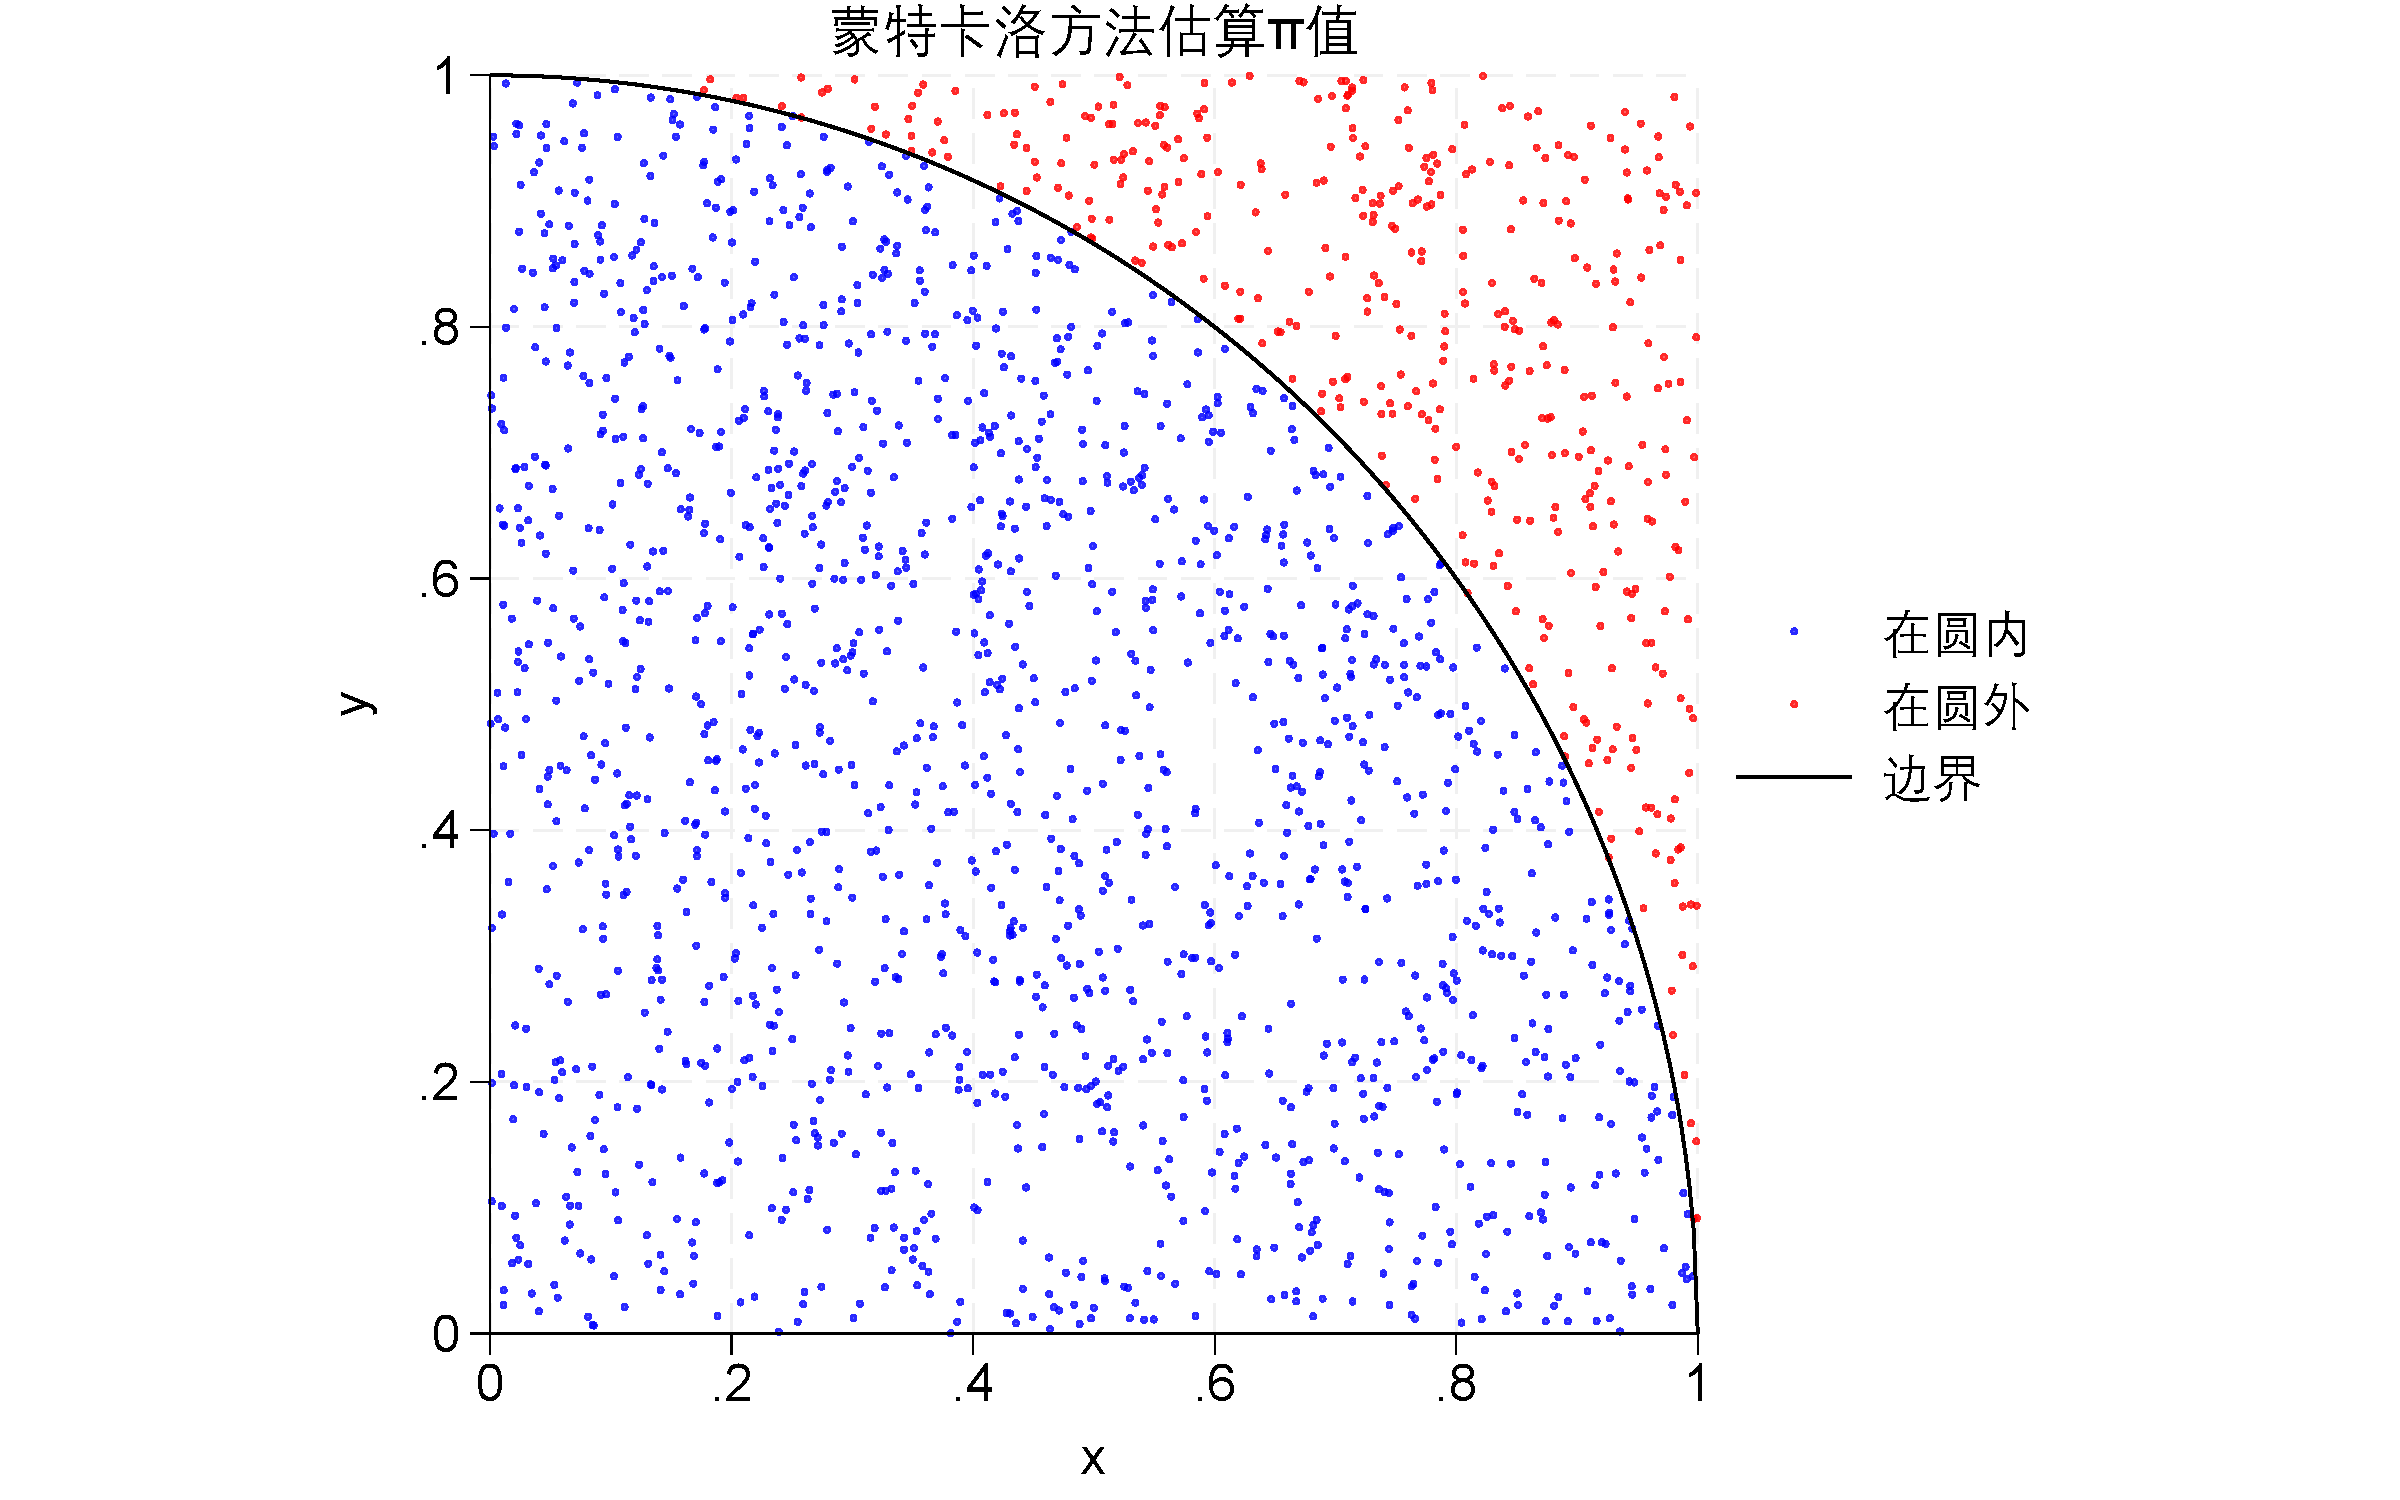
\includegraphics[width=0.8\textwidth]{image/circle_pi.pdf}
	\end{center}
\end{tcolorbox}

\begin{tcolorbox}[title=在 Stata 中运用模拟法验证大样本假定, colback=white, colframe=black, colbacktitle=white, coltitle=black,fonttitle=\bfseries]
	\begin{lstlisting}[xleftmargin=2em,
		basicstyle=\ttfamily\small\color{black},
		keywordstyle=\color{black},
		commentstyle=\color{black},
		stringstyle=\color{black},
		identifierstyle=\color{black},
		numberstyle=\color{black},
		showstringspaces=false,
		morekeywords={clear, set, seed, net, install, mc_ols_sim, from, replace, use, collapse, list, twoway, histogram, kdensity, line, title, legend, yline, xline, aspectratio, plotregion, graphregion, save, color}]
clear all // 清除内存中所有数据和程序
set seed 12345 // 设置随机数种子,确保结果可重现

// 安装ado文件
net install mc_ols_sim, from(https://gitee.com/yuanjingyang2/mc_ols_sim/raw/master) replace
// 运行蒙特卡洛模拟 - 不同样本容量
mc_ols_sim, n(10 30 50 100 200 500 700 1000) dist(poisson) reps(1000) beta0(1) beta1(0.2)
// 运行1000次模拟,样本量包含10-1000,其中的分布选项对应泊松

// 定义语法,n为样本量列表,dist为分布类型——默认为uniform,其中可选分布选项:uniform(均匀) normal(正态) binomial(二项) poisson(泊松) exponential(指数) cauchy(柯西) chi2(卡方),reps为模拟次数默认1000,beta0和beta1为回归系数默认值1和2。

// 分析结果 - 大数定律验证
use results.dta, clear // 调用存储的结果数据
collapse (mean) b0 b1, by(n) // 按样本量分组计算估计量均值
list // 显示结果

twoway (line b0 n, lcolor(blue) lpattern(solid)) ///  绘制截距估计均值线
       (line b1 n, lcolor(red) lpattern(solid)), ///  绘制斜率估计均值线
       yline(1 2, lpattern(dash) lcolor(black%20)) ///  添加真值参考线
       legend(order(1 "截距估计均值" 2 "斜率估计均值") pos(6) cols(3)) ///  添加图例
       title("大数定律:估计量收敛到真值") // 添加标题

// 分析结果 - 中心极限定理验证
use results.dta, clear // 重新调用数据

twoway ///
    (histogram b1 if n==10, width(0.1) percent color(blue%10) yaxis(1)) ///  n=10直方图
    (kdensity b1 if n==10, lcolor(blue) lwidth(medthick) yaxis(2)) ///  n=10核密度
    (histogram b1 if n==100, width(0.1) percent color(purple%10) yaxis(1)) ///  n=100直方图
    (kdensity b1 if n==100, lcolor(purple) lwidth(medthick) yaxis(2)) ///  n=100核密度
    (histogram b1 if n==1000, width(0.1) percent color(red%10) yaxis(1)) ///  n=1000直方图
    (kdensity b1 if n==1000, lcolor(red) lwidth(medthick) yaxis(2)), ///  n=1000核密度
    legend(order(4 "n=10" 5 "n=100" 6 "n=1000") pos(6) cols(3)) ///
    title("不同样本量下斜率估计量分布的对比") ///
    xtitle("斜率估计值") ///
    ytitle("百分比", axis(1)) ///
    ytitle("密度", axis(2))
	\end{lstlisting}
\end{tcolorbox}

\begin{tcolorbox}[title=在 Stata 中运用模拟法验证大样本假定, colback=white, colframe=black, colbacktitle=white, coltitle=black,fonttitle=\bfseries]

	\begin{center}
	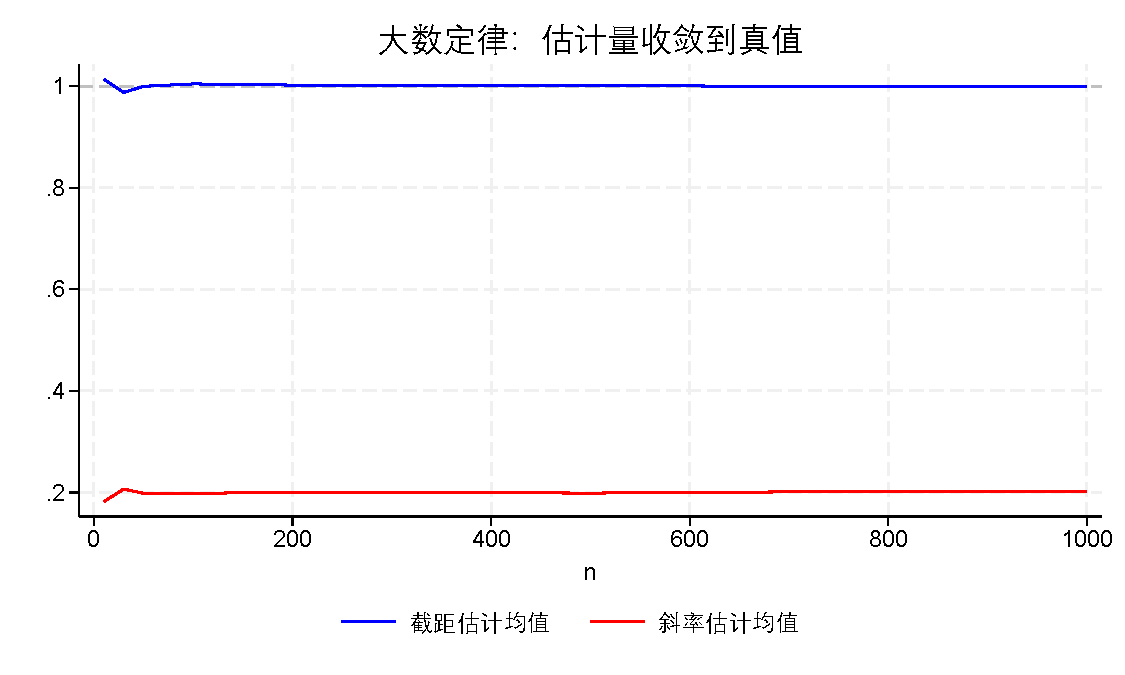
\includegraphics[width=0.8\textwidth]{image/large_numbers.pdf}
	\end{center}
	\begin{center}
	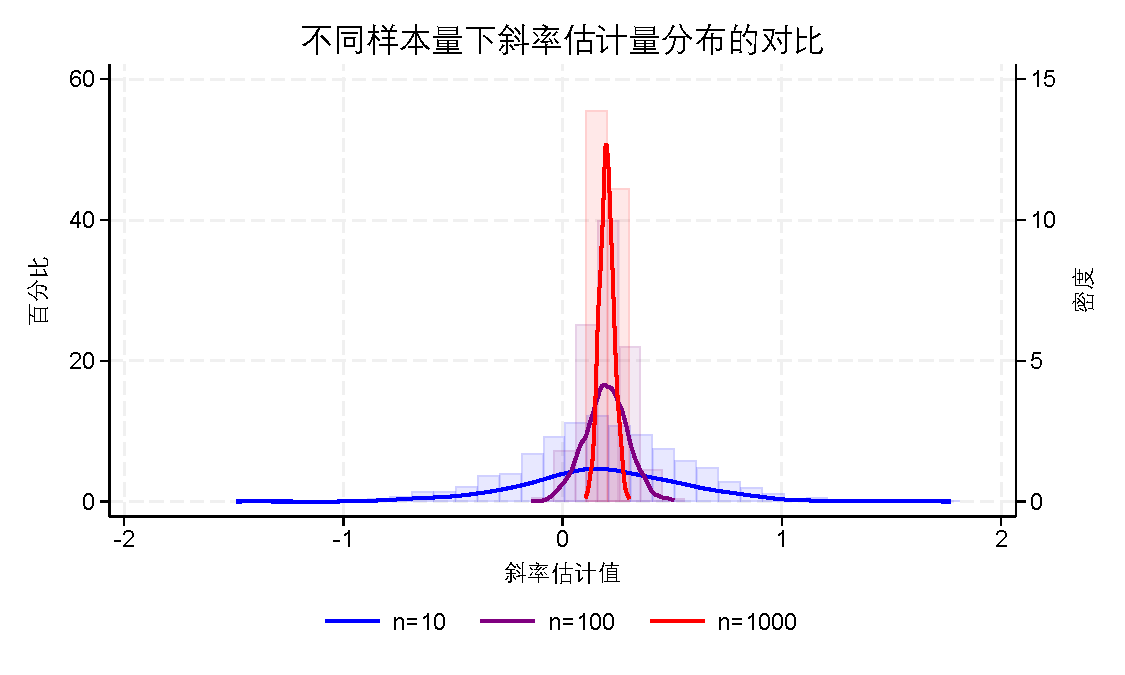
\includegraphics[width=0.8\textwidth]{image/central_limit.pdf}
	\end{center}
\end{tcolorbox}

\paragraph*{异方差问题}

在大多数计量经济学模型中,一个核心的假设是误差项的方差为常数,即满足同方差性(homoskedasticity)。然而,在许多现实世界的场景中,这一假设往往被违反,即误差项的方差会随着解释变量的变化而变化,此现象称为异方差性(heteroskedasticity)。异方差问题的存在导致普通最小二乘(OLS)估计量虽然仍是无偏且一致的,但不再是有效的(即不再具有最小方差),其计算的标准误会产生偏误,进而使基于这些标准误的假设检验(如t检验、F检验和Wald检验)以及置信区间失效,导致错误的统计推断。

我们通过一个模拟数据来展示异方差问题:

\begin{tcolorbox}[title=在 Stata 中展示异方差问题, colback=white, colframe=black, colbacktitle=white, coltitle=black,fonttitle=\bfseries]
	\begin{lstlisting}[xleftmargin=2em,
		basicstyle=\ttfamily\small\color{black},
		keywordstyle=\color{black},
		commentstyle=\color{black},
		stringstyle=\color{black},
		identifierstyle=\color{black},
		numberstyle=\color{black},
		showstringspaces=false,
		morekeywords={clear, set, seed, net, install, mc_ols_sim, from, replace, use, collapse, list, twoway, histogram, kdensity, line, title, legend, yline, xline, aspectratio, plotregion, graphregion, save, color}]
clear
set obs 500
set seed 12345

gen x = runiform(0, 10)
gen sigma = 0.5 + 0.5*x
gen u = rnormal(0, sigma)
gen y = 2 + 1.5*x + u

reg y x
predict resid, residuals
predict yhat, xb

twoway (scatter y x) (lfit y x), ///
    title("原始数据与拟合回归线") ///
    ytitle("y") ///
    xtitle("x") ///
    legend(order(1 "数据点" 2 "拟合线") cols(1) position(6)) ///
    name(graph1, replace)

twoway (scatter resid x) (lowess resid x, lcolor(red)), ///
    title("异方差诊断图") ///
    ytitle("残差") ///
    xtitle("x") ///
    legend(order(1 "残差点" 2 "局部加权回归线") cols(1) position(6)) ///
    name(graph2, replace)

graph combine graph1 graph2, cols(2) title("分析结果")
	\end{lstlisting}
	\vspace{2em}
	\begin{center}
	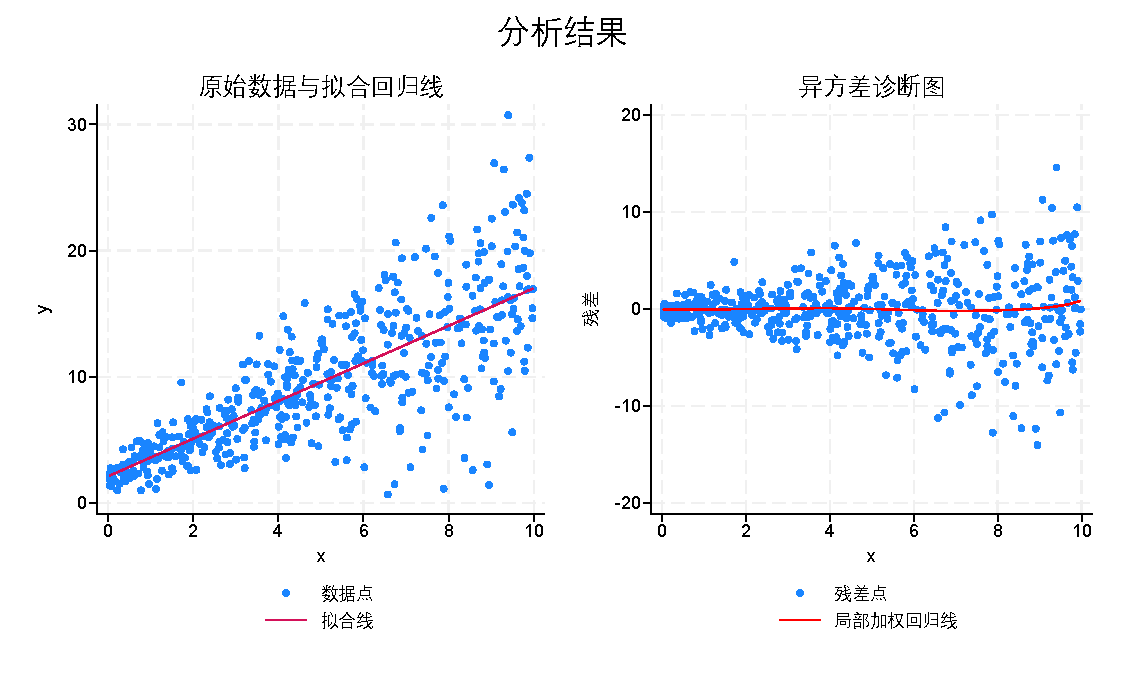
\includegraphics[width=0.8\textwidth]{image/heteroskedasticity.pdf}
	\end{center}
\end{tcolorbox}

\textbf{1. 异方差稳健标准误(Heteroskedasticity-Robust Standard Errors)}

在满足条件期望为零($\mathbb{E}[\epsilon_i|\bm{X}_i]=0$)但允许 $\mathrm{Var}(\epsilon_i|\bm{X}_i)=\sigma_i^2$ 随 $i$ 变化的情形下,OLS 点估计 $\hat{\bm{\beta}}=(\bm{X}'\bm{X})^{-1}\bm{X}'\bm{Y}$ 仍是一致的,但传统同方差方差公式 $s^2(\bm{X}'\bm{X})^{-1}$ 不再一致。White(1980)提出的异方差稳健(Eicker–Huber–White)协方差估计量在不预设异方差具体形式的前提下,给出对 $\mathrm{Var}(\hat{\bm{\beta}}|\bm{X})$ 的一致估计,从而保证大样本下的 $t$ 检验、Wald 检验与置信区间有效。

\textbf{数学推导}
在异方差下,OLS估计量的条件真方差为:

\begin{equation}
	\mathrm{Var}(\hat{\bm{\beta}}|\bm{X}) = (\bm{X}'\bm{X})^{-1}\bm{X}'\bm{\Omega}\bm{X}(\bm{X}'\bm{X})^{-1}
\end{equation}

其中,$\bm{\Omega} = \mathrm{diag}(\sigma_1^2,\dots,\sigma_n^2)$ 是误差项 $\bm{\epsilon}$ 的方差-协方差矩阵,它是一个对角矩阵,其对角线元素为各个观测点误差项的异方差。

White(1980)提出用 OLS 残差的平方 $\hat{e}_i^{\,2}$ 作为对未知异方差 $\sigma_i^2$ 的一致估计量。因此,对于中间的“夹心”部分 $\bm{X}'\bm{\Omega}\bm{X}$,我们可以用其样本类似物进行一致估计:

\begin{equation}
	\widehat{\bm{S}} = \sum_{i=1}^n \hat e_i^{\,2}\,\bm{X}_i\bm{X}_i'
\end{equation}

其中 $\bm{X}_i$ 是第 $i$ 个观测值的解释变量行向量(表示为列向量),$\hat e_i$ 是 OLS 残差。
将此样本类似物代入真方差公式,即可得到异方差稳健协方差的估计量:

\begin{equation}
	\begin{split}
		\widehat{\mathrm{Var}}_{\mathrm{robust}}(\hat{\bm{\beta}})
		&= (\bm{X}'\bm{X})^{-1}\left(\sum_{i=1}^n \hat e_i^{\,2}\,\bm{X}_i\bm{X}_i'\right)(\bm{X}'\bm{X})^{-1} \\
		&= (\bm{X}'\bm{X})^{-1}\bm{X}'\,\mathrm{diag}(\hat e_1^{\,2},\dots,\hat e_n^{\,2})\,\bm{X}\,(\bm{X}'\bm{X})^{-1}
	\end{split}
\end{equation}

这个结构常被形象地称作“三明治(sandwich)”形式:两侧的“面包”是 $(\bm{X}'\bm{X})^{-1}$,中间的“夹心”是 $\bm{X}'\,\mathrm{diag}(\hat e_1^{\,2},\dots,\hat e_n^{\,2})\,\bm{X}$。

\textbf{统计推断与报告}
令 $\widehat{\mathrm{Var}}_{\mathrm{robust}}(\hat{\bm{\beta}})=\hat{\bm{V}}$,则第 $k$ 个系数的稳健标准误为 $\mathrm{se}_k=\sqrt{\hat V_{kk}}$。
\begin{itemize}
  \item \textbf{不改变点估计}:异方差稳健标准误不改变原始OLS系数估计值,仅修正其标准误。
  \item \textbf{t 检验}:$t_k=\hat\beta_k/\mathrm{se}_k$。在大样本下,可用标准正态分布进行近似检验。
  \item \textbf{置信区间}:$\hat\beta_k \pm z_{1-\alpha/2}\,\mathrm{se}_k$(或在有限样本中用更保守的临界值)。
\end{itemize}
White 稳健标准误以简洁的三明治结构在不改变 OLS 点估计的前提下,为异方差环境下的大样本推断提供一致的标准误与检验基础,已成为应用计量经济学的“默认选项”之一。

在 Stata 中,可以通过 \texttt{robust} 选项实现:

\begin{tcolorbox}[title=在 Stata 中解决异方差问题, colback=white, colframe=black, colbacktitle=white, coltitle=black,fonttitle=\bfseries]
	\begin{lstlisting}[xleftmargin=2em,
		basicstyle=\ttfamily\small\color{black},
		keywordstyle=\color{black},
		commentstyle=\color{black},
		stringstyle=\color{black},
		identifierstyle=\color{black},
		numberstyle=\color{black},
		showstringspaces=false,
		morekeywords={clear, set, seed, net, install, mc_ols_sim, from, replace, use, collapse, list, twoway, histogram, kdensity, line, title, legend, yline, xline, aspectratio, plotregion, graphregion, save, color}]
clear
set obs 500
set seed 12345

gen x = runiform(0, 10)
gen sigma = 0.5 + 0.5*x
gen u = rnormal(0, sigma)
gen y = 2 + 1.5*x + u

reg y x
reg y x, robust
di "显然的,加入robust选项后x的标准误增加,t减小,即此时如果仍然显著,则更加稳健。"
	\end{lstlisting}
	\vspace{-1em}
	\begin{Verbatim}[commandchars=\\\{\},xleftmargin=2em]
. reg y x
      Source |       SS           df       MS      Number of obs   =       500
-------------+----------------------------------   F(1, 498)       =    772.97
       Model |  9384.67049         1  9384.67049   Prob > F        =    0.0000
    Residual |  6046.21789       498  12.1409998   R-squared       =    0.6082
-------------+----------------------------------   Adj R-squared   =    0.6074
       Total |  15430.8884       499   30.923624   Root MSE        =    3.4844

------------------------------------------------------------------------------
           y | Coefficient  Std. err.      t    P>|t|     [95% conf. interval]
-------------+----------------------------------------------------------------
           x |   1.490595   .0536139    27.80   0.000     1.385258    1.595933
       _cons |   2.120809   .3037144     6.98   0.000     1.524089    2.717528
------------------------------------------------------------------------------
. reg y x, robust
Linear regression                               Number of obs     =        500
                                                F(1, 498)         =     636.51
                                                Prob > F          =     0.0000
                                                R-squared         =     0.6082
                                                Root MSE          =     3.4844

------------------------------------------------------------------------------
             |               Robust
           y | Coefficient  std. err.      t    P>|t|     [95% conf. interval]
-------------+----------------------------------------------------------------
           x |   1.490595   .0590822    25.23   0.000     1.374514    1.606676
       _cons |   2.120809   .1961559    10.81   0.000     1.735414    2.506204
------------------------------------------------------------------------------
显然的,加入robust选项后x的标准误增加,t减小,即此时如果仍然显著,则更加稳健。
	\end{Verbatim}
\end{tcolorbox}

\textbf{2. 广义最小二乘法(Generalized Least Squares, GLS)}

广义最小二乘法(GLS)是处理异方差和(或)自相关问题的一种有效方法。其核心思想是:当误差项的方差—协方差矩阵不满足球形假设(即误差项既非同方差也非不相关)时,通过对模型进行线性变换,使得扰动项在转换后的模型中重新满足同方差和不相关性,进而利用OLS方法对转换后的模型进行估计。GLS不仅适用于异方差问题,也可推广至处理序列相关与更一般的相关结构。

\textbf{理论基础}

考虑线性回归模型:

\begin{equation}
	\bm{Y} = \bm{X}\bm{\beta} + \bm{\epsilon}
\end{equation}

其中 $\mathbb{E}(\bm{\epsilon}|\bm{X}) = \bm{0}$,但 $\mathrm{Var}(\bm{\epsilon}|\bm{X}) = \bm{\Omega}$,且 $\bm{\Omega} \neq \sigma^2 \bm{I}_n$。
GLS通过构造一个可逆的变换矩阵 $\bm{P}$,使得转换后的误差项 $\bm{\epsilon}^* = \bm{P}\bm{\epsilon}$ 满足球形扰动项假设,即 $\mathrm{Var}(\bm{\epsilon}^*|\bm{X}) = \sigma^2 \bm{I}_n$。

\textbf{数学推导}

我们寻找一个变换矩阵 $\bm{P}$,使得 $\mathrm{Var}(\bm{P}\bm{\epsilon}|\bm{X}) = \bm{P}\mathrm{Var}(\bm{\epsilon}|\bm{X})\bm{P}' = \bm{P}\bm{\Omega}\bm{P}' = \sigma^2 \bm{I}_n$。
若 $\bm{\Omega}$ 是一个正定矩阵,则其平方根逆矩阵 $\bm{P} = \bm{\Omega}^{-1/2}$ 存在。令 $\sigma^2=1$ 不失一般性(因为最终 $\sigma^2$ 会被估计并纳入方差),则选择 $\bm{P} = \bm{\Omega}^{-1/2}$,可以使:

\begin{equation}
	\begin{split}
		\mathrm{Var}(\bm{P}\bm{\epsilon}|\bm{X}) &= \bm{\Omega}^{-1/2} \bm{\Omega} (\bm{\Omega}^{-1/2})' \\
		&= \bm{\Omega}^{-1/2} \bm{\Omega} \bm{\Omega}^{-1/2} \\
		&= \bm{I}_n
	\end{split}
\end{equation}

对原始模型 $\bm{Y} = \bm{X}\bm{\beta} + \bm{\epsilon}$ 两边左乘 $\bm{P}$,得到转换后的模型:

\begin{equation}
	\bm{P}\bm{Y} = \bm{P}\bm{X}\bm{\beta} + \bm{P}\bm{\epsilon}
	\quad \text{或写为} \quad \bm{Y}^* = \bm{X}^*\bm{\beta} + \bm{\epsilon}^*
\end{equation}

其中 $\bm{Y}^*=\bm{P}\bm{Y}$,$\bm{X}^*=\bm{P}\bm{X}$,$\bm{\epsilon}^*=\bm{P}\bm{\epsilon}$。
此时,转换后的误差项 $\bm{\epsilon}^*$ 满足同方差和不相关性假设,因此可以对转换后的模型应用OLS,得到的估计量即为GLS估计量:

\begin{equation}
	\begin{split}
		\hat{\bm{\beta}}_{\mathrm{GLS}} &= ((\bm{P}\bm{X})'(\bm{P}\bm{X}))^{-1}(\bm{P}\bm{X})'(\bm{P}\bm{Y}) \\
		&= (\bm{X}'\bm{P}'\bm{P}\bm{X})^{-1}\bm{X}'\bm{P}'\bm{P}\bm{Y} \\
		&= (\bm{X}'\bm{\Omega}^{-1/2}\bm{\Omega}^{-1/2}\bm{X})^{-1}\bm{X}'\bm{\Omega}^{-1/2}\bm{\Omega}^{-1/2}\bm{Y} \\
		&= (\bm{X}'\bm{\Omega}^{-1}\bm{X})^{-1}\bm{X}'\bm{\Omega}^{-1}\bm{Y}
	\end{split}
\end{equation}

根据Gauss-Markov定理,$\hat{\bm{\beta}}_{\mathrm{GLS}}$ 是线性、无偏且有效的(BLUE)。

当 $\bm{\Omega}$ 未知时,需要通过某种方式对其进行估计,得到 $\hat{\bm{\Omega}}$。将 $\hat{\bm{\Omega}}$ 代替 $\bm{\Omega}$ 即可得到可行广义最小二乘(Feasible GLS, FGLS)估计量:

\begin{equation}
	\hat{\bm{\beta}}_{\mathrm{FGLS}} = (\bm{X}'\hat{\bm{\Omega}}^{-1}\bm{X})^{-1}\bm{X}'\hat{\bm{\Omega}}^{-1}\bm{Y}
\end{equation}

在正则条件下,FGLS具有与GLS相同的渐近性质,即渐近有效。

\textbf{与加权最小二乘(WLS)的关系}

当 $\bm{\Omega}$ 是一个对角矩阵(即仅存在异方差,无自相关)时,GLS估计量退化为加权最小二乘(Weighted Least Squares, WLS)估计量。此时,$\bm{\Omega}^{-1}$ 也是对角矩阵,其对角线元素为各观测值方差的倒数 $1/\sigma_i^2$,扮演了权重矩阵的角色。

\textbf{注意事项}
\begin{itemize}
\item GLS和FGLS要求对误差项的方差—协方差结构有正确的设定或准确的估计。若对 $\bm{\Omega}$ 的设定或估计有误,FGLS可能反而不如OLS(因社科数据通常难以完全掌握DGP,故很少使用)。
\item 在小样本情况下,由于 $\hat{\bm{\Omega}}$ 的估计误差,FGLS的表现不一定优于OLS。在大样本下,FGLS通常能显著提高估计的精度和效率。
\item 在实证研究中,若采用FGLS,应在转换并回归后重新检验异方差是否已被消除。
\end{itemize}

\textbf{3. 聚类稳健标准误(Cluster-Robust Standard Errors)}

在许多实证研究中,数据往往具有固有的群组(或集群)结构,例如来自同一学校的学生、同一公司内的员工,或同一地理区域的住户等。在这种情况下,同一群组内的观测值通常会受到共同的、未被模型捕获的因素影响,导致其误差项之间存在相关性。传统的普通最小二乘(OLS)标准误假设误差项是独立同分布的(i.i.d.),即使修正了异方差(如White标准误),也无法处理群组内部的相关性。忽略这种群组内的相关性会导致标准误被系统性低估,从而夸大估计结果的统计显著性,造成错误的推断。

聚类稳健标准误(Cluster-Robust Standard Errors, CRSE)旨在纠正这一问题。其核心思想是允许同一群组内的误差项存在任意形式的相关性(包括异方差和自相关),但假定不同群组间的误差项是相互独立的。在聚类稳健标准误下,OLS估计量 $\hat{\pmb{\beta}}^{\text{OLS}}$ 依然是无偏且一致的,但其标准误的计算方式需要调整。

\textbf{数学推导}

我们从OLS估计量方差的普遍形式出发:
\begin{equation}
	\operatorname{Var} \left( \hat{\pmb{\beta}}^{\text{OLS}} \right) = (\pmb{X}^{\prime}\pmb{X})^{-1} \pmb{X}^{\prime} E[\pmb{e}\pmb{e}^{\prime}] \pmb{X} (\pmb{X}^{\prime}\pmb{X})^{-1}
\end{equation}
其中,$\pmb{\Omega} = E[\pmb{e}\pmb{e}^{\prime}]$ 是误差项 $\pmb{e}$ 的方差-协方差矩阵。

在数据存在群组结构的情况下,假设总共有 $G$ 个群组,每个群组 $g$ 包含 $T_g$ 个观测值。我们将总的误差向量 $\pmb{e}$ 和解释变量矩阵 $\pmb{X}$ 相应地按群组进行划分:
\begin{equation}
	\pmb{e} = \begin{pmatrix} \pmb{e}_1 \\ \pmb{e}_2 \\ \vdots \\ \pmb{e}_G \end{pmatrix}, \quad \pmb{X} = \begin{pmatrix} \pmb{X}_1 \\ \pmb{X}_2 \\ \vdots \\ \pmb{X}_G \end{pmatrix}
\end{equation}
其中 $\pmb{e}_g$ 是第 $g$ 个群组的误差向量($T_g \times 1$),$\pmb{X}_g$ 是第 $g$ 个群组的解释变量矩阵($T_g \times K$,$K$ 为解释变量数量)。

聚类稳健标准误的核心假设是:群组间的误差项是相互独立的,而群组内的误差项可以任意相关。这意味着误差项的方差-协方差矩阵 $\pmb{\Omega}$ 呈现出块对角(block-diagonal)结构:
\begin{equation}
	\begin{split}
		\pmb{\Omega}_{\text{cluster}} = E[\pmb{e}\pmb{e}^{\prime}] \\
		&= \begin{pmatrix} 
		E[\pmb{e}_1\pmb{e}_1^{\prime}] & \pmb{0} & \cdots & \pmb{0} \\
		\pmb{0} & E[\pmb{e}_2\pmb{e}_2^{\prime}] & \cdots & \pmb{0} \\
		\vdots & \vdots & \ddots & \vdots \\
		\pmb{0} & \pmb{0} & \cdots & E[\pmb{e}_G\pmb{e}_G^{\prime}]
		\end{pmatrix} \\
		&= \operatorname{diag}(\pmb{\Omega}_1, \pmb{\Omega}_2, \dots, \pmb{\Omega}_G)
	\end{split}
\end{equation}
其中 $\pmb{\Omega}_g = E[\pmb{e}_g\pmb{e}_g^{\prime}]$ 是第 $g$ 个群组的误差项方差-协方差矩阵,它允许非对角线元素非零,即群组内部存在相关性。

将此块对角矩阵代入OLS估计量的方差公式:
\begin{equation}
	\begin{split}
		\operatorname{Var} \left( \hat{\pmb{\beta}}^{\text{OLS}} \right) &= (\pmb{X}^{\prime}\pmb{X})^{-1} \pmb{X}^{\prime} \pmb{\Omega}_{\text{cluster}} \pmb{X} (\pmb{X}^{\prime}\pmb{X})^{-1} \\
		&= (\pmb{X}^{\prime}\pmb{X})^{-1} \left( \sum_{g=1}^{G} \pmb{X}_g^{\prime} \pmb{\Omega}_g \pmb{X}_g \right) (\pmb{X}^{\prime}\pmb{X})^{-1}
	\end{split}
\end{equation}
为了估计这个方差,我们用样本残差 $\hat{\pmb{e}}_g = \pmb{Y}_g - \pmb{X}_g \hat{\pmb{\beta}}^{\text{OLS}}$ 来近似 $\pmb{e}_g$,并用样本协方差 $\hat{\pmb{e}}_g \hat{\pmb{e}}_g^{\prime}$ 来近似真实的 $\pmb{\Omega}_g = E[\pmb{e}_g\pmb{e}_g^{\prime}]$。因此,聚类稳健标准误的估计公式为:
\begin{equation}
	\widehat{\operatorname{Var}} \left( \hat{\pmb{\beta}}_{\text{cluster}}^{\text{OLS}} \right) = (\pmb{X}^{\prime}\pmb{X})^{-1} \left[ \sum_{g=1}^{G} \pmb{X}_{g}^{\prime} \hat{\pmb{e}}_{g} \hat{\pmb{e}}_{g}^{\prime} \pmb{X}_{g} \right] (\pmb{X}^{\prime}\pmb{X})^{-1}
\end{equation}
在实际应用中,通常还会加入小样本调整项,例如乘以 $\frac{G}{G-1}$ 或 $\frac{N-1}{N-K} \frac{G}{G-1}$,其中 $N$ 是总观测数,$K$ 是解释变量的数量。

\textbf{使用须知}

聚类稳健标准误允许误差项在群组内任意相关和异方差,但在群组间保持独立。它在群组数量 $G$ 足够大时(通常认为至少20-30个群组)是OLS估计量方差的一致估计。当群组数量过少时,聚类稳健标准误可能表现不佳。因此,在选择聚类标准误时,研究者需要仔细考虑群组的定义以及群组的数量。

在 Stata 中,可以使用 \texttt{cluster} 选项实现,例如按组变量 \texttt{groupid} 聚类:

\begin{tcolorbox}[title=在 Stata 中实现加权-聚类稳健标准误, colback=white, colframe=black, colbacktitle=white, coltitle=black,fonttitle=\bfseries]
	\begin{lstlisting}[xleftmargin=2em,
		basicstyle=\ttfamily\small\color{black},
		keywordstyle=\color{black},
		commentstyle=\color{black},
		stringstyle=\color{black},
		identifierstyle=\color{black},
		numberstyle=\color{black},
		showstringspaces=false,
		morekeywords={clear, set, seed, net, install, mc_ols_sim, from, replace, use, collapse, list, twoway, histogram, kdensity, line, title, legend, yline, xline, aspectratio, plotregion, graphregion, save, color, table}]
// 生成同时具有异方差和聚类相关性的数据
clear all
qui set obs 1500

// 生成聚类结构
gen group_id = ceil(_n/5)  // 300个组,每组5个观测
gen x1 = rnormal(0,1)
gen x2 = rnormal(0,1)
gen z = runiform(0,1)

// 生成异方差结构
gen sigma = exp(0.3*z)  // 异方差结构
gen group_fe = rnormal(0,0.3)  // 组层面固定效应

// 扩展组固定效应到所有观测
qui bysort group_id: replace group_fe = group_fe[1]

// 生成误差项
gen e = rnormal(0,sigma)
gen y = 1 + 2*x1 + 1.5*x2 + group_fe + e  // 真实模型

// 第一步:普通OLS
qui reg y x1 x2
estimates store ols

// 第二步:估计异方差结构
qui predict resid, residuals  // 获取残差
gen log_resid2 = log(resid^2)  // 残差平方的对数
qui reg log_resid2 z  // 回归估计方差函数
qui predict fitted_log_resid2  // 预测log(σ²)
gen estimated_sigma = sqrt(exp(fitted_log_resid2))  // 估计σ
gen weights = 1/(estimated_sigma^2)  // 计算权重

// 第三步:加权最小二乘
qui reg y x1 x2 [aweight=weights]
estimates store wls

// 第四步:聚类稳健标准误
qui reg y x1 x2, cluster(group_id)
estimates store clustered_se

// 第五步:同时使用权重和聚类稳健标准误
qui reg y x1 x2 [aweight=weights], cluster(group_id)
estimates store wls_clustered

// 比较所有结果
estimates table ols wls clustered_se wls_clustered, b(%9.4f) se stats(N r2)
\end{lstlisting}
\end{tcolorbox}

\begin{tcolorbox}[title=在 Stata 中实现加权-聚类稳健标准误, colback=white, colframe=black, colbacktitle=white, coltitle=black,fonttitle=\bfseries]

	\begin{Verbatim}[commandchars=\\\{\},xleftmargin=2em]
. estimates table ols wls clustered_se wls_clustered, b(%9.4f) se stats(N r2)
--------------------------------------------------------------
    Variable |    ols         wls      cluster~e   wls_clu~d  
-------------+------------------------------------------------
          x1 |    1.9715      1.9738      1.9715      1.9738  
             |    0.0322      0.0320      0.0313      0.0310  
          x2 |    1.4718      1.4713      1.4718      1.4713  
             |    0.0320      0.0318      0.0317      0.0314  
       _cons |    0.9053      0.9058      0.9053      0.9058  
             |    0.0317      0.0316      0.0356      0.0354  
-------------+------------------------------------------------
           N |      1500        1500        1500        1500  
          r2 |    0.7985      0.8005      0.7985      0.8005  
--------------------------------------------------------------
                                                  Legend: b/se

	\end{Verbatim}

\end{tcolorbox}

\section{非OLS回归与时空计量经济学}

当古典线性回归模型的假定(特别是关于误差项的假定)不再成立时,我们需要转向更广义的回归方法。本节将介绍当因变量为离散或受限类型,以及当数据包含时间或空间维度时所采用的专门模型。这些模型扩展了统计推断的边界,使其能够处理更复杂的社会科学问题。

\subsection{离散与受限因变量}

在许多研究中,因变量并非连续变量,而是表现为类别、计数或在某个范围内受限的形式。例如,投票选择(支持/反对)、事故发生次数或家庭耐用品支出(不能为负)。在这种情况下,使用普通最小二乘法(OLS)是不恰当的,因为它可能产生无意义的预测(如概率大于1或小于0),并且其线性假定本身也存在问题。

\paragraph*{线性概率模型(LPM)的局限}
对于二元因变量(取值为0或1),最简单的方法是使用OLS,这被称为\textbf{线性概率模型(Linear Probability Model, LPM)}。尽管LPM的系数易于解释(表示自变量变化一单位,因变量取1的概率变化多少),但它存在严重缺陷:
\begin{enumerate}
    \item \textbf{预测概率越界}:LPM的拟合值(即预测概率)可能超出[0, 1]的合理范围。
    \item \textbf{非线性关系}:自变量对概率的边际效应通常不是恒定的,而LPM假设其为线性。
    \item \textbf{异方差性}:当因变量为0-1分布时,误差项的方差依赖于解释变量的值,即
    \[
    \text{Var}(\varepsilon_i | \mathbf{X}) = p_i(1-p_i)
    \]
    这违反了同方差假定。
\end{enumerate}

为了克服这些问题,我们需要使用专门为离散或受限因变量设计的非线性模型。

\paragraph*{二元选择模型:Logit与Probit}
当因变量是二元选择时(如是否就业、是否投票),通常使用\textbf{Logit模型}和\textbf{Probit模型}。这两种模型都通过一个非线性的累积分布函数(Cumulative Distribution Function, CDF)将自变量的线性组合映射到(0, 1)区间,从而保证预测概率的有效性。

\textbf{Logit模型}假设潜在误差项服从Logistic分布(Logistic Distribution)。其概率表达式为:
\begin{equation}
P(Y_i=1 | \mathbf{X}_i) = \Lambda(\mathbf{X}_i'\boldsymbol{\beta}) = \frac{\exp(\mathbf{X}_i'\boldsymbol{\beta})}{1 + \exp(\mathbf{X}_i'\boldsymbol{\beta})}
\end{equation}
其中 $\Lambda(\cdot)$ 是Logistic分布的CDF。Logit模型的系数可以解释为对数几率(log-odds ratio)的变化。

\textbf{Probit模型}假设潜在误差项服从标准正态分布。其概率表达式为:
\begin{equation}
P(Y_i=1 | \mathbf{X}_i) = \Phi(\mathbf{X}_i'\boldsymbol{\beta}) = \int_{-\infty}^{\mathbf{X}_i'\boldsymbol{\beta}} \frac{1}{\sqrt{2\pi}} \exp\left(-\frac{z^2}{2}\right) dz
\end{equation}
其中 $\Phi(\cdot)$ 是标准正态CDF。

由于模型的非线性,Logit和Probit模型的系数本身并不直接等于边际效应。我们需要计算\textbf{平均边际效应(Average Marginal Effects, AME)}来解释自变量对概率的影响。

\begin{figure}[htbp]
	\centering
	\fbox{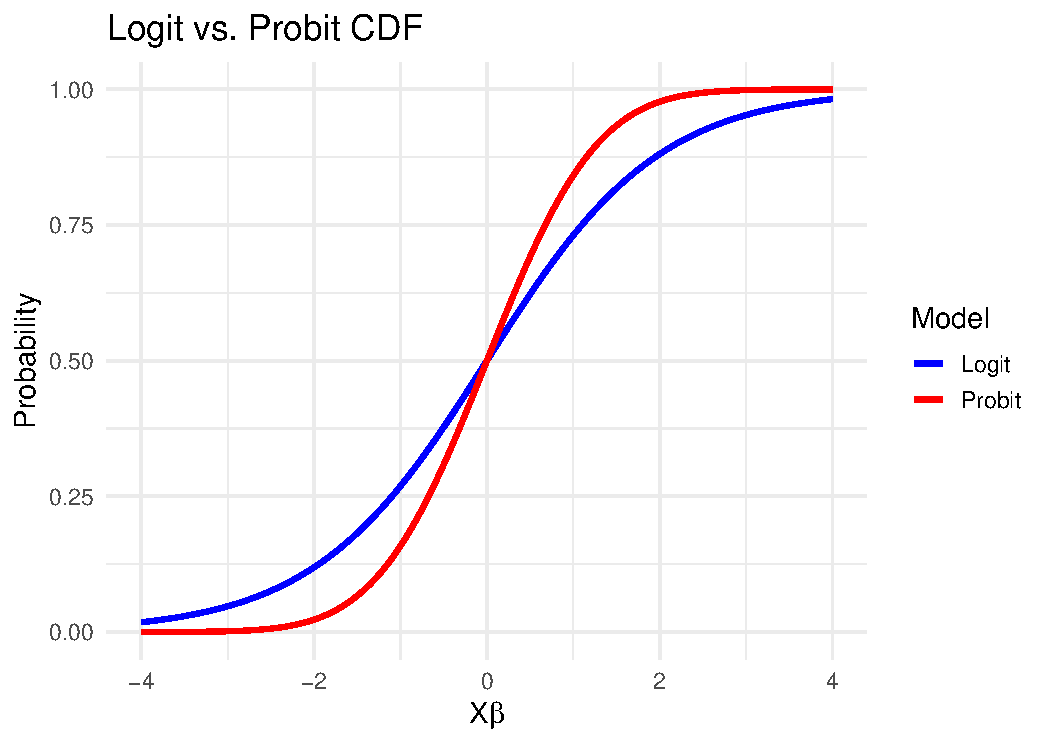
\includegraphics[width=0.7\textwidth]{image/logit_probit_cdf.pdf}}
	\caption[两个分布的CDF]{两个分布的CDF}
	\label{fig:logit_probit_cdf}
\end{figure}

\begin{tcolorbox}[title=在 Stata 中估计 Probit 模型并计算边际效应, colback=white, colframe=black, colbacktitle=white, coltitle=black,fonttitle=\bfseries]
\begin{lstlisting}[xleftmargin=2em, commentstyle=\color{black}]
quietly sysuse auto, clear

*线性模型
qui regress foreign mpg weight
est store lpm

*Logit 模型
qui logit foreign mpg weight
est store logit_model
margins, dydx(*) // 计算平均边际效应

*Probit 模型
qui probit foreign mpg weight
est store probit_model
margins, dydx(*) // 计算平均边际效应
est table lpm logit_model probit_model, b(%9.4f) se stats(N ll)
\end{lstlisting}
\vspace{-2em}
\begin{Verbatim}[commandchars=\\\{\},xleftmargin=2em]

*Probit模型的边际效应与输出表格

------------------------------------------------------------------------------
             |            Delta-method
             |      dy/dx   std. err.      z    P>|z|     [95% conf. interval]
-------------+----------------------------------------------------------------
         mpg |  -.0206923      .0092    -2.25   0.025    -.0387239   -.0026607
      weight |  -.0004649   .0000565    -8.23   0.000    -.0005756   -.0003542
------------------------------------------------------------------------------

------------------------------------------------------------
                      (1)             (2)             (3)   
                  foreign         foreign         foreign   
------------------------------------------------------------
main                                                        
mpg               -0.0194         -0.1686         -0.1040*  
                 (0.0127)        (0.0919)        (0.0516)   

weight            -0.0005***      -0.0039***      -0.0023***
                 (0.0001)        (0.0010)        (0.0006)   

_cons              2.1235***      13.7084**        8.2755** 
                 (0.5290)        (4.5187)        (2.5541)   
------------------------------------------------------------
N                 74.0000         74.0000         74.0000   
ll               -29.8382        -27.1752        -26.8442   
------------------------------------------------------------
Standard errors in parentheses
* p<0.05, ** p<0.01, *** p<0.001

\end{Verbatim}
\end{tcolorbox}

从Logit模型的边际效应结果看,车重(weight)每增加1个单位,汽车为进口车的概率平均下降约0.0004569。

\paragraph*{计数数据模型:泊松回归}
当因变量是表示事件发生次数的非负整数时(如专利申请数、罢工次数),\textbf{泊松回归(Poisson Regression)}是常用的模型。它假设在给定自变量的条件下,因变量服从泊松分布。其核心是条件期望函数:
\begin{equation}
E(Y_i | \mathbf{X}_i) = \lambda_i = \exp(\mathbf{X}_i'\boldsymbol{\beta})
\end{equation}
使用指数函数形式可以确保预测的期望值为正。泊松分布的一个关键假设是均值与方差相等,即
\[
E(Y_i)=Var(Y_i)
\]
如果数据表现出\textbf{过度分散(Overdispersion)},即方差远大于均值,则应使用\textbf{负二项回归(Negative Binomial Regression)}模型,它引入了一个额外的参数来解释过度分散。

\paragraph*{受限因变量模型:Tobit回归}
当因变量在一个点上(通常是0)被\textbf{删失(Censored)}时,即我们只能观察到变量大于等于0的值,而小于0的值都被记录为0时,应使用\textbf{Tobit模型}。例如,家庭的汽车支出,对于不买车的家庭,该值为0。Tobit模型假设存在一个潜在的连续变量 $Y_i^*$,它由线性模型决定:
\begin{equation}
Y_i^* = \mathbf{X}_i'\boldsymbol{\beta} + \varepsilon_i, \quad \varepsilon_i \sim N(0, \sigma^2)
\end{equation}
而我们观测到的 $Y_i$ 是:
\begin{equation}
Y_i =
\begin{cases}
Y_i^* & \text{if } Y_i^* > 0 \\
0 & \text{if } Y_i^* \leq 0
\end{cases}
\end{equation}

使用OLS估计此类数据会导致系数估计有偏,而Tobit模型通过最大似然估计法可以得到一致的估计量。

为节省篇幅,我们这里只给出了Stata官方文档中的一些操作方法,更多内容请参考Stata官方文档。

\begin{itemize}
	\item \href{https://www.stata.com/manuals13/rpoisson.pdf}{泊松回归}
	\item \href{https://www.stata.com/manuals13/rnbreg.pdf}{负二项回归}
	\item \href{https://www.stata.com/manuals14/rtobit.pdf}{Tobit回归}
\end{itemize}

\begin{tcolorbox}[title=在 Stata 中估计 Poisson 模型和负二项模型, colback=white, colframe=black, colbacktitle=white, coltitle=black,fonttitle=\bfseries]
\begin{lstlisting}[xleftmargin=2em, commentstyle=\color{black}]
quietly webuse dollhill3, clear
* 使用 poisson 回归来处理过度分散
poisson deaths smokes i.agecat, exposure(pyears) irr
estat gof // 假设结果显著提示过度分散
* 使用负二项回归来处理过度分散(不太对)
nbreg deaths smokes i.agecat, exposure(pyears) irr
\end{lstlisting}
\vspace{-2em}
\begin{Verbatim}[commandchars=\\\{\},xleftmargin=2em]

------------------------------------------------------------------------------
      deaths |        IRR   Std. err.      z    P>|z|     [95% conf. interval]
-------------+----------------------------------------------------------------
      smokes |   1.425519   .1530638     3.30   0.001     1.154984    1.759421
             |
      agecat |
      45–54  |   4.410584   .8605197     7.61   0.000     3.009011    6.464997
      55–64  |    13.8392   2.542638    14.30   0.000     9.654328    19.83809
      65–74  |   28.51678   5.269878    18.13   0.000     19.85177    40.96395
      75–84  |   40.45121   7.775511    19.25   0.000     27.75326    58.95885
             |
       _cons |   .0003636   .0000697   -41.30   0.000     .0002497    .0005296
  ln(pyears) |          1  (exposure)
------------------------------------------------------------------------------
Note: _cons estimates baseline incidence rate.

         Deviance goodness-of-fit =  12.13237
         Prob > chi2(4)           =    0.0164

         Pearson goodness-of-fit  =  11.15533
         Prob > chi2(4)           =    0.0249

------------------------------------------------------------------------------
      deaths |        IRR   Std. err.      z    P>|z|     [95% conf. interval]
-------------+----------------------------------------------------------------
      smokes |   1.425519   .1530638     3.30   0.001     1.154984    1.759422
             |
      agecat |
      45–54  |   4.410584   .8605198     7.61   0.000     3.009011    6.464998
      55–64  |    13.8392   2.542639    14.30   0.000     9.654327    19.83809
      65–74  |   28.51678   5.269879    18.13   0.000     19.85177    40.96396
      75–84  |    40.4512   7.775512    19.25   0.000     27.75325    58.95885
             |
       _cons |   .0003636   .0000697   -41.30   0.000     .0002497    .0005296
  ln(pyears) |          1  (exposure)
-------------+----------------------------------------------------------------
    /lnalpha |  -18.68104   732.0311                     -1453.436    1416.074
-------------+----------------------------------------------------------------
       alpha |   7.71e-09   5.64e-06                             0           .
------------------------------------------------------------------------------

\end{Verbatim}
\end{tcolorbox}

\begin{tcolorbox}[title=在 Stata 中估计 Tobit 模型, colback=white, colframe=black, colbacktitle=white, coltitle=black,fonttitle=\bfseries]
\begin{lstlisting}[xleftmargin=2em, commentstyle=\color{black}]
quietly webuse mroz87, clear
tab whrs75 if whr < 50
tobit whrs75 nwinc wedyrs wexper c.wexper#c.wexper wifeage kl6 k618, ll(0)
\end{lstlisting}
\vspace{-2em}
\begin{Verbatim}[commandchars=\\\{\},xleftmargin=2em]

     Wife's |
   hours of |
    work in |
       1975 |      Freq.     Percent        Cum.
------------+-----------------------------------
          0 |        325       98.19       98.19
         12 |          1        0.30       98.49
         15 |          2        0.60       99.09
         30 |          1        0.30       99.40
         44 |          1        0.30       99.70
         48 |          1        0.30      100.00
------------+-----------------------------------
      Total |        331      100.00


-----------------------------------------------------------------------------------
           whrs75 | Coefficient  Std. err.      t    P>|t|     [95% conf. interval]
------------------+----------------------------------------------------------------
            nwinc |  -8.814227   4.459089    -1.98   0.048    -17.56808   -.0603708
           wedyrs |   80.64541   21.58318     3.74   0.000     38.27441    123.0164
           wexper |    131.564   17.27935     7.61   0.000     97.64211     165.486
                  |
c.wexper#c.wexper |  -1.864153   .5376606    -3.47   0.001    -2.919661   -.8086455
                  |
          wifeage |  -54.40491   7.418483    -7.33   0.000     -68.9685   -39.84133
              kl6 |  -894.0202   111.8777    -7.99   0.000    -1113.653   -674.3875
             k618 |  -16.21805    38.6413    -0.42   0.675    -92.07668    59.64057
            _cons |   965.3068   446.4351     2.16   0.031     88.88827    1841.725
------------------+----------------------------------------------------------------
     var(e.whrs75)|    1258927   93304.48                       1088458     1456093
-----------------------------------------------------------------------------------

\end{Verbatim}
\end{tcolorbox}

这样,我们基本完成了误差项和因变量与标准OLS回归状态下分布不同的回归估计介绍,下面我们进入一个有趣、也是在金融学领域中很深入的话题——时间序列分析。

\subsection{时间序列分析}

时间序列数据是按时间顺序排列的一系列观测值。与截面数据不同,时间序列数据的观测值之间通常存在依赖关系,即当前值会受到过去值的影响。这种\textbf{序列相关性(Serial Correlation)}或\textbf{自相关性(Autocorrelation)}是时间序列分析的核心。

在政治学和社会学的历史制度主义领域之中,时间序列的这种历时相关性有一个更为深刻且常见的理论表达——\textbf{路径依赖}。这一概念强调,历史的偶然事件或早期选择会通过自我强化机制(如规模报酬递增、协调效应等),将后续的制度变迁或政策发展锁定在某一个特定的轨道上,即使存在更优的替代方案。

从统计学的角度看,路径依赖正是时间序列数据中序列相关性的深刻体现。一个具有强自相关的过程,意味着其当前状态在很大程度上由其过去状态所决定,这与“历史塑造未来”的理念不谋而合。特别地,当一个时间序列存在\textbf{单位根}时,它表现出一种极端的路径依赖:历史上的任何一次冲击(shock)所造成的影响都是永久性的,不会随着时间的推移而消散。这为理解政治制度(如选举制度的演变)或长期政策(如福利国家的形成)的“锁定效应”(与“关键节点”提供了有力的量化分析工具。因此,检验时间序列的平稳性,实际上也是在探究我们所研究的政治或社会过程在多大程度上受到其自身历史的束缚。

为了理解时间序列,我们通常从基础的单变量时间序列模型开始。

\textbf{自回归模型 (AR)}

上述用于检验单位根的一阶自回归模型 AR(1) 是更广泛的\textbf{自回归模型 (Autoregressive Model, AR)} 的一个特例。一个 $p$ 阶的自回归模型 AR($p$) 表示,序列的当前值是其过去 $p$ 个值的线性组合加上一个随机扰动项。其一般形式为:
\begin{equation}
	Y_t = c + \phi_1 Y_{t-1} + \phi_2 Y_{t-2} + \dots + \phi_p Y_{t-p} + \varepsilon_t
\end{equation}
其中 $c$ 是常数项,$\phi_1, \dots, \phi_p$ 是自回归系数,$\varepsilon_t$ 是白噪声。AR模型捕捉了序列自身的“记忆”或持续性。在AR(1)模型 $Y_t = \rho Y_{t-1} + \varepsilon_t$ 中,如果 $|\rho|<1$,序列是平稳的;如果 $\rho=1$,序列就含有单位根,是一个随机游走过程,其方差随时间无限增大。我们可以通过\textbf{增广迪基-福勒检验(Augmented Dickey-Fuller, ADF)}来检验序列中是否存在单位根。

\textbf{移动平均模型 (MA)}

与AR模型不同,\textbf{移动平均模型 (Moving Average Model, MA)} 认为序列的当前值受到当前和过去的随机扰动项(或称“冲击”)的影响。一个 $q$ 阶的移动平均模型 MA($q$) 的形式为:
\begin{equation}
	Y_t = \mu + \varepsilon_t + \theta_1 \varepsilon_{t-1} + \theta_2 \varepsilon_{t-2} + \dots + \theta_q \varepsilon_{t-q}
\end{equation}
其中 $\mu$ 是序列的均值,$\theta_1, \dots, \theta_q$ 是移动平均系数。MA模型擅长刻画那些在受到一次冲击后,影响会持续几期然后完全消失的事件。例如,一次性的政策公告可能在短期内影响公众情绪,但其效果不会无限持续。

\textbf{ARMA 与 ARIMA 模型}

在实际应用中,许多时间序列同时表现出AR和MA过程的特征。因此,可以将两者结合起来,形成\textbf{自回归移动平均模型 (Autoregressive Moving Average Model, ARMA($p,q$))}:
\begin{equation}
	Y_t = c + \phi_1 Y_{t-1} + \dots + \phi_p Y_{t-p} + \varepsilon_t + \theta_1 \varepsilon_{t-1} + \dots + \theta_q \varepsilon_{t-q}
\end{equation}
然而,AR、MA和ARMA模型都要求时间序列是平稳的。对于含有单位根的非平稳序列,经典的\textbf{Box-Jenkins方法}要求先对其进行\textbf{差分(Differencing)}以实现平稳。如果一个序列经过 $d$ 次差分后变为平稳的ARMA($p,q$)过程,则称原序列服从\textbf{自回归差分移动平均模型 (Autoregressive Integrated Moving Average Model, ARIMA($p,d,q$))}。这里的 $d$ 就是“整合”的阶数(Integrated order),代表了序列中单位根的个数。

\textbf{选择AR、MA还是ARMA模型}

我们通过画自相关和偏自相关系数图来确定是AR还是MA模型,如果ac拖尾,pac截尾,那么是AR模型,再看这个图是几期后截尾的,如第一期时为0.8,第二阶突然掉到0附近,且再没恢复,那么就是一阶的;反之则为MA模型,阶数判断方法同理。图\ref{fig:acf_pac}展示了一个AR(1)模型的自相关和偏自相关系数图。

ARMA(p,q)也是一个道理,只不过具体的定阶用的是信息准则,画图时候可以发现两个都是拖尾时候就适合用ARMA模型了。

\textbf{平稳性与单位根}

时间序列分析的一个基本概念是\textbf{平稳性(Stationarity)}。一个弱平稳的时间序列,其均值、方差和任意滞后阶的自协方差不随时间变化。非平稳序列(如带有趋势的GDP)直接用于回归分析,可能导致\textbf{伪回归(Spurious Regression)},即两个不相关的序列可能表现出很高的 $R^2$ 和显著的t统计量。

一个常见的非平稳来源是\textbf{单位根(Unit Root)},对一个简单的一阶自回归模型 AR(1) 来说:

\begin{equation}
	Y_t = \rho Y_{t-1} + \varepsilon_t
\end{equation}

如果 $|\rho|<1$,序列是平稳的;如果 $\rho=1$,序列就含有单位根,是一个随机游走过程,其方差随时间无限增大。我们可以通过\textbf{增广迪基-福勒检验(Augmented Dickey-Fuller, ADF)}来检验序列中是否存在单位根。

\href{https://doi.org/10.1080/07350015.1989.10509723}{Schwert(1989)}
建议最大滞后阶数为:  
\begin{equation}
  \mu = \left\lfloor 12 \cdot \left( \frac{T}{100} \right)^{1/4} \right\rfloor  
\end{equation}

在此基础上,我们继续使用信息准则法进行判断,所谓信息准则,可以粗略理解为模型准确性与复杂度之间关系的度量,越复杂的模型准确性越高,但单个变量参数值的方差可能较大,因此引入信息准则来平衡滞后期数与准确性之间的矛盾。

\textbf{协整与误差修正模型}

如果两个或多个非平稳序列(通常是I(1)序列,即一阶差分后平稳)的某个线性组合是平稳的,那么这些序列之间存在\textbf{协整(Cointegration)}关系。这表明它们之间存在一个稳定的长期均衡关系。例如,收入和消费都是非平稳的,但它们之间存在长期均衡。

当协整关系存在时,我们可以使用\textbf{误差修正模型(Error Correction Model, ECM)}来同时捕捉变量间的长期均衡和短期动态调整。ECM的形式为:

\begin{equation}
\Delta Y_t = \alpha_0 + \alpha_1 (Y_{t-1} - \beta_1 - \beta_2 X_{t-1}) + \gamma_1 \Delta X_t + \varepsilon_t
\end{equation}

其中,$(Y_{t-1} - \beta_1 - \beta_2 X_{t-1})$ 是上一期的\textbf{误差修正项},代表对长期均衡的偏离。系数 $\alpha_1$(应为负值)表示每期调整回均衡状态的速度。

\textbf{向量自回归模型 (VAR)}

当分析多个时间序列变量之间的相互动态关系时,单方程模型就显得力不从心。向量自回归(Vector Autoregression, VAR)模型是单变量自回归(AR)模型向多元变量系统的推广。在VAR模型中,系统内的每一个内生变量都作为其自身以及所有其他内生变量的滞后值的函数来建模,从而捕捉了变量间复杂的动态联系。

对于一个一般的 $k$ 变量 VAR($p$) 模型,其展开的方程组形式如下。系统中的第1个、第2个直到第 $k$ 个方程分别为:

\begin{equation}
\begin{aligned}
y_{1,t} = c_1 &+ \left( \phi_{11}^{(1)} y_{1,t-1} + \phi_{12}^{(1)} y_{2,t-1} + \dots + \phi_{1k}^{(1)} y_{k,t-1} \right) \\
              &+ \left( \phi_{11}^{(2)} y_{1,t-2} + \phi_{12}^{(2)} y_{2,t-2} + \dots + \phi_{1k}^{(2)} y_{k,t-2} \right) \\
              &+ \dots \\
              &+ \left( \phi_{11}^{(p)} y_{1,t-p} + \phi_{12}^{(p)} y_{2,t-p} + \dots + \phi_{1k}^{(p)} y_{k,t-p} \right) \\
              &+ \varepsilon_{1,t} \\
y_{2,t} = c_2 &+ \left( \phi_{21}^{(1)} y_{1,t-1} + \phi_{22}^{(1)} y_{2,t-1} + \dots + \phi_{2k}^{(1)} y_{k,t-1} \right) \\
              &+ \dots \\
              &+ \left( \phi_{21}^{(p)} y_{1,t-p} + \phi_{22}^{(p)} y_{2,t-p} + \dots + \phi_{2k}^{(p)} y_{k,t-p} \right) \\
              &+ \varepsilon_{2,t} \\
\vdots \quad &= \quad \vdots \\
y_{k,t} = c_k &+ \left( \phi_{k1}^{(1)} y_{1,t-1} + \phi_{k2}^{(1)} y_{2,t-1} + \dots + \phi_{kk}^{(1)} y_{k,t-1} \right) \\
              &+ \dots \\
              &+ \left( \phi_{k1}^{(p)} y_{1,t-p} + \phi_{k2}^{(p)} y_{2,t-p} + \dots + \phi_{kk}^{(p)} y_{k,t-p} \right) \\
              &+ \varepsilon_{k,t}
\end{aligned}
\end{equation}

其中,系数 $\phi_{ij}^{(l)}$ 的含义是:变量 $j$ 的第 $l$ 期滞后值对变量 $i$ 当前值的影响。其数学形式可以简化为:

\begin{equation}
\mathbf{Y}_t = \mathbf{c} + \mathbf{\Phi}_1 \mathbf{Y}_{t-1} + \mathbf{\Phi}_2 \mathbf{Y}_{t-2} + \dots + \mathbf{\Phi}_p \mathbf{Y}_{t-p} + \boldsymbol{\varepsilon}_t
\end{equation}

其中:
\begin{itemize}
    \item $\mathbf{Y}_t$ 是一个 $k \times 1$ 的内生变量向量。
    \item $\mathbf{c}$ 是一个 $k \times 1$ 的常数项(截距)向量。
    \item $\mathbf{\Phi}_i$ ($i=1, \dots, p$) 是 $k \times k$ 的待估参数矩阵,反映了变量滞后项对当前值的影响。
    \item $\boldsymbol{\varepsilon}_t$ 是一个 $k \times 1$ 的白噪声扰动向量,其协方差矩阵为 $\mathbf{\Sigma}$。
\end{itemize}

VAR模型的主要优点在于它不要求研究者对变量间的关系做出过多的先验理论假设,而是让数据自身“说话”。VAR模型常用于预测,以及通过\textbf{格兰杰因果检验(Granger Causality Test)}、\textbf{脉冲响应函数(Impulse Response Functions, IRF)}和\textbf{方差分解(Variance Decomposition)}来分析变量间的动态冲击和影响。需要注意的是,时间序列分析中的因果仍旧是传统统计学意义上的因果,只是由于历时性的缘故,满足了休谟推论中的前两点而冠名“因果”,我们仍需要谨慎对待这种格兰杰因果。

\textbf{向量误差修正模型 (VECM)}

VAR模型的一个前提是所使用的变量序列必须是平稳的。如果变量是非平稳的(例如 I(1)),通常需要对其进行差分处理。然而,如果这些非平稳变量之间存在协整关系,对它们进行差分会导致长期均衡信息的丢失。

向量误差修正模型(Vector Error Correction Model, VECM)正是为了解决这个问题而设计的。VECM是施加了协整约束的VAR模型,它既能刻画变量间的短期动态关系,又能体现它们的长期均衡约束。任何一个协整系统都可以表达成VECM的形式。

一个VAR($p$)模型可以被重新表述为如下的VECM形式:
\begin{equation}
\Delta \mathbf{Y}_t = \mathbf{\Pi} \mathbf{Y}_{t-1} + \sum_{i=1}^{p-1} \mathbf{\Gamma}_i \Delta \mathbf{Y}_{t-i} + \mathbf{c} + \boldsymbol{\varepsilon}_t
\end{equation}

其中 $\mathbf{\Gamma}_i = -(\mathbf{\Phi}_{i+1} + \dots + \mathbf{\Phi}_p)$ 捕捉短期动态效应,而关键在于矩阵 $\mathbf{\Pi} = -(\mathbf{I} - \sum_{i=1}^p \mathbf{\Phi}_i)$。这个矩阵 $\mathbf{\Pi}$ 包含了关于变量间长期关系至关重要的信息。
\begin{itemize}
    \item 矩阵 $\mathbf{\Pi}$ 的秩 $r$ 决定了系统中协整关系的个数。
    \begin{itemize}
        \item 如果 $r=0$,表明没有协整关系,模型退化为标准的差分VAR模型。
        \item 如果 $r=k$(满秩),表明所有变量本身都是平稳的,应建立水平VAR模型。
        \item 如果 $0 < r < k$,则存在 $r$ 个协整关系。
    \end{itemize}
    \item 当 $0 < r < k$ 时,矩阵 $\mathbf{\Pi}$ 可以分解为 $\mathbf{\Pi} = \boldsymbol{\alpha}\boldsymbol{\beta}'$,其中 $\boldsymbol{\alpha}$ 和 $\boldsymbol{\beta}$ 都是 $k \times r$ 维的矩阵。
    \begin{itemize}
        \item $\boldsymbol{\beta}$ 是\textbf{协整向量矩阵},$\boldsymbol{\beta}' \mathbf{Y}_{t-1}$ 代表了 $r$ 个长期均衡关系。
        \item $\boldsymbol{\alpha}$ 是\textbf{调整系数矩阵}(或称载荷矩阵),它衡量了当系统偏离长期均衡时,各个变量 $\Delta \mathbf{Y}_t$ 将以多快的速度向均衡状态调整。
    \end{itemize}
\end{itemize}

在实证分析中,通常使用\textbf{约翰森协整检验(Johansen Cointegration Test)}来确定协整关系的个数 $r$,进而估计VECM模型,并按照VAR模型的流程继续下去,唯一不同的在于格兰杰因果检验中由于不存在单个变量而无法进行。

我们通过一个案例来进行学习,案例是美国的宏观经济数据库;这里推荐一个下载宏观经济数据的网站:\href{https://fred.stlouisfed.org/}{圣路易斯联储网站},有需要可以自行下载。我们使用官方数据集演示:

\begin{tcolorbox}[title=在 Stata 中应用单变量时间序列分析, colback=white, colframe=black, colbacktitle=white, coltitle=black,fonttitle=\bfseries]
\begin{lstlisting}[xleftmargin=2em, commentstyle=\color{black}]
qui sysuse uslifeexp, clear // 使用美国预期寿命数据(单变量的ARMA模型)
tsset year // 设置时间变量
summarize
tsline le // 查看le(预期寿命)的时间序列图
ac le // 绘制自相关图(ACF)
pac le // 绘制偏自相关图(PACF)
local T = 100  // 样本大小
dis floor(12 * (`T'/100)^(1/4)) // 最大滞后阶数为12
matrix ic = J(13, 3, 0) // 多加一行写变量名
local var = "le"
forvalues i = 0/12 {
    if `i' == 0 {
        qui reg d.`var' L.`var' if !mi(d.`var', L12.`var')
    }
    else {
        qui reg d.`var' L.`var' dl`i'.`var' if !mi(d.`var', L12.`var')
    }
    qui estat ic
    matrix s = r(S)
    matrix ic[`=`i'+1', 1] = `i'
    matrix ic[`=`i'+1', 2] = el(s, 1, 5)
    matrix ic[`=`i'+1', 3] = el(s, 1, 6)
	matrix colnames ic = lag AIC BIC
}
local min_aic_row = 1
local min_bic_row = 1
local min_aic = ic[1,2]
local min_bic = ic[1,3]
forvalues i = 1/13 {
    if ic[`i',2] < `min_aic' {
        local min_aic = ic[`i',2]
        local min_aic_row = `i'
    }
    if ic[`i',3] < `min_bic' {
        local min_bic = ic[`i',3]
        local min_bic_row = `i'
    }
}
\end{lstlisting}
\end{tcolorbox}

\begin{tcolorbox}[title=在 Stata 中应用单变量时间序列分析, colback=white, colframe=black, colbacktitle=white, coltitle=black,fonttitle=\bfseries]
\begin{lstlisting}[xleftmargin=2em, commentstyle=\color{black}]
matrix ic_display = ic
local aic_lag = ic[`min_aic_row',1]
local bic_lag = ic[`min_bic_row',1]
matlist ic_display, border(rows)
di "AIC最优滞后阶数: " `aic_lag'
di "BIC最优滞后阶数: " `bic_lag'
dfuller le, lags(1) trend // ADF检验通过
gen dle = d.le // 也可以差分试试
dfuller dle, lags(1) trend // 通过
arima le, arima(1,0,1) // ARIMA建模(不差分)
estat ic //判断模型间接性的信息准则
tsappend, add(10)  // 添加10年
predict le_forecast, xb
tsline le le_forecast if tin(1980,), title("美国预期寿命预测") legend(label(1 "实际值") ///
label(2 "预测值")) ytitle("预期寿命(岁)") xtitle("年份")
arima dle, arima(1,0,1) // ARIMA建模(差分)
tsappend, add(10)  // 添加10年
predict dle_forecast, xb
tsline dle dle_forecast if tin(1980,), title("美国预期寿命预测") ///
legend(label(1 "实际值") label(2 "预测值")) ytitle("预期寿命(岁)") xtitle("年份")

\end{lstlisting}
\vspace{-2em}
\begin{Verbatim}[commandchars=\\\{\},xleftmargin=2em]

\color{red}* 自相关和偏自相关图在框外
----------------------------------------------
             |       lag        AIC        BIC 
-------------+--------------------------------
          r1 |         0   411.0785   416.0332 
          r2 |         1   397.0076   404.4396 
………………………………………………………………
----------------------------------------------

. di "AIC最优滞后阶数: " `aic_lag'
AIC最优滞后阶数: 1

. di "BIC最优滞后阶数: " `bic_lag'
BIC最优滞后阶数: 1

                                       Dickey–Fuller
                   Test      -------- critical value ---------
              statistic           1%           5%          10%
--------------------------------------------------------------
 Z(t)            -3.452       -4.044       -3.452       -3.151
--------------------------------------------------------------


\end{Verbatim}
\end{tcolorbox}

\begin{figure}[htbp]
    \centering
    \fbox{\begin{tabular}{cc}
        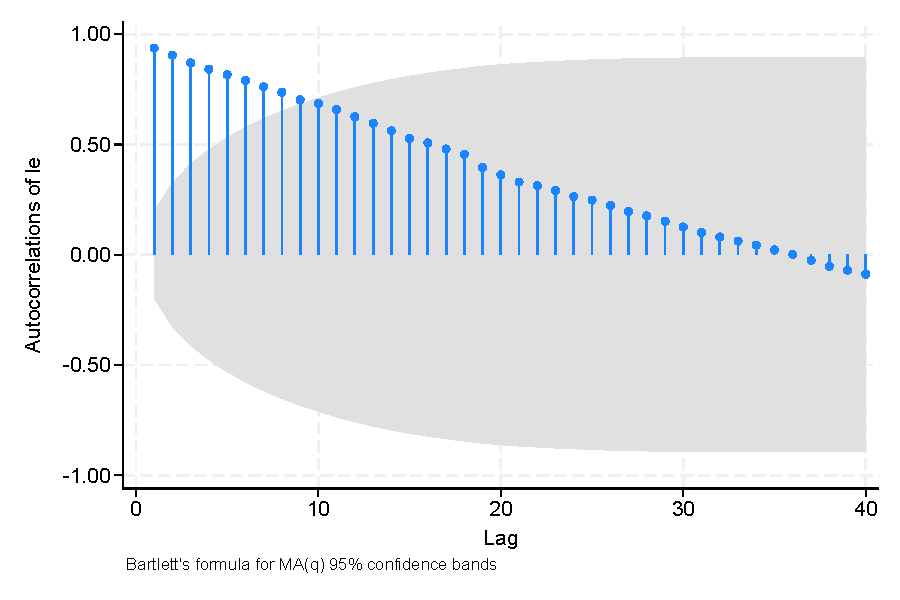
\includegraphics[width=0.45\textwidth]{image/acf.pdf} &
        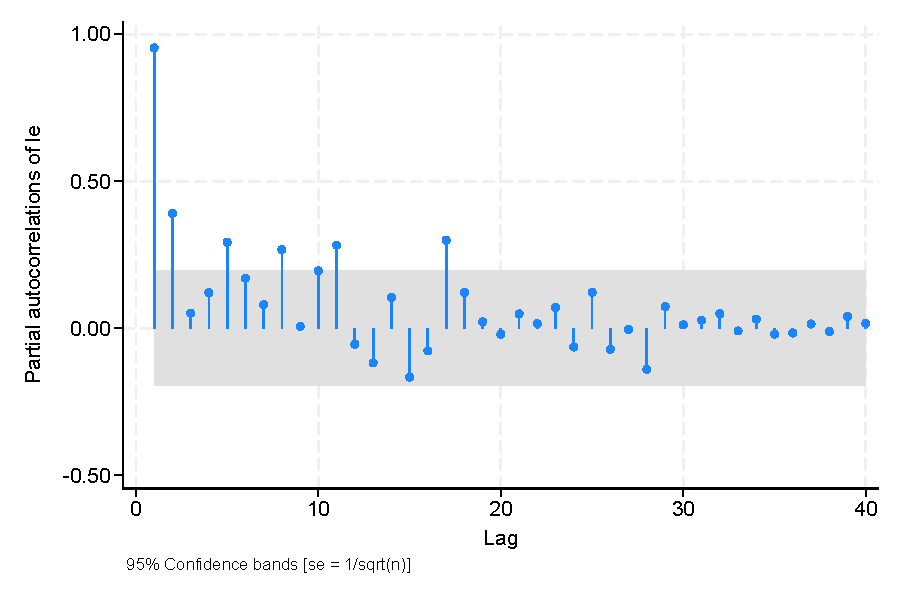
\includegraphics[width=0.45\textwidth]{image/pac.pdf}
    \end{tabular}}
    \caption{自相关图(左)和偏自相关图(右)}
    \label{fig:acf_pac}
\end{figure}

\begin{tcolorbox}[title=在 Stata 中应用多变量时间序列分析, colback=white, colframe=black, colbacktitle=white, coltitle=black,fonttitle=\bfseries]
\begin{lstlisting}[xleftmargin=2em, commentstyle=\color{black}]
webuse rates, clear
describe
summarize
tsset date, daily
twoway (line dow date, lcolor(blue)) (line nasdaq date, lcolor(red))
var dow nasdaq, lags(1/2)
vargranger
irf create var_rates, set(rates_irf) replace
irf graph irf, impulse(dow) response(nasdaq)
irf graph fevd
\end{lstlisting}
\vspace{-2em}
\begin{Verbatim}[commandchars=\\\{\},xleftmargin=2em]

111
\end{Verbatim}
\end{tcolorbox}

\subsection{空间计量经济学}
空间计量经济学处理的是截面或面板数据中,观测单元在地理空间上的相互依赖性。托布勒的地理学第一定律指出:“任何事物都与其他事物相关,但近处的事物比远处的事物更相关。”这种\textbf{空间依赖性(Spatial Dependence)}或\textbf{空间自相关(Spatial Autocorrelation)}违反了OLS观测独立的假定,会导致估计量有偏或无效。

\paragraph*{空间权重矩阵与空间自相关检验}
量化空间依赖性的关键工具是\textbf{空间权重矩阵(Spatial Weight Matrix, W)}。这是一个 $n \times n$ 的矩阵,其元素 $w_{ij}$ 反映了观测单元 $i$ 和 $j$ 之间的空间邻近程度。常见的设定包括:

\textbf{邻接矩阵}:如果 $i$ 和 $j$ 相邻,则 $w_{ij}=1$,否则为0。
\textbf{距离反比矩阵}:$w_{ij} = 1/d_{ij}$,其中 $d_{ij}$ 是两者间的距离。

通常对 $\mathbf{W}$ 进行行标准化,使得每行元素之和为1。

在进行空间回归之前,通常需要检验变量是否存在空间自相关。最常用的检验是\textbf{莫兰指数(Moran's I)},其值域通常在-1到1之间,正值表示空间集聚,负值表示空间分散,0表示空间随机分布。

\paragraph*{空间回归模型}
为处理空间依赖性,发展了多种空间回归模型:
\begin{enumerate}
    \item \textbf{空间滞后模型(Spatial Lag Model, SLM / SAR)}:假设因变量受到其邻近地区因变量的影响(空间溢出效应)。
    \begin{equation}
    \mathbf{Y} = \rho \mathbf{W}\mathbf{Y} + \mathbf{X}\boldsymbol{\beta} + \boldsymbol{\varepsilon}
    \end{equation}
    其中 $\rho$ 是空间自回归系数,衡量空间依赖的强度。

    \item \textbf{空间误差模型(Spatial Error Model, SEM)}:假设误差项存在空间相关性,即一个地区的冲击会影响到邻近地区。
    \begin{equation}
    \mathbf{Y} = \mathbf{X}\boldsymbol{\beta} + \mathbf{u}, \quad \text{其中 } \mathbf{u} = \lambda \mathbf{W}\mathbf{u} + \boldsymbol{\varepsilon}
    \end{equation}
    其中 $\lambda$ 是空间误差系数。

    \item \textbf{空间杜宾模型(Spatial Durbin Model, SDM)}:是更具一般性的模型,同时包含了因变量和自变量的空间滞后项。
    \begin{equation}
    \mathbf{Y} = \rho \mathbf{W}\mathbf{Y} + \mathbf{X}\boldsymbol{\beta} + \mathbf{W}\mathbf{X}\boldsymbol{\theta} + \boldsymbol{\varepsilon}
    \end{equation}
\end{enumerate}

在包含空间滞后项的模型(如SLM和SDM)中,系数 $\boldsymbol{\beta}$ 不能再解释为边际效应,因为存在反馈效应和溢出效应。需要分解为\textbf{直接效应(Direct Effect)}、\textbf{间接效应(Indirect Effect,即溢出效应)}和\textbf{总效应(Total Effect)}。

\begin{tcolorbox}[title=在 Stata 中估计空间滞后模型 (SLM/SAR), colback=white, colframe=black, colbacktitle=white, coltitle=black,fonttitle=\bfseries]
\begin{lstlisting}[xleftmargin=2em, commentstyle=\color{black}]
需要先安装 spxtregress, spmatrix 等命令
ssc install spxtregress, replace
ssc install spwmatrix, replace

使用Stata官方提供的意大利地区犯罪数据 (需要联网)
use "http://www.stata-press.com/data/r15/crime_e.dta", clear

创建空间权重矩阵 (基于各地区质心坐标)
spmatrix create contiguity W, xcoord(x) ycoord(y) normalize(row)

进行OLS回归,并检验残差的空间自相关性
reg pcrim po1 polpc conv
spatdiag, weights(W)

估计空间滞后模型 (SLM/SAR)
因变量 pcrim (人均犯罪率)
自变量 po1 (警察人数), polpc (人均警察), conv (定罪率)
spregress pcrim po1 polpc conv, dvarlag(W) mle
estat effects, dvarlag(W)
\end{lstlisting}
\vspace{-2em}
\begin{Verbatim}[commandchars=\\\{\},xleftmargin=2em]
. spatdiag, weights(W)
Moran's I test for spatial autocorrelation
Weights matrix: W
Number of obs = 93
Moran's I = 0.222
z-value = 3.655, p-value = 0.000
H0: No spatial autocorrelation. Test indicates rejection of H0.

. spregress pcrim po1 polpc conv, dvarlag(W) mle
(output omitted for brevity...)
Spatial autoregressive model                    Number of obs     =         93
Maximum likelihood estimation                   Wald chi2(3)      =      36.81
Prob > chi2       =     0.0000
Log likelihood = -262.58514                     Pseudo R2         =     0.3629

------------------------------------------------------------------------------
       pcrim | Coefficient  Std. err.      z    P>|z|     [95% conf. interval]
-------------+----------------------------------------------------------------
        po1 |   .1311756   .0298375     4.40   0.000     .0726955    .1896557
      polpc |  -33.80556   15.93815    -2.12   0.034    -65.04376   -2.567362
       conv |  -.0027157   .0004929    -5.51   0.000    -.0036817   -.0017497
       _cons |    1.73142   .2796195     6.19   0.000     1.183377    2.279463
-------------+----------------------------------------------------------------
W            |
       pcrim |   .3570373   .1197825     2.98   0.003     .1222683    .5918062
------------------------------------------------------------------------------
LR test of spatial lag rho=0: chi2(1) = 6.66, Prob > chi2 = 0.0099

. estat effects, dvarlag(W)
Direct, indirect, and total effects
Number of obs     =         93

------------------------------------------------------------------------------
             |            Direct   Indirect      Total
-------------+----------------------------------------------------------------
         po1 |         .1352632   .0805364   .2157996
      polpc |        -34.85871  -20.75487  -55.61358
        conv |        -.0028003  -.0016673  -.0044676
------------------------------------------------------------------------------
\end{Verbatim}
\end{tcolorbox}

莫兰指数检验结果显著,表明存在空间自相关,使用空间模型是必要的。spregress结果显示空间滞后项(W x pcrim)的系数 $\rho$ 显著为正,证实了犯罪率在地区间存在正向溢出。estat effects的分解结果显示,增加一个地区的警察人数,不仅会降低本地区的犯罪率(直接效应),还会通过溢出效应影响邻近地区的犯罪率(间接效应)。

\section{do算子与处置效应}

\subsection{虚拟变量}
\begin{enumerate}
	\item 虚拟变量的定义与生成方法
	\item 类别变量在回归中的处理
	\item 基准组选择与虚拟变量陷阱
	\item 交互项的引入与解释(特别是在异质效应分析中)
\end{enumerate}

\subsection{处置效应与偏误}
\begin{enumerate}
	\item 处置效应的定义(平均处理效应 ATE、ATT 等)
	\item 反事实框架(potential outcomes)
	\item 选择偏误问题及其来源(自选择、遗漏变量等)
	\item 识别策略的必要性与作用
\end{enumerate}

\section{两种策略}

\subsection{匹配法}
\begin{enumerate}
	\item 匹配法的基本思想与目的
	\item 匹配方法种类(最近邻匹配、半径匹配、核匹配等)
	\item 倾向得分(propensity score)的估计与匹配
	\item 匹配后平衡性检验
	\item 匹配法的优点与局限性
\end{enumerate}

\subsection{回归法}
\begin{enumerate}
	\item 回归模型在估计处置效应中的作用
	\item 包含控制变量的线性回归模型
	\item 交互项与异质性处置效应
	\item 回归调整与回归偏误
	\item 与匹配法的比较——异同
\end{enumerate}

\end{document}